% Options for packages loaded elsewhere
\PassOptionsToPackage{unicode}{hyperref}
\PassOptionsToPackage{hyphens}{url}
%
\documentclass[
]{article}
\usepackage{amsmath,amssymb}
\usepackage{iftex}
\ifPDFTeX
  \usepackage[T1]{fontenc}
  \usepackage[utf8]{inputenc}
  \usepackage{textcomp} % provide euro and other symbols
\else % if luatex or xetex
  \usepackage{unicode-math} % this also loads fontspec
  \defaultfontfeatures{Scale=MatchLowercase}
  \defaultfontfeatures[\rmfamily]{Ligatures=TeX,Scale=1}
\fi
% \usepackage{lmodern}
\ifPDFTeX\else
  % xetex/luatex font selection
\fi
% Use upquote if available, for straight quotes in verbatim environments
\IfFileExists{upquote.sty}{\usepackage{upquote}}{}
\IfFileExists{microtype.sty}{% use microtype if available
  \usepackage[]{microtype}
  \UseMicrotypeSet[protrusion]{basicmath} % disable protrusion for tt fonts
}{}
\makeatletter
\@ifundefined{KOMAClassName}{% if non-KOMA class
  \IfFileExists{parskip.sty}{%
    \usepackage{parskip}
  }{% else
    \setlength{\parindent}{0pt}
    \setlength{\parskip}{6pt plus 2pt minus 1pt}}
}{% if KOMA class
  \KOMAoptions{parskip=half}}
\makeatother
\usepackage{xcolor}
\usepackage{color}
\usepackage{fancyvrb}
\newcommand{\VerbBar}{|}
\newcommand{\VERB}{\Verb[commandchars=\\\{\}]}
\DefineVerbatimEnvironment{Highlighting}{Verbatim}{commandchars=\\\{\}}
% Add ',fontsize=\small' for more characters per line
\newenvironment{Shaded}{}{}
\newcommand{\AlertTok}[1]{\textcolor[rgb]{1.00,0.00,0.00}{\textbf{#1}}}
\newcommand{\AnnotationTok}[1]{\textcolor[rgb]{0.38,0.63,0.69}{\textbf{\textit{#1}}}}
\newcommand{\AttributeTok}[1]{\textcolor[rgb]{0.49,0.56,0.16}{#1}}
\newcommand{\BaseNTok}[1]{\textcolor[rgb]{0.25,0.63,0.44}{#1}}
\newcommand{\BuiltInTok}[1]{\textcolor[rgb]{0.00,0.50,0.00}{#1}}
\newcommand{\CharTok}[1]{\textcolor[rgb]{0.25,0.44,0.63}{#1}}
\newcommand{\CommentTok}[1]{\textcolor[rgb]{0.38,0.63,0.69}{\textit{#1}}}
\newcommand{\CommentVarTok}[1]{\textcolor[rgb]{0.38,0.63,0.69}{\textbf{\textit{#1}}}}
\newcommand{\ConstantTok}[1]{\textcolor[rgb]{0.53,0.00,0.00}{#1}}
\newcommand{\ControlFlowTok}[1]{\textcolor[rgb]{0.00,0.44,0.13}{\textbf{#1}}}
\newcommand{\DataTypeTok}[1]{\textcolor[rgb]{0.56,0.13,0.00}{#1}}
\newcommand{\DecValTok}[1]{\textcolor[rgb]{0.25,0.63,0.44}{#1}}
\newcommand{\DocumentationTok}[1]{\textcolor[rgb]{0.73,0.13,0.13}{\textit{#1}}}
\newcommand{\ErrorTok}[1]{\textcolor[rgb]{1.00,0.00,0.00}{\textbf{#1}}}
\newcommand{\ExtensionTok}[1]{#1}
\newcommand{\FloatTok}[1]{\textcolor[rgb]{0.25,0.63,0.44}{#1}}
\newcommand{\FunctionTok}[1]{\textcolor[rgb]{0.02,0.16,0.49}{#1}}
\newcommand{\ImportTok}[1]{\textcolor[rgb]{0.00,0.50,0.00}{\textbf{#1}}}
\newcommand{\InformationTok}[1]{\textcolor[rgb]{0.38,0.63,0.69}{\textbf{\textit{#1}}}}
\newcommand{\KeywordTok}[1]{\textcolor[rgb]{0.00,0.44,0.13}{\textbf{#1}}}
\newcommand{\NormalTok}[1]{#1}
\newcommand{\OperatorTok}[1]{\textcolor[rgb]{0.40,0.40,0.40}{#1}}
\newcommand{\OtherTok}[1]{\textcolor[rgb]{0.00,0.44,0.13}{#1}}
\newcommand{\PreprocessorTok}[1]{\textcolor[rgb]{0.74,0.48,0.00}{#1}}
\newcommand{\RegionMarkerTok}[1]{#1}
\newcommand{\SpecialCharTok}[1]{\textcolor[rgb]{0.25,0.44,0.63}{#1}}
\newcommand{\SpecialStringTok}[1]{\textcolor[rgb]{0.73,0.40,0.53}{#1}}
\newcommand{\StringTok}[1]{\textcolor[rgb]{0.25,0.44,0.63}{#1}}
\newcommand{\VariableTok}[1]{\textcolor[rgb]{0.10,0.09,0.49}{#1}}
\newcommand{\VerbatimStringTok}[1]{\textcolor[rgb]{0.25,0.44,0.63}{#1}}
\newcommand{\WarningTok}[1]{\textcolor[rgb]{0.38,0.63,0.69}{\textbf{\textit{#1}}}}
\usepackage{longtable,booktabs,array}
\usepackage{calc} % for calculating minipage widths
% Correct order of tables after \paragraph or \subparagraph
\usepackage{etoolbox}
\makeatletter
\patchcmd\longtable{\par}{\if@noskipsec\mbox{}\fi\par}{}{}
\makeatother
% Allow footnotes in longtable head/foot
\IfFileExists{footnotehyper.sty}{\usepackage{footnotehyper}}{\usepackage{footnote}}
\makesavenoteenv{longtable}
\usepackage{graphicx}
\makeatletter
\def\maxwidth{\ifdim\Gin@nat@width>\linewidth\linewidth\else\Gin@nat@width\fi}
\def\maxheight{\ifdim\Gin@nat@height>\textheight\textheight\else\Gin@nat@height\fi}
\makeatother
% Scale images if necessary, so that they will not overflow the page
% margins by default, and it is still possible to overwrite the defaults
% using explicit options in \includegraphics[width, height, ...]{}
\setkeys{Gin}{width=\maxwidth,height=\maxheight,keepaspectratio}
% Set default figure placement to htbp
\makeatletter
\def\fps@figure{htbp}
\makeatother
\setlength{\emergencystretch}{3em} % prevent overfull lines
\providecommand{\tightlist}{%
  \setlength{\itemsep}{0pt}\setlength{\parskip}{0pt}}
\setcounter{secnumdepth}{5}
\ifLuaTeX
\usepackage[bidi=basic]{babel}
\else
\usepackage[bidi=default]{babel}
\fi
\babelprovide[main,import]{english}
% get rid of language-specific shorthands (see #6817):
\let\LanguageShortHands\languageshorthands
\def\languageshorthands#1{}
\makeatletter
\@ifpackageloaded{subcaption}{}{\usepackage{subcaption}}
\@ifpackageloaded{caption}{}{\usepackage{caption}}
\captionsetup[subfigure]{margin=0.5em}
\AtBeginDocument{%
\renewcommand*\figurename{Figure}
\renewcommand*\tablename{Table}
}
\AtBeginDocument{%
\renewcommand*\listfigurename{List of Figures}
\renewcommand*\listtablename{List of Tables}
}
\newcounter{pandoccrossref@subfigures@footnote@counter}
\newenvironment{pandoccrossrefsubfigures}{%
\setcounter{pandoccrossref@subfigures@footnote@counter}{0}
\begin{figure}\centering%
\gdef\global@pandoccrossref@subfigures@footnotes{}%
\DeclareRobustCommand{\footnote}[1]{\footnotemark%
\stepcounter{pandoccrossref@subfigures@footnote@counter}%
\ifx\global@pandoccrossref@subfigures@footnotes\empty%
\gdef\global@pandoccrossref@subfigures@footnotes{{##1}}%
\else%
\g@addto@macro\global@pandoccrossref@subfigures@footnotes{, {##1}}%
\fi}}%
{\end{figure}%
\addtocounter{footnote}{-\value{pandoccrossref@subfigures@footnote@counter}}
\@for\f:=\global@pandoccrossref@subfigures@footnotes\do{\stepcounter{footnote}\footnotetext{\f}}%
\gdef\global@pandoccrossref@subfigures@footnotes{}}
\@ifpackageloaded{float}{}{\usepackage{float}}
\floatstyle{ruled}
\@ifundefined{c@chapter}{\newfloat{codelisting}{h}{lop}}{\newfloat{codelisting}{h}{lop}[chapter]}
\floatname{codelisting}{Listing}
\newcommand*\listoflistings{\listof{codelisting}{List of Listings}}
\makeatother
\ifLuaTeX
  \usepackage{selnolig}  % disable illegal ligatures
\fi
\usepackage[]{natbib}
\bibliographystyle{plainnat}
\usepackage{bookmark}
\IfFileExists{xurl.sty}{\usepackage{xurl}}{} % add URL line breaks if available
\urlstyle{same}
\hypersetup{
  pdftitle={A Reproducible Multi-Phase Literature-Review Pipeline for Exoplanet Atmospheres},
  pdfauthor={Daniel Ari Friedman},
  pdflang={en},
  colorlinks=true,linkcolor=red,urlcolor=red,citecolor=red,anchorcolor=red,filecolor=red,
  pdfcreator={LaTeX via pandoc}}

\title{A Reproducible Multi-Phase Literature-Review Pipeline for
Exoplanet Atmospheres}
\author{Daniel Ari Friedman}
\date{}

\IfFileExists{seqsplit.sty}{\usepackage{seqsplit}}{\newcommand{\seqsplit}[1]{#1}}
\protected\def\breakseq#1{\seqsplit{#1}}
\protected\def\breaktt#1{\begingroup\ttfamily\seqsplit{#1}\endgroup}
\title{A Reproducible Multi-Phase Literature-Review Pipeline for Exoplanet Atmospheres}
\author{Daniel Ari Friedman\\\footnotesize{Active Inference Institute}\\\footnotesize{\texttt{daniel@activeinference.institute}}\\\footnotesize{\href{https://orcid.org/0000-0001-6232-9096}{ORCID: 0000-0001-6232-9096}} \\ \footnotesize{DOI: forthcoming}}
\date{\today}

% Core mathematics
\usepackage{amsmath}
\usepackage{amssymb}
\usepackage{amsfonts}
\usepackage{amsthm}

% Document layout
\usepackage[margin=1.8cm]{geometry}
\usepackage{float}
\usepackage{graphicx}
\usepackage[section]{placeins}  % Constrain floats to their section
\renewcommand{\floatpagefraction}{0.7}  % Require 70% fill for float-only pages
\renewcommand{\topfraction}{0.9}        % Allow large top floats

% Tables
\usepackage{booktabs}
\usepackage{longtable}
\usepackage{array}
\usepackage{multirow}

% Code listings
\usepackage{listings}

% Typography and formatting
\usepackage{microtype}
\usepackage{xcolor}

% Cross-references and citations (hyperref loaded by other packages with [unicode]; set options only)
\hypersetup{colorlinks=true,linkcolor=red,citecolor=red,urlcolor=red}
\usepackage[capitalise,noabbrev]{cleveref}
% NOTE: natbib is auto-injected by Pandoc via --natbib (which also writes
% \bibliographystyle{plainnat}). Do not re-declare \usepackage{natbib} here
% or LaTeX will error with "Option clash for package natbib".

% Figure caption formatting
\usepackage{caption}

% Algorithm typesetting
\IfFileExists{algorithm2e.sty}{\usepackage[ruled,vlined]{algorithm2e}}{}

% The manuscript uses these environments in the technical appendix.  Define the
% parent counter before the subordinate environments so XeLaTeX has no hidden
% preamble dependency.
\newtheorem{theorem}{Theorem}[section]
\newtheorem{remark}[theorem]{Remark}
\newtheorem{example}[theorem]{Example}

% Custom commands for domain notation
\newcommand{\FEP}{\textsc{fep}}
\newcommand{\AIF}{\textsc{aif}}
\newcommand{\KL}{\mathrm{KL}}
\newcommand{\E}{\mathbb{E}}
\newcommand{\F}{\mathcal{F}}

% NMF and topic modeling notation
\newcommand{\matW}{\mathbf{W}}  % NMF document-topic matrix
\newcommand{\matH}{\mathbf{H}}  % NMF topic-term matrix
\newcommand{\matV}{\mathbf{V}}  % NMF document-term matrix
\newcommand{\tfidf}{\text{TF-IDF}}
\newcommand{\cagr}{\text{CAGR}}
\newcommand{\score}{\operatorname{score}}
\newcommand{\corpusvar}[1]{\texttt{\{\{#1\}\}}}
\newcommand{\scoreH}[1]{\text{score}(H_{#1})}
\newcommand{\EBM}{\textsc{ebm}}
\newcommand{\VFE}{\mathcal{F}_{\text{VFE}}}
\newcommand{\RBM}{\textsc{rbm}}

% Assertion and evidence notation
\newcommand{\supports}{\mathrel{\text{supports}}}
\newcommand{\contradicts}{\mathrel{\text{contradicts}}}
\newcommand{\neutral}{\mathrel{\text{neutral}}}

% Domain taxonomy shorthands
\newcommand{\domA}{\text{A}}
\newcommand{\domB}{\text{B}}
\newcommand{\domC}{\text{C}}

% Evidence-score and growth metrics
\newcommand{\EFE}{\mathbf{G}}       % Evidence-score matrix
\newcommand{\doubling}{t_d}         % Doubling time
\newcommand{\meangrowth}{\bar{g}}   % Mean year-over-year growth rate

% Corpus and scoring notation
\newcommand{\Nstart}{N_{\text{start}}}  % Publication count in first year
\newcommand{\Nend}{N_{\text{end}}}      % Publication count in last year
\newcommand{\SH}{S(H)}                  % Supporting assertions for H
\newcommand{\CH}{C(H)}                  % Contradicting assertions for H
\newcommand{\AH}{A(H)}                  % All assertions for H

% Tool and project shorthands
\newcommand{\nanopub}{\textsc{np}}      % Nanopublication shorthand
\newcommand{\ollama}{\textsc{Ollama}}   % Ollama LLM server
\newcommand{\pymdp}{\textsc{pymdp}}     % pymdp library

% Network and graph operators
\DeclareMathOperator{\PageRank}{PageRank}  % PageRank operator

\begin{document}
\begin{titlepage}
\centering
\vspace*{2cm}
{\LARGE\bfseries A Reproducible Multi-Phase Literature-Review Pipeline for Exoplanet Atmospheres\par}
\vspace{0.75em}
{\large Synthetic Fixture Exemplar with Source-Aware Retrieval and Optional LLM Analysis\par}
\vfill
\makeatletter
{\@author\par}
\vspace{1em}
{\@date\par}
\makeatother
\vfill
\end{titlepage}
\thispagestyle{empty}
\tableofcontents
\newpage

\section{Abstract}\label{abstract}

We specify a reproducible advanced literature-review workflow for
rapidly changing domains in which a single query does not adequately
represent methodological or temporal variation. The exemplar is
configured for exoplanet atmospheric composition and separates
foundation, James Webb Space Telescope, and molecular-detection phases.

The design is informed by systematic-review reporting practice
\citep{page2021prisma}, but this repository release is a methods
exemplar rather than a completed systematic review: its default corpus
is synthetic and its phase boundaries, search coverage, and domain
interpretation require review for any live application.

The pipeline combines multi-engine retrieval, canonical de-duplication,
deterministic screening, optional LLM-assisted classification, full-text
assessment, bibliometrics, knowledge-graph construction, visualization,
reproducibility assessment, and export. Each stage has a declared input,
output, method reference, and definition of done in
\breaktt{methods\_pipeline.yaml}. The numbered scripts are thin adapters;
reusable computation is tested in \texttt{src/}.

The manuscript is generated from configuration and recorded artifacts.
Offline runs use a clearly labelled synthetic fixture corpus with
reserved identifiers and generated authors; they exercise pipeline
behavior and are not evidence about \{\{SEARCH\_TERM\}\}. Live runs must
retain retrieval reports, source provenance, claim classifications, and
the exact configuration needed to interpret reported results.

The contribution is therefore infrastructural: it makes phase-aware
search design, evidence boundaries, accessibility metadata, and
reproducibility checks explicit while leaving domain claims subject to
source-backed review.

\textbf{Keywords:} \{\{KEYWORDS\_LIST\}\}

\newpage

\section{Introduction}\label{introduction}

Rapidly changing fields require literature reviews that preserve the
distinction between what was searched, what was retrieved, what was
assessed, and what can be claimed. A single broad query hides
phase-specific coverage and makes it difficult to explain how records
entered a synthesis. This project treats a literature review as a
reproducible data pipeline: configuration defines the review design,
source adapters acquire records, analysis modules produce evidence
artifacts, and rendering turns those artifacts into an auditable
manuscript.

The reporting surface follows the spirit of systematic-review
transparency \citep{page2021prisma} without implying that the bundled
fixture satisfies a domain protocol. A live review must define
eligibility criteria, search dates, source coverage, screening
procedures, and a domain-appropriate synthesis plan before its results
are interpreted.

The bundled configuration targets \textbf{\{\{SEARCH\_TERM\_TITLE\}\}}.
It defines three ordered phases for foundational methods, JWST-era
observations, and molecular detection. The phase labels are
configuration, not conclusions: a live review must justify its
boundaries and update its claim ledger when the domain or search
strategy changes.

\subsection{Research Questions}\label{research-questions}

\begin{enumerate}
\def\labelenumi{\arabic{enumi}.}
\tightlist
\item
  \textbf{Coverage and retrieval.} Which engines, queries, filters, and
  identifiers contributed records to each phase, and where are the known
  coverage limits?
\item
  \textbf{Structure.} How do subfields, topics, authors, venues, and
  citation links vary across the configured phases?
\item
  \textbf{Evidence.} Which claims are supported by source-backed
  records, which remain pending, and which are only properties of the
  synthetic fixture?
\item
  \textbf{Reproducibility.} Can a clean run regenerate the data,
  figures, reports, and manuscript without unexplained differences?
\end{enumerate}

\subsection{Scope and contribution}\label{scope-and-contribution}

The project contributes a reusable workflow rather than a domain
conclusion. Retrieval and de-duplication preserve source observations;
full-text assessment records access status; bibliometrics and graph
construction expose descriptive structure; and the claim ledger
separates fixture, configured, and source-backed statements. Subjective
editorial, scientific, and visual judgments remain explicit review items
even when all deterministic gates pass.

Every generated number in the rendered manuscript must come from an
artifact listed in the manifest and be traceable to the relevant method
stage. Missing, stale, or misclassified evidence is a release finding,
not a value to be filled by hand.

\newpage

\section{Methods Overview}\label{methods-overview}

The project is an eleven-stage, file-system-backed pipeline.
\breaktt{methods\_pipeline.yaml} is the executable contract: each stage
names its method, dependencies, inputs, outputs, definition of done, and
stable failure code. Business logic lives in tested \texttt{src/}
modules; numbered scripts only perform bootstrapping, argument parsing,
orchestration, and boundary I/O.

\subsection{Pipeline stages}\label{pipeline-stages}

\begin{enumerate}
\def\labelenumi{\arabic{enumi}.}
\tightlist
\item
  \textbf{Multi-phase retrieval} (\breaktt{01\_multi\_phase\_search.py})
  acquires records or runs the labelled offline fixture, applies
  configured filters, de-duplicates identifiers, and writes phase
  corpora plus \breaktt{phase\_metadata.json} and the
  \breaktt{phase\_artifact\_manifest.json} phase-to-artifact provenance
  map.
\item
  \textbf{Corpus analysis} (\breaktt{02\_meta\_analysis\_pipeline.py})
  computes subfields, temporal trends, TF-IDF/topics, and
  citation-network artifacts.
\item
  \textbf{Knowledge graph construction}
  (\breaktt{03\_build\_knowledge\_graph.py}) optionally extracts
  assertions and phase-aware hypothesis evidence; disabled or unmeasured
  LLM outputs remain explicitly pending.
\item
  \textbf{Visualization} (\breaktt{04\_generate\_figures.py}) renders
  figures from analysis artifacts and records source paths, hashes,
  captions, and alt text in the figure registry.
\item
  \textbf{Manuscript hydration} (\breaktt{05\_inject\_variables.py})
  computes variables from outputs and writes rendered Markdown without
  changing source sections.
\item
  \textbf{Full-text assessment} (\breaktt{06\_fulltext\_assessment.py})
  records abstract, open-access, and PDF availability; downloading is
  opt-in and network-gated.
\item
  \textbf{Literature evaluation}
  (\breaktt{07\_literature\_evaluation.py}) applies configured quality
  and fixture-honesty checks.
\item
  \textbf{Research dispatch} (\breaktt{08\_deep\_research\_dispatch.py})
  replays a recorded report by default and exposes live provider
  dispatch only as an explicit opt-in.
\item
  \textbf{Bibliography export} (\breaktt{09\_export\_bibliography.py})
  writes a deterministic bibliography from the retained corpus and
  source references.
\item
  \textbf{Reproducibility assessment}
  (\breaktt{10\_reproducibility\_assessment.py}) records workflow and
  source-consumption evidence.
\item
  \textbf{Publication validation} (\breaktt{11\_validate\_outputs.py})
  validates artifact, evidence, figure, and report contracts before the
  shared publication audit runs.
\end{enumerate}

\subsection{Reproducibility model}\label{reproducibility-model}

The offline path uses a deterministic synthetic fixture with reserved
identifiers and generated authors. It is useful for CI and structural
testing only; it is never a substitute for a representative live review.
A live run must preserve the retrieval report, engine status, source
identifiers, configuration, and claim classifications. Seeds and
timestamp-free serializers are used where the pipeline supports exact
replay.

\subsection{Configuration surface}\label{configuration-surface}

\breaktt{manuscript/config.yaml} owns search terms, engines, phase
boundaries, filters, sampling seeds, full-text policy, embedding
settings, knowledge-graph settings, hypotheses, and subfield taxonomy.
\breaktt{domain\_profile.yaml} owns package and gate expectations;
\breaktt{experiment\_plan.yaml} records the review design;
\breaktt{data/claim\_ledger.yaml} records the provenance tier and
fixture/synthetic status of manuscript-facing claims.

\newpage

\section{Retrieval and
De-duplication}\label{retrieval-and-de-duplication}

Retrieval dispatches the configured query across \{\{N\_ENGINES\}\}
independent literature engines (\{\{ENGINE\_LIST\}\}). Each engine is an
isolated adapter exposing a uniform
\texttt{search(query)\ -\textgreater{}\ list{[}Record{]}} interface;
engines that are keyless --- arXiv, OpenAlex \citep{priem2022openalex},
Crossref \citep{hendricks2020crossref}, PubMed/Entrez
\citep{sayers2022entrez}, SovietRxiv / RussiaRxiv, ChinaRxiv, Europe
PMC, and bioRxiv/medRxiv --- need no credentials, while Semantic Scholar
\citep{kinney2023semantic} uses a key when present. SovietRxiv is a
translated archive of Soviet-era scientific preprints sourced from
Math-Net.Ru and CyberLeninka \citep{sovietrxiv}; ChinaRxiv serves
translated Chinese preprints from ChinaXiv via the same unified API.
Both retain original-language PDFs alongside each translation, and their
polite rate-limit pool (300/min vs 30/min anonymous) is activated by an
optional \texttt{X-API-Email} header. Europe PMC is a keyless biomedical
aggregator covering PubMed, PMC, patents, and preprints in a single
search call. bioRxiv/medRxiv share one unified date-window + cursor API;
unlike the other engines it is not a free-text search endpoint, so the
adapter walks the date window page by page and keeps only records whose
title and abstract match every query term client-side. Optional
full-text resolution queries Unpaywall \citep{piwowar2018state} for
open-access locations. \textbf{Multiple dispatch degrades gracefully}:
an engine that is disabled in the configuration, lacks a required key,
or cannot reach the network returns a \emph{skipped} status, and the run
completes from the remaining engines plus the committed offline corpus.

\subsection{Engine Details}\label{engine-details}

Each engine adapter follows a uniform contract: a module-level API URL
constant, a pure \texttt{\_parse\_*} parser function, and a
\texttt{search\_*} entry point with pagination, retry, and graceful
error handling. All functions accept an injectable \texttt{base\_url}
parameter for hermetic testing with \breaktt{pytest-httpserver} --- no
engine hardcodes its URL inside the function body.

\begin{longtable}[]{@{}
  >{\raggedright\arraybackslash}p{(\columnwidth - 6\tabcolsep) * \real{0.2500}}
  >{\raggedright\arraybackslash}p{(\columnwidth - 6\tabcolsep) * \real{0.2500}}
  >{\raggedright\arraybackslash}p{(\columnwidth - 6\tabcolsep) * \real{0.2500}}
  >{\raggedright\arraybackslash}p{(\columnwidth - 6\tabcolsep) * \real{0.2500}}@{}}
\toprule\noalign{}
\begin{minipage}[b]{\linewidth}\raggedright
Engine
\end{minipage} & \begin{minipage}[b]{\linewidth}\raggedright
Rate limit
\end{minipage} & \begin{minipage}[b]{\linewidth}\raggedright
Pagination
\end{minipage} & \begin{minipage}[b]{\linewidth}\raggedright
Auth
\end{minipage} \\
\midrule\noalign{}
\endhead
\bottomrule\noalign{}
\endlastfoot
arXiv & 3s between requests & 100/page, offset & Keyless \\
Semantic Scholar & 1 req/s (unauth.) & 100/page, offset & Optional
key \\
OpenAlex & Polite pool (mailto) & 200/page, cursor & Keyless \\
Crossref & Polite pool (mailto) & 1,000/page, offset & Keyless \\
PubMed & NCBI usage policy & retstart/retmax & Keyless \\
SovietRxiv & 30/min (300/min polite) & 1--100/page, cursor &
\texttt{X-API-Email} \\
ChinaRxiv & 30/min (300/min polite) & 1--100/page, cursor &
\texttt{X-API-Email} \\
Europe PMC & about 10 req/s (undocumented hard limit) & Up to
1,000/page & Keyless \\
bioRxiv/medRxiv & No documented limit & 100/page fixed, cursor &
Keyless \\
\end{longtable}

Every new search writes \breaktt{output/data/retrieval\_report.json}, a
timestamp-free report that records each attempted, skipped, or failed
source with fetched, new-record, and duplicate counts. A zero-result
response is therefore distinguishable from a disabled adapter or an HTTP
failure. The committed corpus predates that report contract, so this
paper intentionally does not reconstruct source-specific counts from the
merged corpus.

\subsection{Canonical Identifier
Hierarchy}\label{canonical-identifier-hierarchy}

Heterogeneous records are reconciled by a \textbf{canonical identifier
hierarchy} --- DOI \(>\) arXiv ID \(>\) Semantic Scholar ID \(>\)
OpenAlex ID \(>\) a stable digest of the normalized title. When two
records share a canonical identifier they are merged, keeping the
version with the most complete metadata (a count of non-None optional
fields). The DOI is normalized: case-folded, resolver-prefix stripped,
so the same paper returned by two engines under case/format-variant DOIs
merges. For this run, \{\{DOI\_COUNT\}\} records carry DOIs,
\{\{OPENALEX\_ID\_COUNT\}\} carry OpenAlex IDs, and
\{\{ARXIV\_ID\_COUNT\}\} carry arXiv IDs. The de-duplicated corpus for
this run holds \(N = {{CORPUS_SIZE}}\) records published across
\{\{YEAR\_START\}\}--\{\{YEAR\_END\}\}.

\subsection{Relevance Filtering}\label{relevance-filtering}

After de-duplication, a relevance filter drops papers whose title and
abstract contain none of the configured relevance keywords
(\{\{KEYWORDS\_RELEVANCE\}\}). Keywords are matched case-insensitively;
an empty keyword list is treated as no filter to avoid silently wiping
the corpus. A year filter then excludes papers published before the
configured start year (\{\{YEAR\_START\}\}).

\newpage

\section{Full Text, Language, and
Embeddings}\label{full-text-language-and-embeddings}

Beyond bibliographic metadata, the pipeline mines the textual content of
each record. This stage bridges the gap between a bibliographic
inventory and a semantic understanding of the literature.

\subsection{Full-Text Availability}\label{full-text-availability}

An open-access resolver maps each record to a downloadable PDF where one
exists (a known \texttt{pdf\_url}, or an Unpaywall lookup by DOI), and
an opt-in, network-gated downloader fetches it to a deterministic path.
Full-text availability is summarized without requiring any download, so
the offline default still reports coverage. For this run:

\begin{itemize}
\tightlist
\item
  \textbf{Abstract coverage}: \{\{ABSTRACT\_COVERAGE\_PCT\}\}\% of
  records (\{\{ABSTRACT\_COUNT\}\} of \{\{CORPUS\_SIZE\}\}) carry an
  abstract; \{\{NO\_ABSTRACT\_COUNT\}\} records lack one.
\item
  \textbf{Open-access status}: \{\{OA\_PCT\}\}\% of records are open
  access (\{\{OA\_COUNT\}\} records); the remainder are closed or
  unknown.
\item
  \textbf{PDF availability}: \{\{PDF\_AVAIL\_PCT\}\}\% of records
  (\{\{PDF\_AVAIL\_COUNT\}\}) have a direct PDF link;
  \{\{PUBLISHER\_PDF\_COUNT\}\} have a publisher PDF, and
  \{\{NO\_FULLTEXT\_COUNT\}\} have no full-text source available.
\end{itemize}

The identifier coverage for this corpus is: \{\{DOI\_COUNT\}\} DOIs,
\{\{OPENALEX\_ID\_COUNT\}\} OpenAlex IDs, and \{\{ARXIV\_ID\_COUNT\}\}
arXiv IDs. DOI coverage dominates and supports cross-engine
de-duplication.

\subsection{Language and Entity
Extraction}\label{language-and-entity-extraction}

Titles, abstracts, and (when present) full text are tokenized and
reduced to keyphrases and named entities by offline, dependency-light
extractors --- no mandatory LLM. Term-frequency statistics drive a
TF-IDF representation over a \{\{NUM\_VOCAB\_FEATURES\}\}-feature
vocabulary. The most frequent terms in the corpus are:
\{\{TOP\_VOCAB\_TERMS\}\}. These terms reflect the configured domain and
the records retained by the retrieval and filtering policy;
fixture-derived terms are not evidence about the live field.

\subsection{Embeddings}\label{embeddings}

Every title, abstract, and full text is embedded into a shared vector
space by a deterministic, offline method --- TF-IDF followed by
truncated SVD, i.e.~latent semantic analysis
\citep{deerwester1990indexing}. The embedding dimensionality is 50
components (configurable via
\breaktt{project\_config.embeddings.n\_components}), and the TF-IDF
vocabulary is capped at \{\{NUM\_VOCAB\_FEATURES\}\} features
(configurable via \breaktt{project\_config.embeddings.max\_features}).
The embedding is byte-stable across runs: the same input text always
yields identical vectors, so the derived similarity matrix,
nearest-neighbour lists, clusters, and two-dimensional projection are
all reproducible.

An optional transformer backend can be enabled by setting
\breaktt{project\_config.embeddings.method:\ transformer} (requires the
\texttt{embeddings} extra), which upgrades the embedding fidelity
without changing the interface or downstream analysis.

The embeddings support semantic retrieval over the corpus and feed two
visualizations: a PCA two-dimensional projection ((Figure pca
embeddings)) that maps the topical geography of the literature, and a
hierarchical clustering dendrogram ((Figure dendrogram)) that reveals
the similarity structure of the document collection.

\newpage

\section{Bibliometric and Temporal
Analysis}\label{bibliometric-and-temporal-analysis}

Descriptive statistics summarize the corpus along every available axis:
counts by year, venue, and author; citation-count distributions; and
author productivity. Temporal analysis fits the publication time series,
reporting a compound annual growth rate of \{\{CAGR\_PCT\}\}\% across
\{\{YEAR\_START\}\}--\{\{YEAR\_END\}\} (a span of \{\{YEAR\_SPAN\}\}
years), with a mean year-over-year growth rate of
\{\{MEAN\_YOY\_GROWTH\_PCT\}\}\% and a doubling time of
\{\{DOUBLING\_TIME\}\} years. The peak publication year is
\{\{PEAK\_YEAR\}\} with \{\{PEAK\_YEAR\_PUBS\}\} records.

\subsection{Growth Metrics}\label{growth-metrics}

The compound annual growth rate (CAGR) is computed as:

\[
\text{CAGR} = \left(\frac{N_{\text{end}}}{N_{\text{start}}}\right)^{1/(\text{year span})} - 1
\]

where \(N_{\text{start}}\) is the publication count in the first year
(\{\{YEAR\_START\}\}) and \(N_{\text{end}}\) is the count in the last
year (\{\{YEAR\_END\}\}). The mean year-over-year growth rate
\(\bar{g}\) is the arithmetic mean of annual ratios. The doubling time
is \(t_d = \ln(2) / \ln(1 + \text{CAGR})\). These metrics are stored in
\breaktt{temporal\_analysis.json} and injected into the manuscript at
render time.

\subsection{Subfield Classification}\label{subfield-classification}

Subfield classification assigns each record to one of
\{\{N\_SUBFIELDS\}\} configurable buckets (\{\{SUBFIELD\_LIST\}\}) by
priority-aware keyword matching; the taxonomy is defined entirely in
configuration (\breaktt{project\_config.subfield\_keywords}). The largest
bucket is \textbf{\{\{TOP\_SUBFIELD\}\}} at \{\{TOP\_SUBFIELD\_PCT\}\}\%
of the classified corpus. A per-subfield temporal breakdown
(\breaktt{subfield\_timeline.json}) tracks how each sub-area has grown
over time, enabling identification of emerging or declining research
threads.

\subsection{Topic Modeling}\label{topic-modeling}

A TF-IDF term-weighting of titles and abstracts \citep{salton1988term}
feeds non-negative matrix factorization (NMF) \citep{lee1999learning},
implemented with scikit-learn \citep{pedregosa2011scikit}. NMF
decomposes the document-term matrix
\(\mathbf{V} \approx \mathbf{W} \mathbf{H}\), where \(\mathbf{W}\) is
the document-topic matrix and \(\mathbf{H}\) is the topic-term matrix.
The factorization extracts \{\{NUM\_TOPICS\}\} latent topics that
cross-cut the keyword taxonomy. The random seed is fixed at 42 for
reproducibility. The reporting follows established systematic-review
practice \citep{page2021prisma}, with every figure and statistic
traceable to a committed artifact.

\newpage

\section{Optional Knowledge-Graph
Layer}\label{optional-knowledge-graph-layer}

An optional, \textbf{LLM-gated} stage lifts the corpus from
bibliometrics to hypothesis-level evidence. For each eligible record, a
local language model (Ollama, default model \texttt{gemma3:4b}) extracts
structured \emph{assertions}. Each assertion encodes a direction
(supports, contradicts, or neutral), a confidence score, and a short
natural-language justification against one of the \{\{N\_HYPOTHESES\}\}
hypotheses declared in configuration. Assertions are serialized as
RDF-compatible nanopublications \citep{kuhn2016decentralized} and scored
by a citation-weighted evidence function.

\subsection{Assertion Model}\label{assertion-model}

Each assertion \(a\) encodes:

\begin{itemize}
\tightlist
\item
  \textbf{Direction}: \(\text{supports}\), \(\text{contradicts}\), or
  \(\text{neutral}\) with respect to a hypothesis \(H\)
\item
  \textbf{Confidence}: a score \(c_a \in [0, 1]\) from the LLM
\item
  \textbf{Citation weight}: \(\log(1 + n_{\text{cites}})\), where
  \(n_{\text{cites}}\) is the citation count of the asserting paper
\end{itemize}

The evidence score for hypothesis \(H\) is:

\[
\text{score}(H) = \frac{\sum_{a \in A(H)^+} c_a \cdot \log(1 + n_{\text{cites}}(a)) -
\sum_{a \in A(H)^-} c_a \cdot \log(1 + n_{\text{cites}}(a))}
{\sum_{a \in A(H)} c_a \cdot \log(1 + n_{\text{cites}}(a))}
\]

where \(A(H)^+\) is the set of supporting assertions and \(A(H)^-\) the
contradicting ones. The score ranges from \(-1\) (all evidence
contradicts) to \(+1\) (all evidence supports).

\subsection{Incremental Extraction}\label{incremental-extraction}

Assertion extraction is \textbf{incremental and resumable}: assertions
are appended to \breaktt{nanopublications.jsonl} at configurable
checkpoint intervals (default: 50 papers). On restart, already-processed
papers are skipped automatically, so a long extraction run that is
interrupted can resume without re-processing. The
\breaktt{-\/-clear-assertions} flag discards previous results for a fresh
start.

\subsection{Gating and Defaults}\label{gating-and-defaults}

This stage is optional and gated by language-model availability. With no
language model configured, the hypothesis evidence scores read
\emph{pending}. When Ollama is explicitly configured and the extraction
stage completes, scores are populated from the recorded,
citation-weighted assertions. The hypotheses themselves, including their
names and scope, come from configuration and are reported regardless of
whether scoring has run.

The hypotheses explored in this instance are: \{\{HYPOTHESIS\_LIST\}\}.

\newpage

\section{Visualization and Manuscript
Injection}\label{visualization-and-manuscript-injection}

\subsection{Figure Generation}\label{figure-generation}

Figures are rendered headlessly (matplotlib Agg backend) and
deterministically from the analysis artifacts: subfield distributions,
the publication growth curve, the citation network, topic-term bars, a
term cloud, and embedding projections. All figures use a
colourblind-safe palette (Wong 2011, 8 colours) with high-contrast
labels at \(\geq 16\)pt. This run produced \{\{NUM\_FIGURES\}\} figures
at 300 DPI. The full figure set includes:

\begin{itemize}
\tightlist
\item
  \textbf{Field overview}: field summary and subfield distribution
  ((Figure field summary; Figure subfield distribution))
\item
  \textbf{Temporal}: growth curve and subfield timeline ((Figure growth
  curve; Figure subfield timeline))
\item
  \textbf{Citation network}: network layout and degree distribution
  ((Figure citation network; Figure degree distribution))
\item
  \textbf{Hypothesis}: dashboard and evidence timeline ((Figure
  hypothesis dashboard))
\item
  \textbf{Text analytics}: word cloud, topic-term bars, PCA embeddings,
  term heatmap, dendrogram, and co-occurrence matrix ((Figure word
  cloud; Figure topic term bars; Figure pca embeddings; Figure term
  heatmap; Figure dendrogram; Figure cooccurrence matrix))
\end{itemize}

Each figure is registered in \breaktt{figure\_registry.json} with its
source data file, generation parameters, and SHA-256 hash, binding the
visual output to the exact pipeline run.

\subsection{Variable Injection}\label{variable-injection}

The manuscript itself is generated, not hand-maintained. A variable
computation step reads the configuration and the pipeline outputs and
emits a flat table of named values; an injection step substitutes each
named placeholder in these Markdown sections with its computed value
before rendering. Because the substitution is total, an unresolved
placeholder is a hard error rather than a silent gap. Every number in
the rendered document is guaranteed to trace to a committed artifact.
Re-running the pipeline after a configuration change re-computes the
values and re-targets the prose automatically.

The injection system computes variables from seven sources:

\begin{enumerate}
\def\labelenumi{\arabic{enumi}.}
\tightlist
\item
  \breaktt{manuscript/config.yaml}: search term, engine roster, subfield
  taxonomy, hypotheses
\item
  \texttt{corpus.jsonl}: corpus size
\item
  \breaktt{temporal\_analysis.json}: year range, CAGR, peak year,
  doubling time
\item
  \breaktt{citation\_network.json}: edges, nodes, density, communities,
  PageRank, hubs
\item
  \breaktt{subfield\_classification.json}: per-bucket counts and
  percentages
\item
  \breaktt{assertion\_summary.json}: assertion counts and directions
\item
  \breaktt{hypothesis\_scores.json}: per-hypothesis evidence scores
\end{enumerate}

\newpage

\section{Multi-Phase Search Strategy and
Results}\label{multi-phase-search-strategy-and-results}

\subsection{Three-Phase Architecture}\label{three-phase-architecture}

This review employs a \textbf{three-phase search strategy} that
progressively refines coverage from broad foundational literature
through technology-specific studies to targeted molecular detection
analyses. Each phase builds on prior phases through cross-phase citation
validation and shared deduplication.

\subsubsection{Phase 1: Exoplanet Atmosphere
Foundation}\label{phase-1-exoplanet-atmosphere-foundation}

\textbf{Objective:} Establish the foundational literature on exoplanet
atmospheric studies, covering the broadest range of research from 2010
onwards.

\textbf{Queries:} 1.
\breaktt{"exoplanet\ atmosphere"\ OR\ "exoplanet\ atmospheric"} 2.
\breaktt{"transit\ spectroscopy"\ AND\ "atmosphere"} 3.
\breaktt{"atmospheric\ composition"\ AND\ "exoplanet"}

\textbf{Engines:} arXiv, OpenAlex, Crossref, Semantic Scholar

\textbf{Deterministic Filters:} - Minimum year: 2010 - Maximum year:
2026 - Minimum citation count: 0 (inclusive to capture recent work)

\textbf{Results:} \{\{PHASE\_1\_PAPERS\}\} papers discovered, forming
the foundational knowledge base for the review. This phase captures the
broadest scope of atmospheric research, from observational
characterizations to theoretical modeling studies.

\subsubsection{Phase 2: James Webb Space Telescope
Studies}\label{phase-2-james-webb-space-telescope-studies}

\textbf{Objective:} Identify papers specifically utilizing JWST
observational data for exoplanet atmospheric analysis, capturing the
post-launch (2021+) surge in high-precision spectroscopic observations.

\textbf{Queries:} 1.
\breaktt{"James\ Webb"\ AND\ "atmosphere"\ AND\ ("exoplanet"\ OR\ "planet")}
2. \breaktt{"JWST"\ AND\ "transit"\ AND\ "spectroscopy"} 3.
\breaktt{"NIRSpec"\ OR\ "MIRI"\ OR\ "NIRCam"\ AND\ "exoplanet"}

\textbf{Engines:} arXiv, OpenAlex, Crossref, Semantic Scholar

\textbf{Deterministic Filters:} - Minimum year: 2020 (capturing
pre-launch calibration papers) - Maximum year: 2026

\textbf{Dependencies:} Builds on Phase 1 foundational papers.

\textbf{Results:} \{\{PHASE\_2\_PAPERS\}\} papers after deterministic
filtering. This phase targets records associated with JWST-era
observations and analysis. Any claim about instrumental capability or
scientific findings requires live, source-backed review.

\subsubsection{Phase 3: Molecular Detection
Studies}\label{phase-3-molecular-detection-studies}

\textbf{Objective:} Identify papers focused on detecting and analyzing
specific atmospheric molecules (H\texorpdfstring{\textsubscript{2}}{2}O, CO\texorpdfstring{\textsubscript{2}}{2}, CH\texorpdfstring{\textsubscript{4}}{4}, H\texorpdfstring{\textsubscript{2}}{2}S, Na, K) in the
configured domain.

\textbf{Queries:} 1.
\breaktt{"water\ vapor"\ AND\ "exoplanet"\ AND\ ("detection"\ OR\ "abundance")}
2.
\breaktt{"carbon\ dioxide"\ AND\ "exoplanet"\ AND\ ("CO2"\ OR\ "atmosphere")}
3. \breaktt{"methane"\ AND\ "exoplanet"\ AND\ ("CH4"\ OR\ "atmosphere")}
4. \breaktt{"hydrogen\ sulfide"\ OR\ "H2S"\ AND\ "exoplanet"} 5.
\breaktt{"sodium"\ OR\ "potassium"\ AND\ "exoplanet\ atmosphere"}

\textbf{Engines:} arXiv, OpenAlex, Crossref, Semantic Scholar

\textbf{Deterministic Filters:} - Minimum year: 2015 - Maximum year:
2026

\textbf{Dependencies:} Builds on both Phase 1 and Phase 2 papers.

\textbf{Results:} \{\{PHASE\_3\_PAPERS\}\} papers covering molecular
detection across diverse exoplanet populations, from hot Jupiters to
terrestrial worlds.

\subsection{Cross-Phase Analysis}\label{cross-phase-analysis}

\subsubsection{Phase Overlap}\label{phase-overlap}

The three phases produced complementary but overlapping corpora, with
\{\{CROSS\_PHASE\_OVERLAP\_PCT\}\}\% average Jaccard similarity between
phases. Papers discovered in multiple phases are tracked with full
provenance, enabling analysis of papers that span multiple research
paradigms.

\subsubsection{Citation Validation}\label{citation-validation}

Cross-phase citation analysis records that
\{\{CROSS\_PHASE\_CITATION\_RATE\}\}\% of later-phase papers cite
foundational work from Phase 1. This is a descriptive connection
statistic for the retained corpus; it does not establish methodological
coherence across the field.

\subsubsection{Combined Corpus}\label{combined-corpus}

The deduplicated combined corpus contains \{\{CORPUS\_SIZE\}\} unique
papers spanning \{\{YEAR\_START\}\}--\{\{YEAR\_END\}\}
(\{\{YEAR\_SPAN\}\} years). It provides a multi-phase description of the
retained retrieval slice, not a field-wide account.

\subsection{LLM-Based Content
Filtering}\label{llm-based-content-filtering}

Three LLM-based content filters were designed for this review:

\begin{enumerate}
\def\labelenumi{\arabic{enumi}.}
\item
  \textbf{Study Type Classification}: Categorizes papers as
  observational, theoretical, review, or other. Keeps only observational
  and theoretical studies for analysis.
\item
  \textbf{JWST Data Analysis}: Identifies papers that analyze actual
  JWST observational data, distinguishing from theoretical JWST
  predictions.
\item
  \textbf{Molecular Detection Focus}: Filters for papers primarily
  focused on detecting and measuring specific atmospheric molecules.
\end{enumerate}

These filters are configurable through \breaktt{manuscript/config.yaml}
and can be enabled for specific phases or applied across the entire
corpus. When enabled, they use a local Ollama LLM instance for
cost-effective, privacy-preserving content classification.

\newpage

\section{Results: Hypotheses and
Evidence}\label{results-hypotheses-and-evidence}

The configuration declares \{\{N\_HYPOTHESES\}\} hypotheses about
exoplanet atmospheric research. Their names, scopes, relevant phases,
and scores are emitted from the knowledge-graph artifacts rather than
typed into the manuscript.

\{\{HYPOTHESIS\_TABLE\}\}

Scores are descriptive evidence summaries, not calibrated probabilities
or causal effects. If the knowledge-graph stage is disabled, if a live
language model is not available, or if the corpus is synthetic, the
result remains \textbf{pending} or \textbf{fixture-derived}. A pending
score is an honest absence of measurement; it is not a zero and must not
be interpreted as support or contradiction.

\subsection{Configured questions}\label{configured-questions}

\begin{itemize}
\tightlist
\item
  \textbf{H1: JWST atmospheric characterization.} What evidence is
  reported for improved characterization in the JWST-relevant phase?
\item
  \textbf{H2: Molecular diversity detection.} Which molecules are
  reported, with what uncertainty and source provenance?
\item
  \textbf{H3: Cross-method consistency.} Do independently described
  observational methods report compatible properties under the
  configured review scope?
\item
  \textbf{H4: Theoretical-observational agreement.} How are model
  predictions compared with observed spectroscopic features?
\end{itemize}

These are review questions, not conclusions. Claim-level interpretation
requires the claim ledger, source tier, freshness, and domain review. A
fixture run can test schema, phase linkage, and serializer behavior, but
cannot establish any of these hypotheses.

\newpage

\section{Results: Field Overview}\label{results-field-overview}

The de-duplicated corpus for \textbf{\{\{SEARCH\_TERM\_TITLE\}\}}
contains \(N = {{CORPUS_SIZE}}\) records spanning
\{\{YEAR\_START\}\}--\{\{YEAR\_END\}\} (\{\{YEAR\_SPAN\}\} years).
Publication volume grows at a compound annual rate of
\{\{CAGR\_PCT\}\}\% (mean year-over-year growth
\{\{MEAN\_YOY\_GROWTH\_PCT\}\}\%, doubling time \{\{DOUBLING\_TIME\}\}
years), peaking in \{\{PEAK\_YEAR\}\} with \{\{PEAK\_YEAR\_PUBS\}\}
records that year. The growth curve is a first-order descriptive summary
of the retained corpus; it is not a field-wide estimate of research
activity.

\begin{figure}
\centering
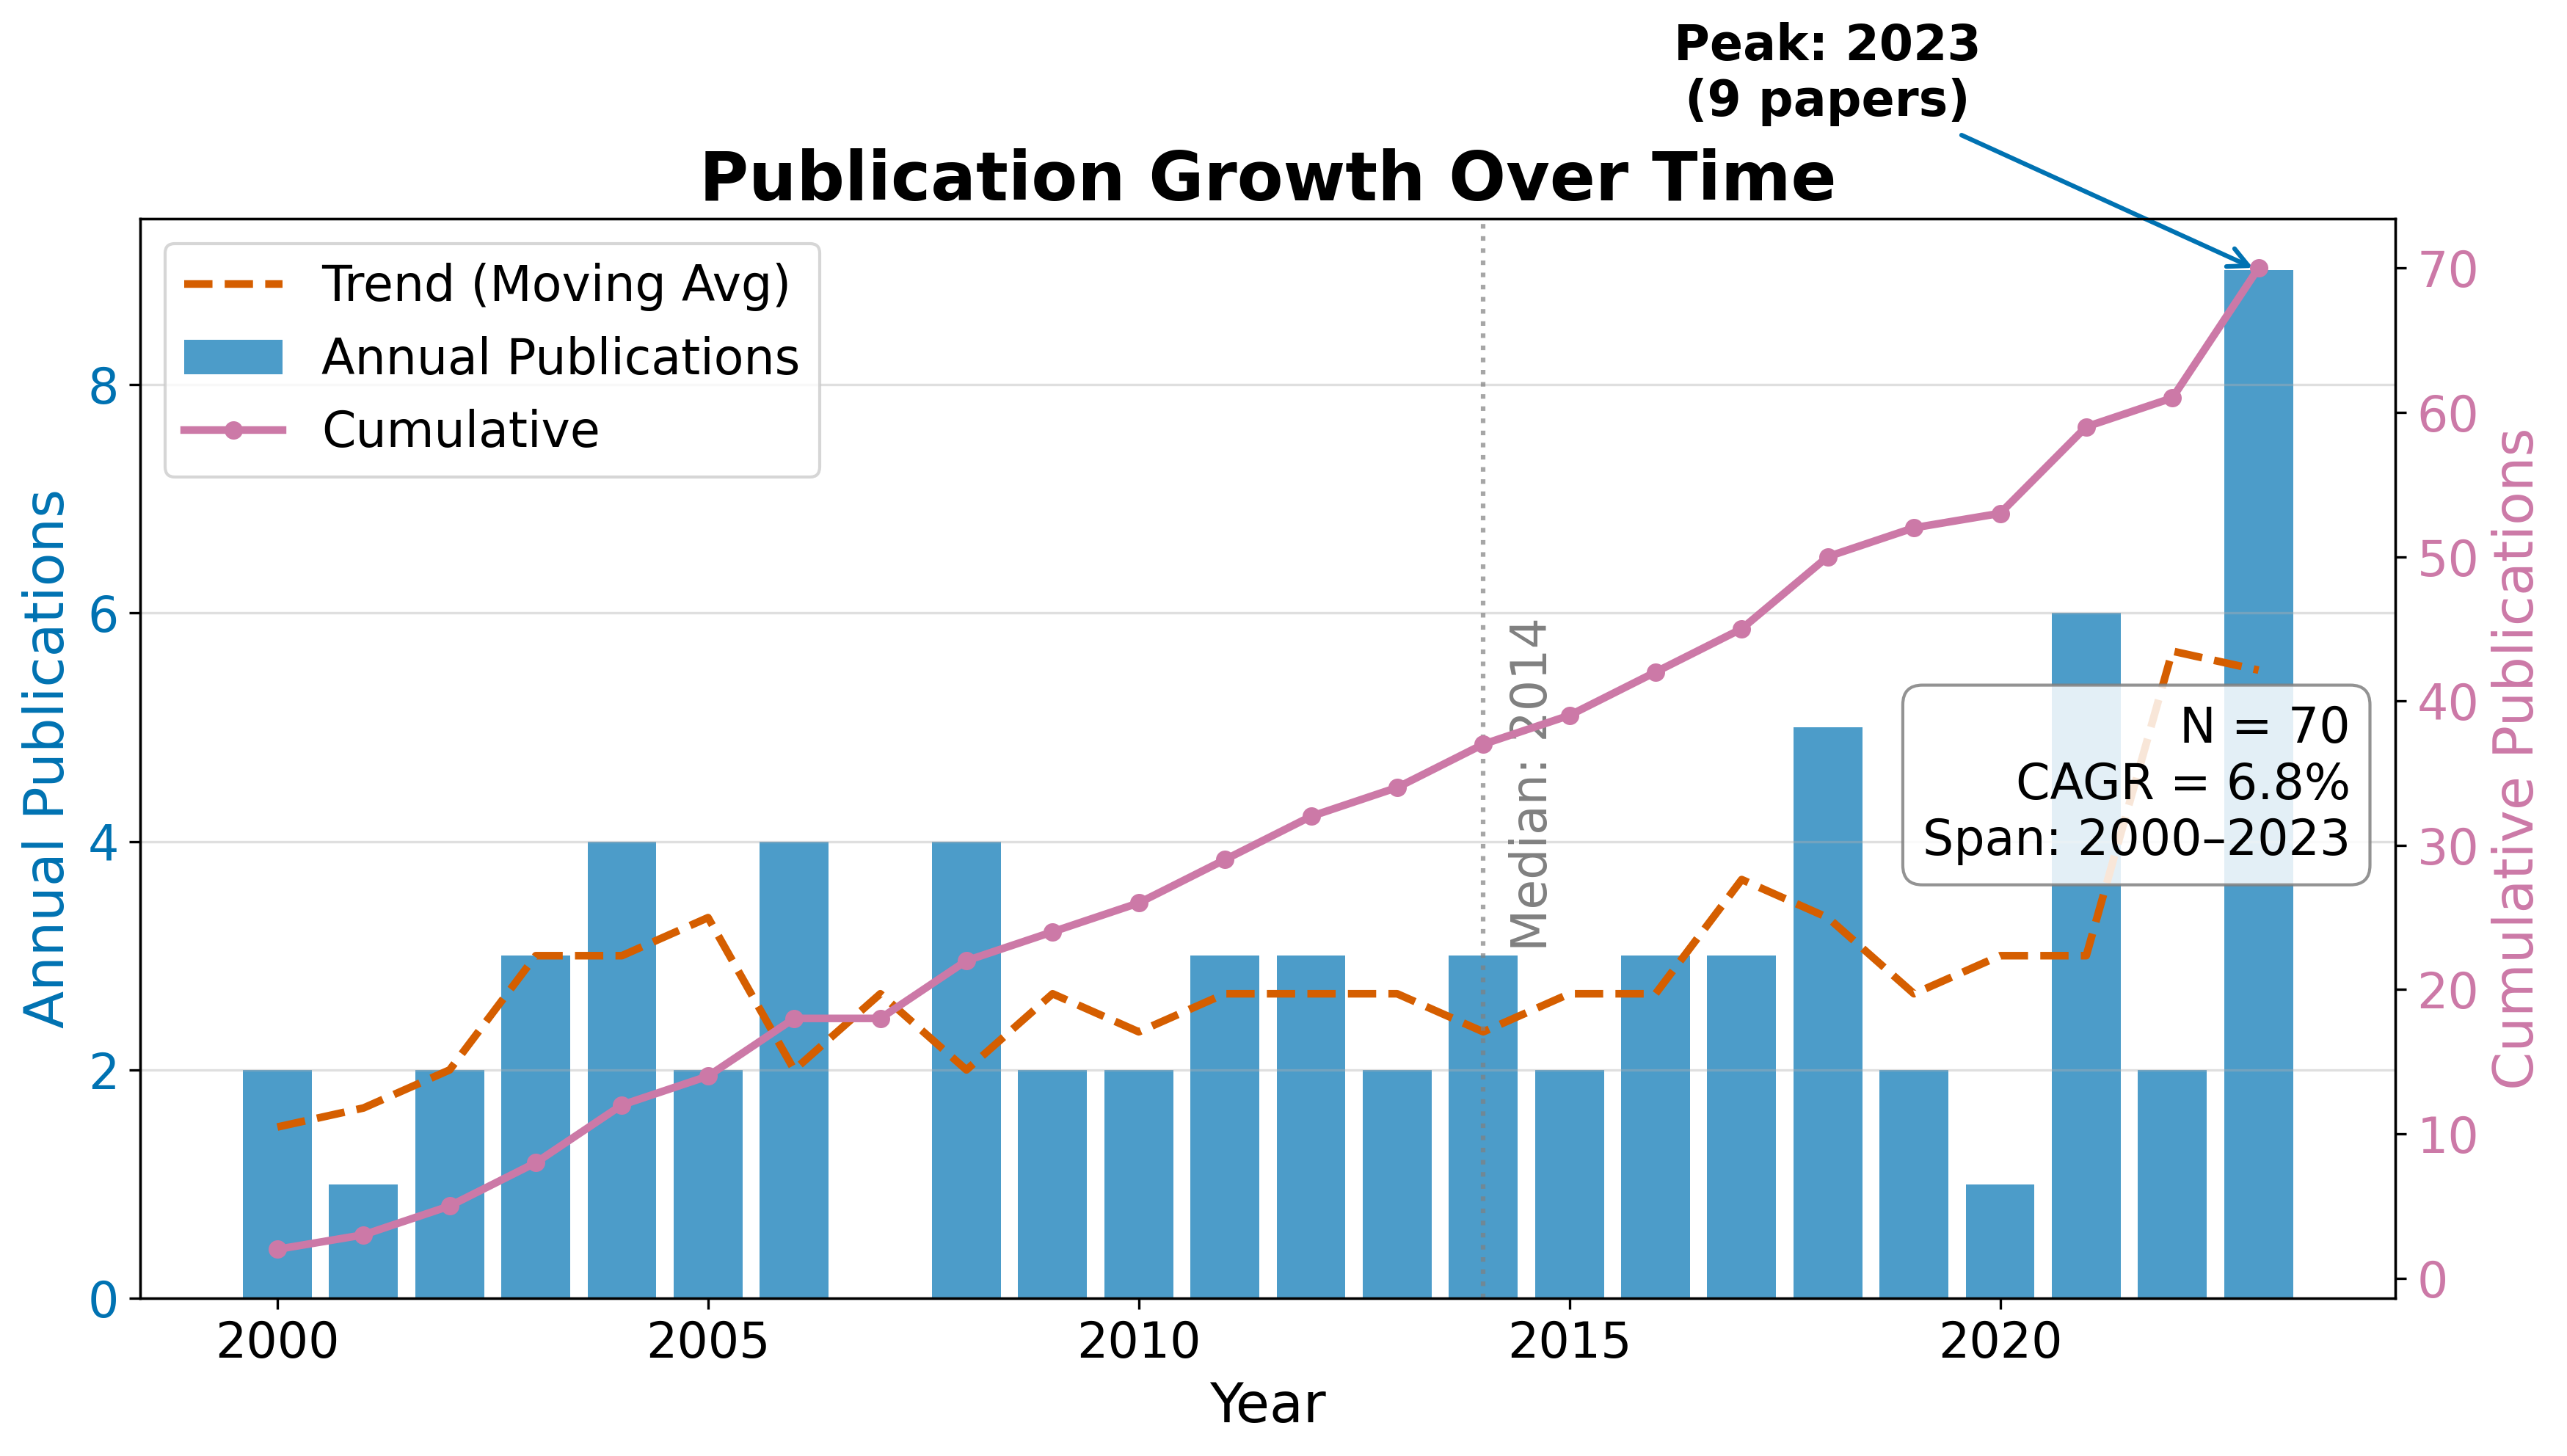
\includegraphics{../figures/growth_curve.png}
\caption{Publication growth curve for \{\{SEARCH\_TERM\_TITLE\}\}.
Annual publication counts (bars) and cumulative total (line) show
sustained growth from \{\{YEAR\_START\}\} through \{\{YEAR\_END\}\},
peaking in \{\{PEAK\_YEAR\}\}.}\label{fig:growth_curve}
\end{figure}

\subsection{RQ1: Field Size and Growth}\label{rq1-field-size-and-growth}

The temporal analysis describes a retained literature slice spanning
\{\{YEAR\_SPAN\}\} years. The compound annual growth rate of
\{\{CAGR\_PCT\}\}\% implies a corpus doubling time of approximately
\{\{DOUBLING\_TIME\}\} years under the configured retrieval and indexing
conditions. The peak year \{\{PEAK\_YEAR\}\} contains
\{\{PEAK\_YEAR\_PUBS\}\} retained records; that count may reflect both
publication activity and delays or differences in source indexing, so it
should not be interpreted as a causal trend without a live coverage
audit.

\textbf{Table 1. Top publication years.}

\{\{YEAR\_COUNT\_TABLE\}\}

\subsection{RQ2: Subfield Composition}\label{rq2-subfield-composition}

Records distribute across the \{\{N\_SUBFIELDS\}\} configured subfields
as shown in Table 2, with \textbf{\{\{TOP\_SUBFIELD\}\}} the largest
bucket at \{\{TOP\_SUBFIELD\_PCT\}\}\% of the classified corpus. The
dominance of \{\{TOP\_SUBFIELD\}\} is a property of the configured
taxonomy and retained corpus. It is not a domain prevalence estimate
without a live, source-backed review and a documented coverage
assessment.

\textbf{Table 2. Subfield distribution.}

\{\{SUBFIELD\_TABLE\}\}

\begin{figure}
\centering
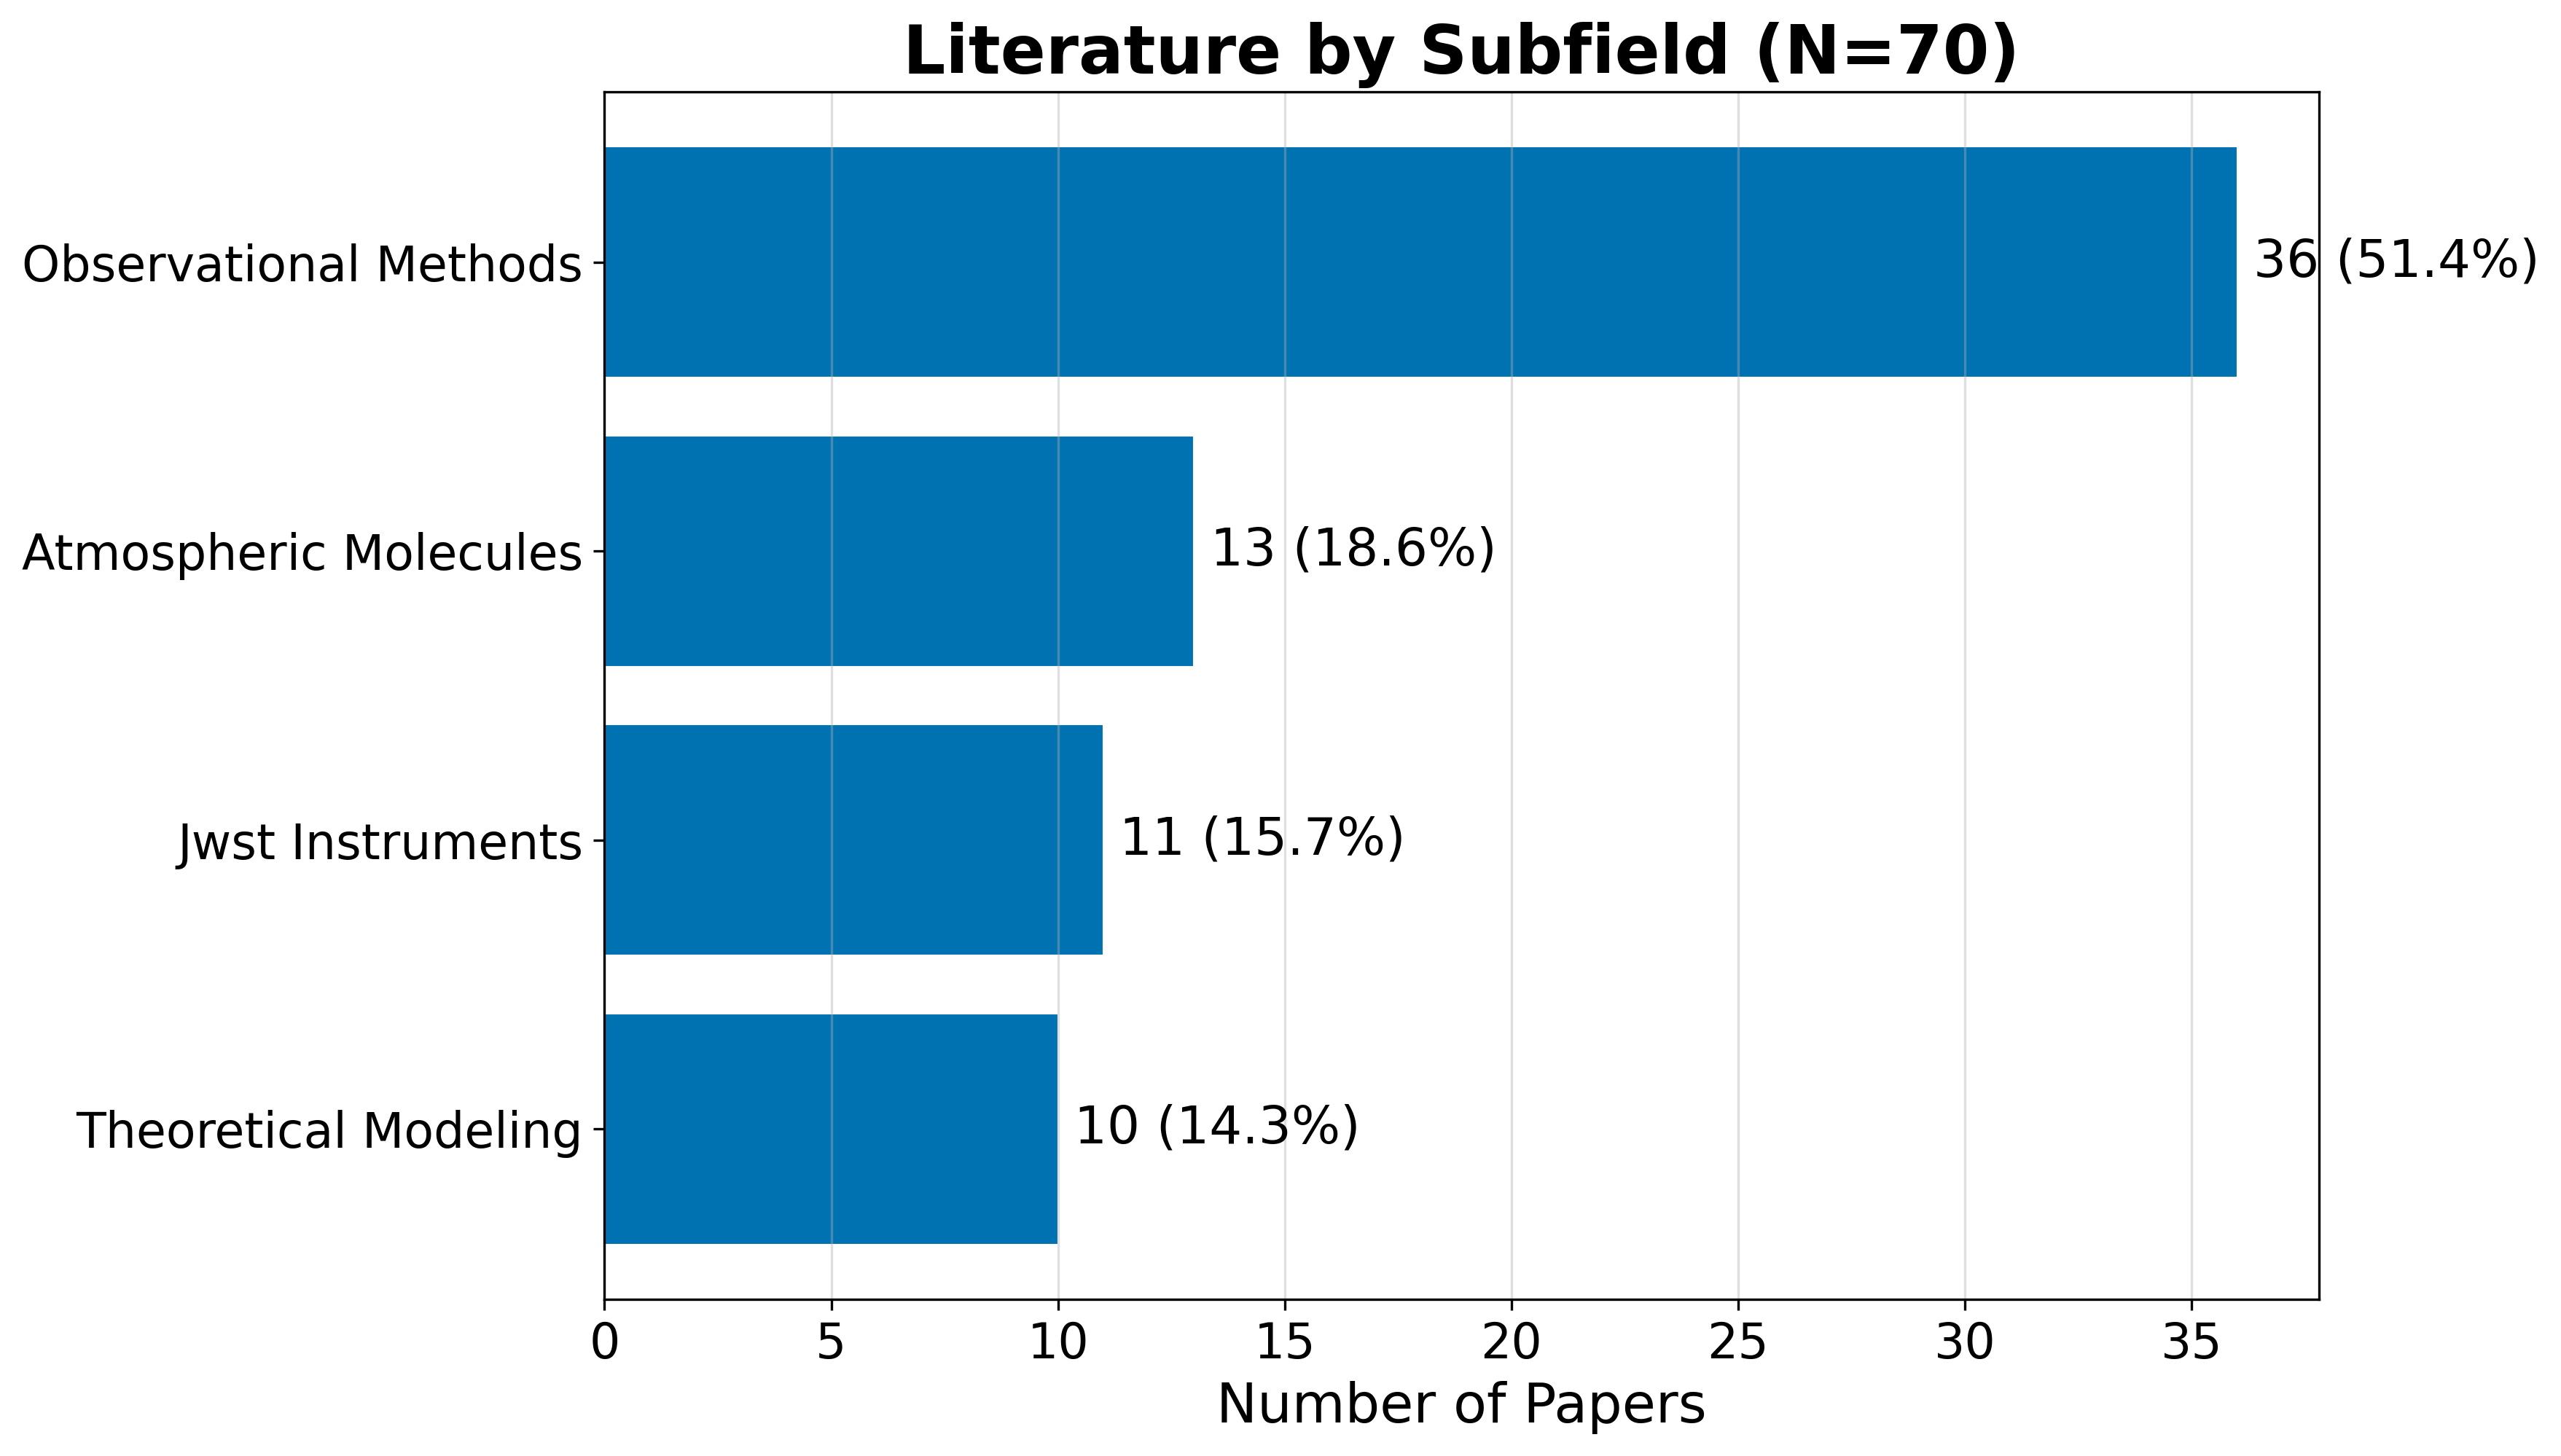
\includegraphics{../figures/field_summary.png}
\caption{Field summary dashboard for \{\{SEARCH\_TERM\_TITLE\}\}. The
dashboard combines corpus size, temporal range, subfield distribution,
and key bibliometric indicators in a single overview
panel.}\label{fig:field_summary}
\end{figure}

\begin{figure}
\centering
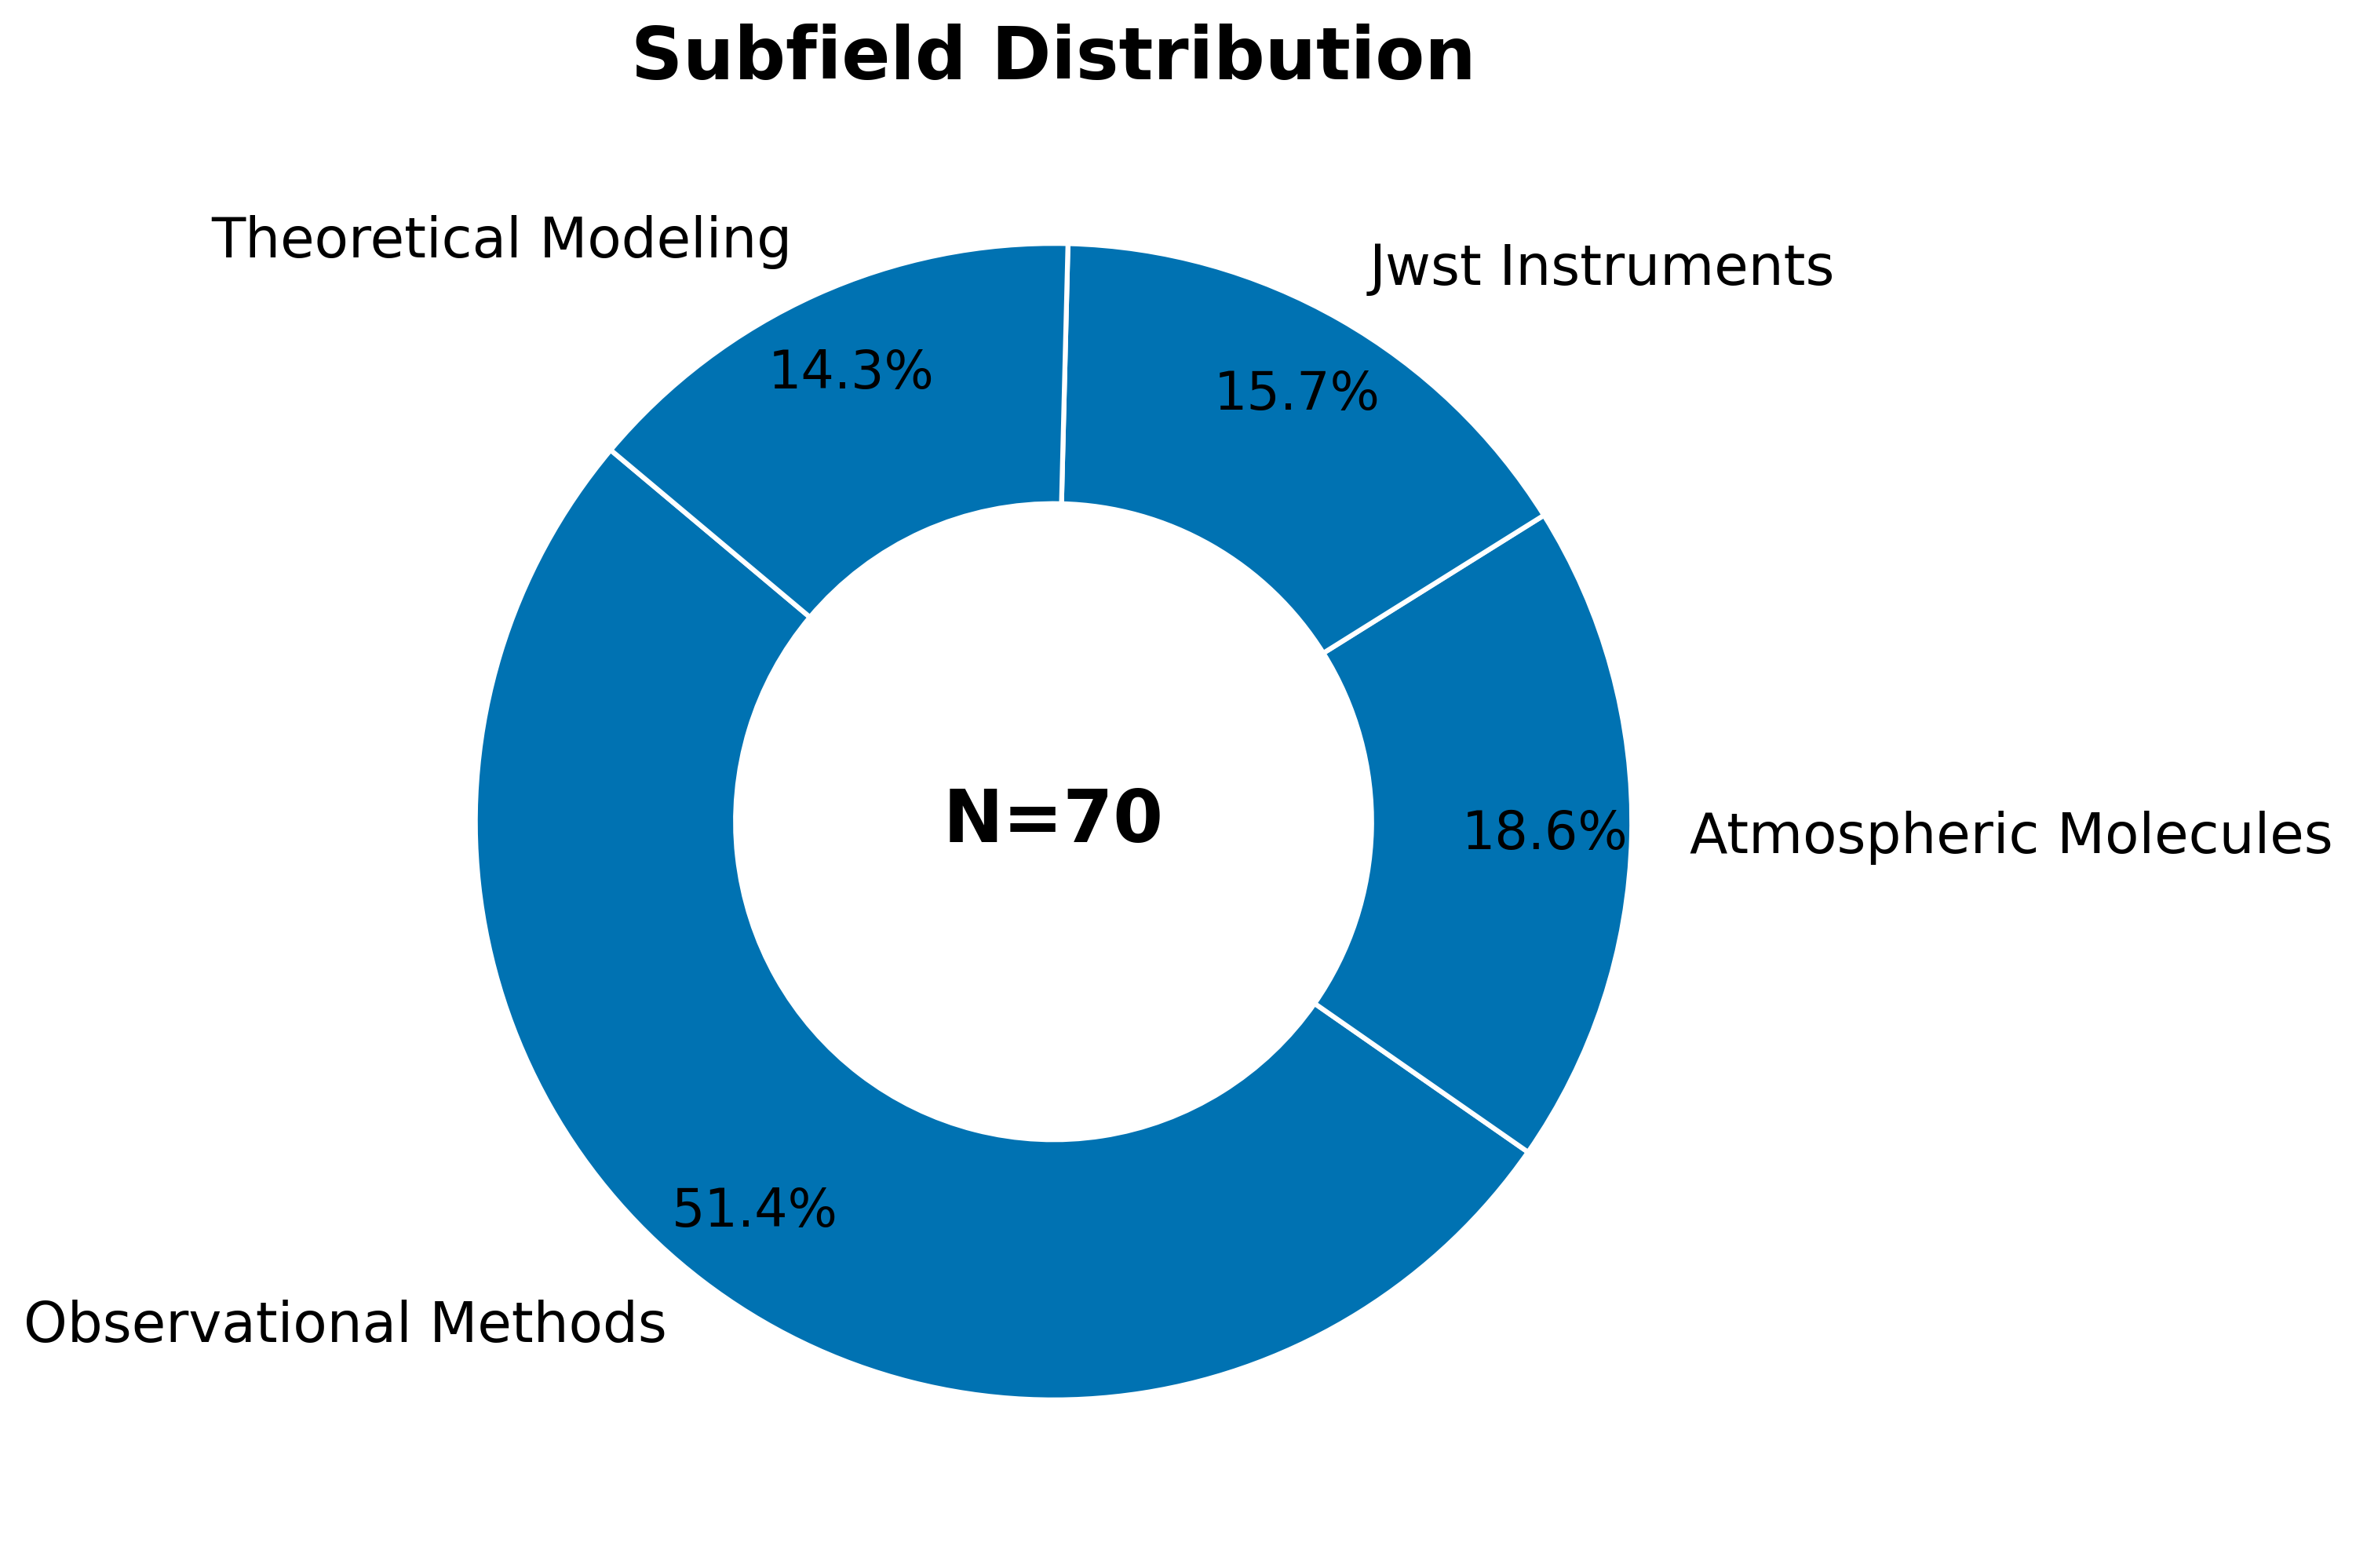
\includegraphics{../figures/subfield_distribution.png}
\caption{Subfield distribution for \{\{SEARCH\_TERM\_TITLE\}\}. The
\{\{N\_SUBFIELDS\}\}-bucket taxonomy shows the relative weight of each
configured sub-area, with \{\{TOP\_SUBFIELD\}\} dominant at
\{\{TOP\_SUBFIELD\_PCT\}\}\%.}\label{fig:subfield_distribution}
\end{figure}

\newpage

\begin{figure}
\centering
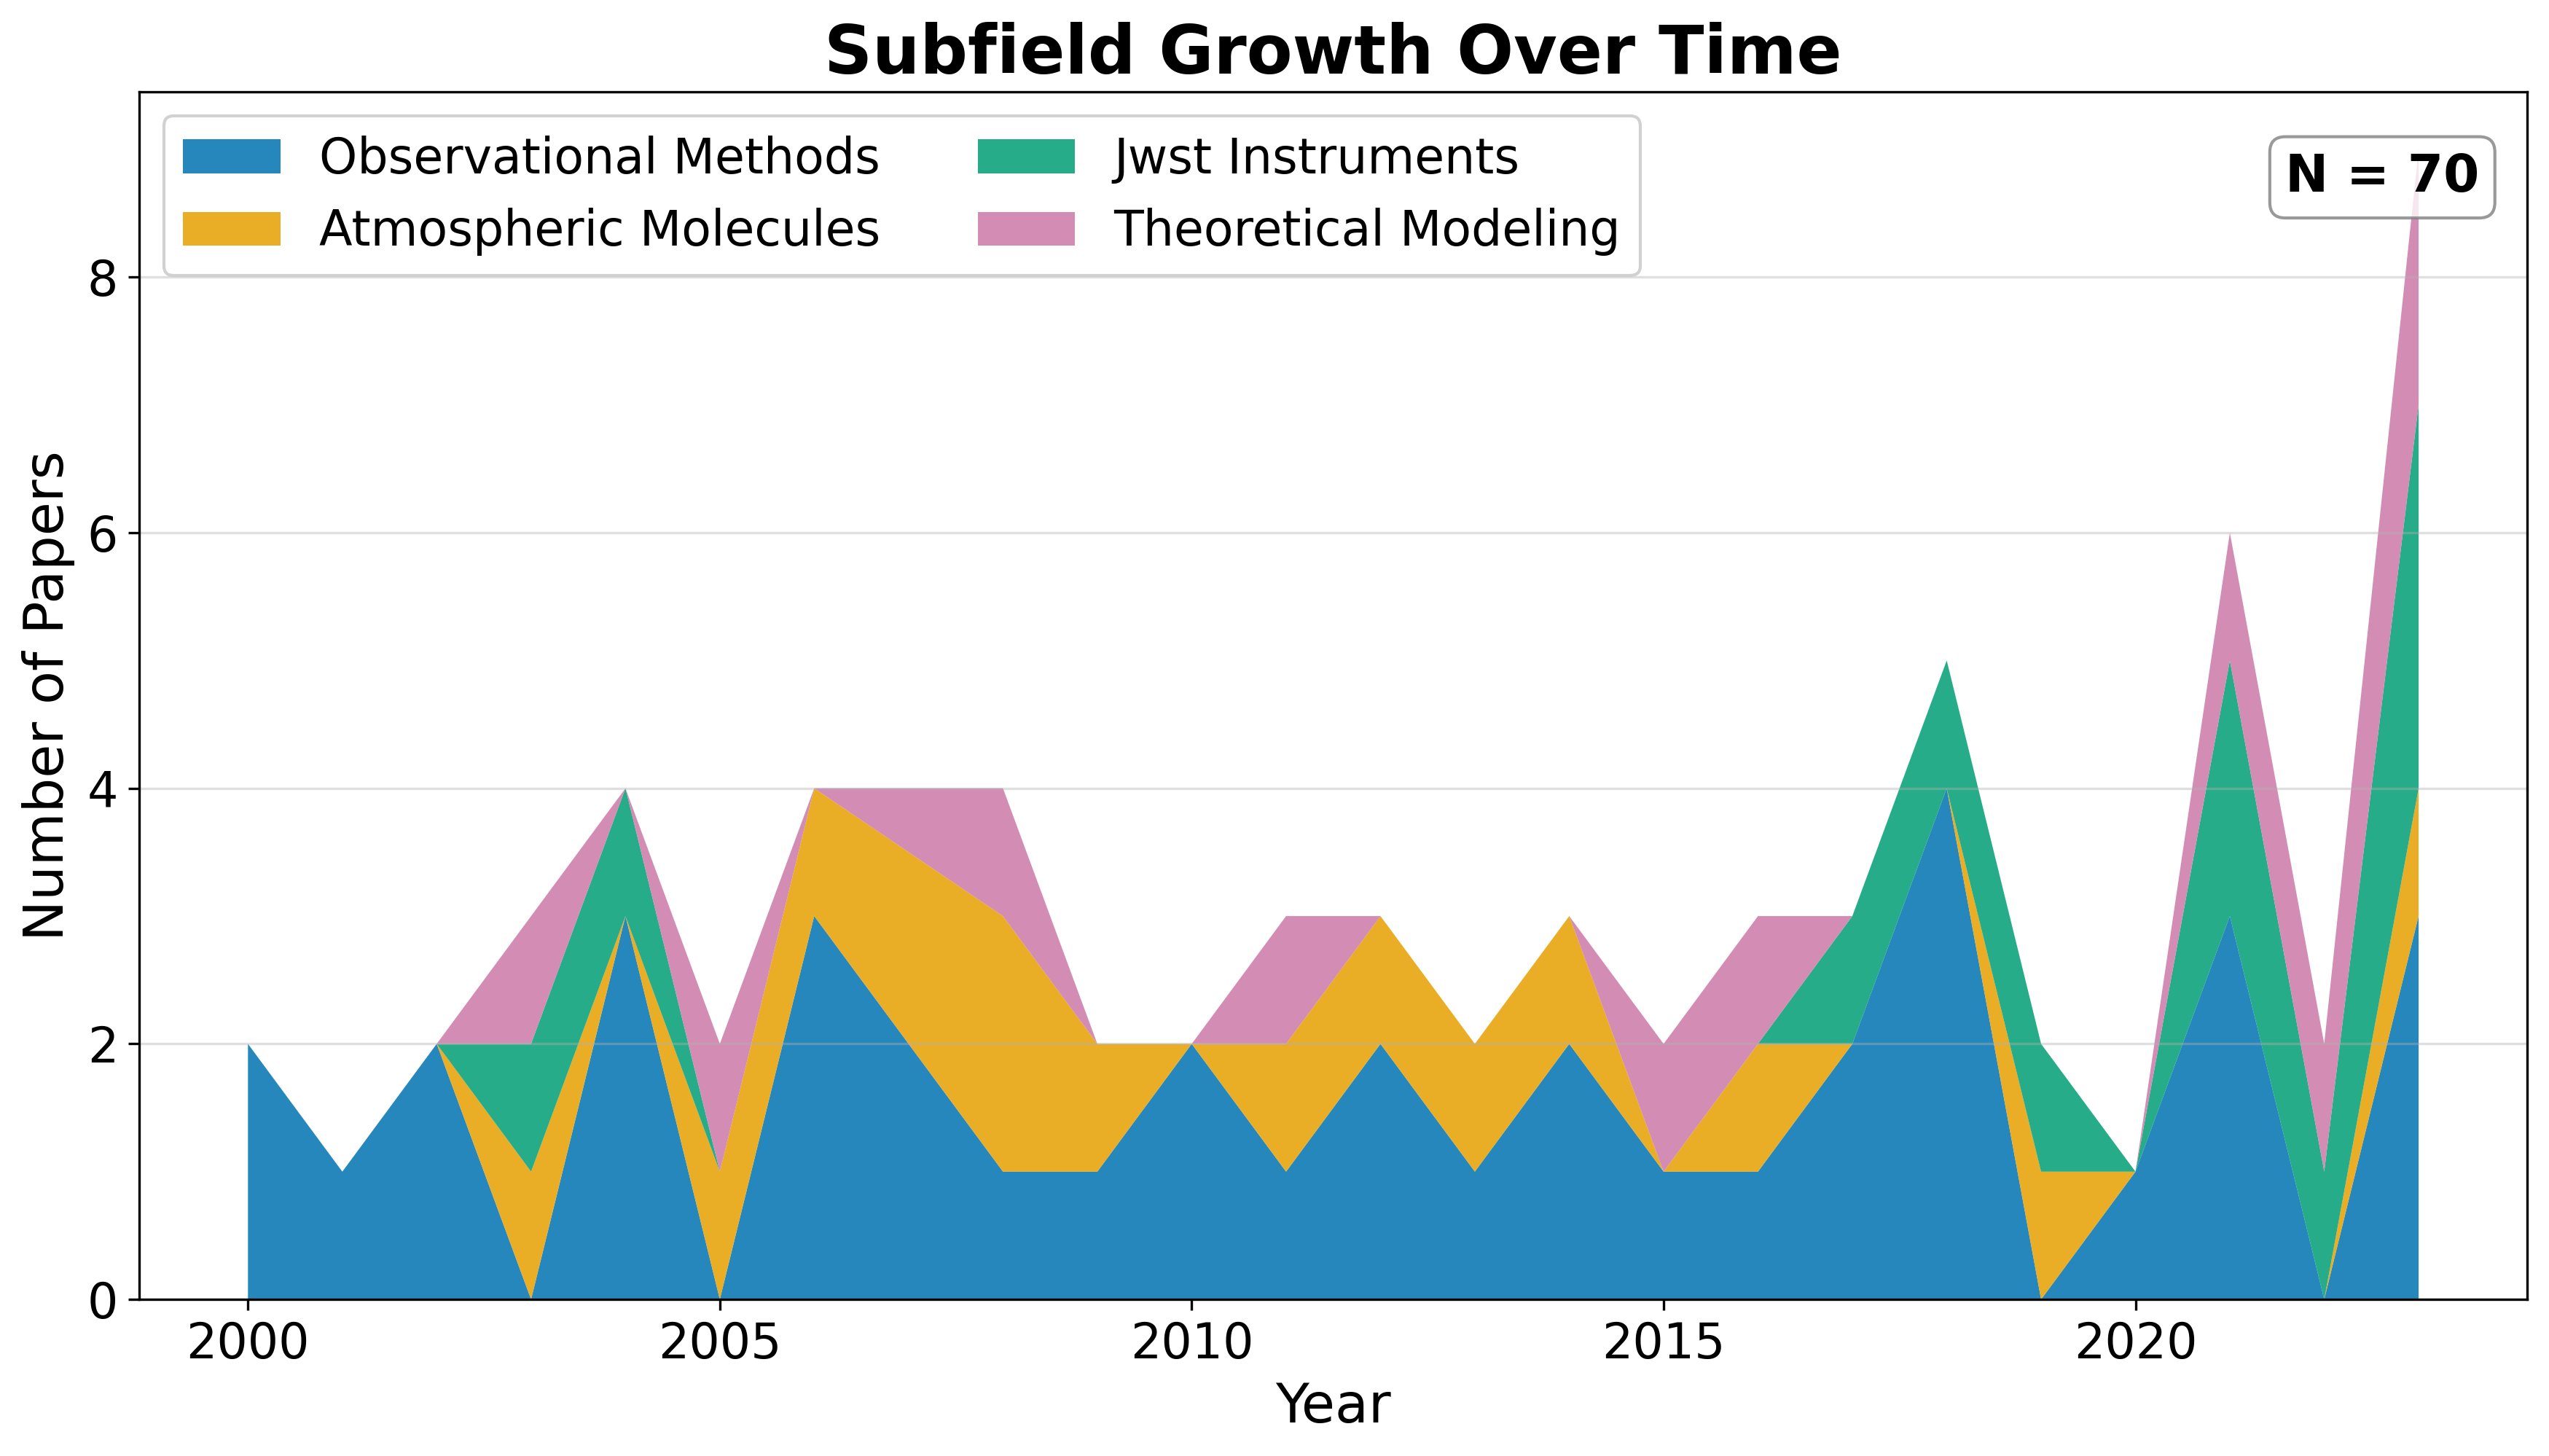
\includegraphics{../figures/subfield_timeline.png}
\caption{Subfield timeline for \{\{SEARCH\_TERM\_TITLE\}\}. Stacked
annual publication counts by subfield show how each sub-area has evolved
over time, revealing emerging and declining research
threads.}\label{fig:subfield_timeline}
\end{figure}

\subsection{Identifier and Full-Text
Coverage}\label{identifier-and-full-text-coverage}

The corpus has measurable identifier coverage: \{\{DOI\_COUNT\}\} of
\{\{CORPUS\_SIZE\}\} records (\{\{PCT\_WITH\_DOI\}\}\%) carry DOIs,
supporting cross-engine de-duplication. OpenAlex IDs are present for
\{\{OPENALEX\_ID\_COUNT\}\} records. Abstract coverage stands at
\{\{ABSTRACT\_COVERAGE\_PCT\}\}\% (\{\{ABSTRACT\_COUNT\}\} records),
which limits the text analytics to that subset. Open-access status is
confirmed for \{\{OA\_PCT\}\}\% of records, and
\{\{PDF\_AVAIL\_PCT\}\}\% have a direct PDF link.

\subsection{Descriptive Bibliometrics}\label{descriptive-bibliometrics}

The corpus spans \{\{UNIQUE\_AUTHORS\}\} unique authors across
\{\{CORPUS\_SIZE\}\} papers, yielding a mean of
\{\{PAPERS\_PER\_AUTHOR\_MEAN\}\} papers per author. Citation counts
range from zero to \{\{CITATION\_MAX\}\} (mean \{\{CITATION\_MEAN\}\},
median \{\{CITATION\_MEDIAN\}\}), with a total of
\{\{CITATION\_TOTAL\}\} citations across the corpus. The Gini
coefficient of citation concentration is \{\{GINI\_COEFFICIENT\}\}. This
statistic describes concentration within the retained corpus and should
not be generalized to citation behavior in the field.

\textbf{Table 3. Citation count distribution.}

\{\{CITATION\_DIST\_TABLE\}\}

\begin{figure}
\centering
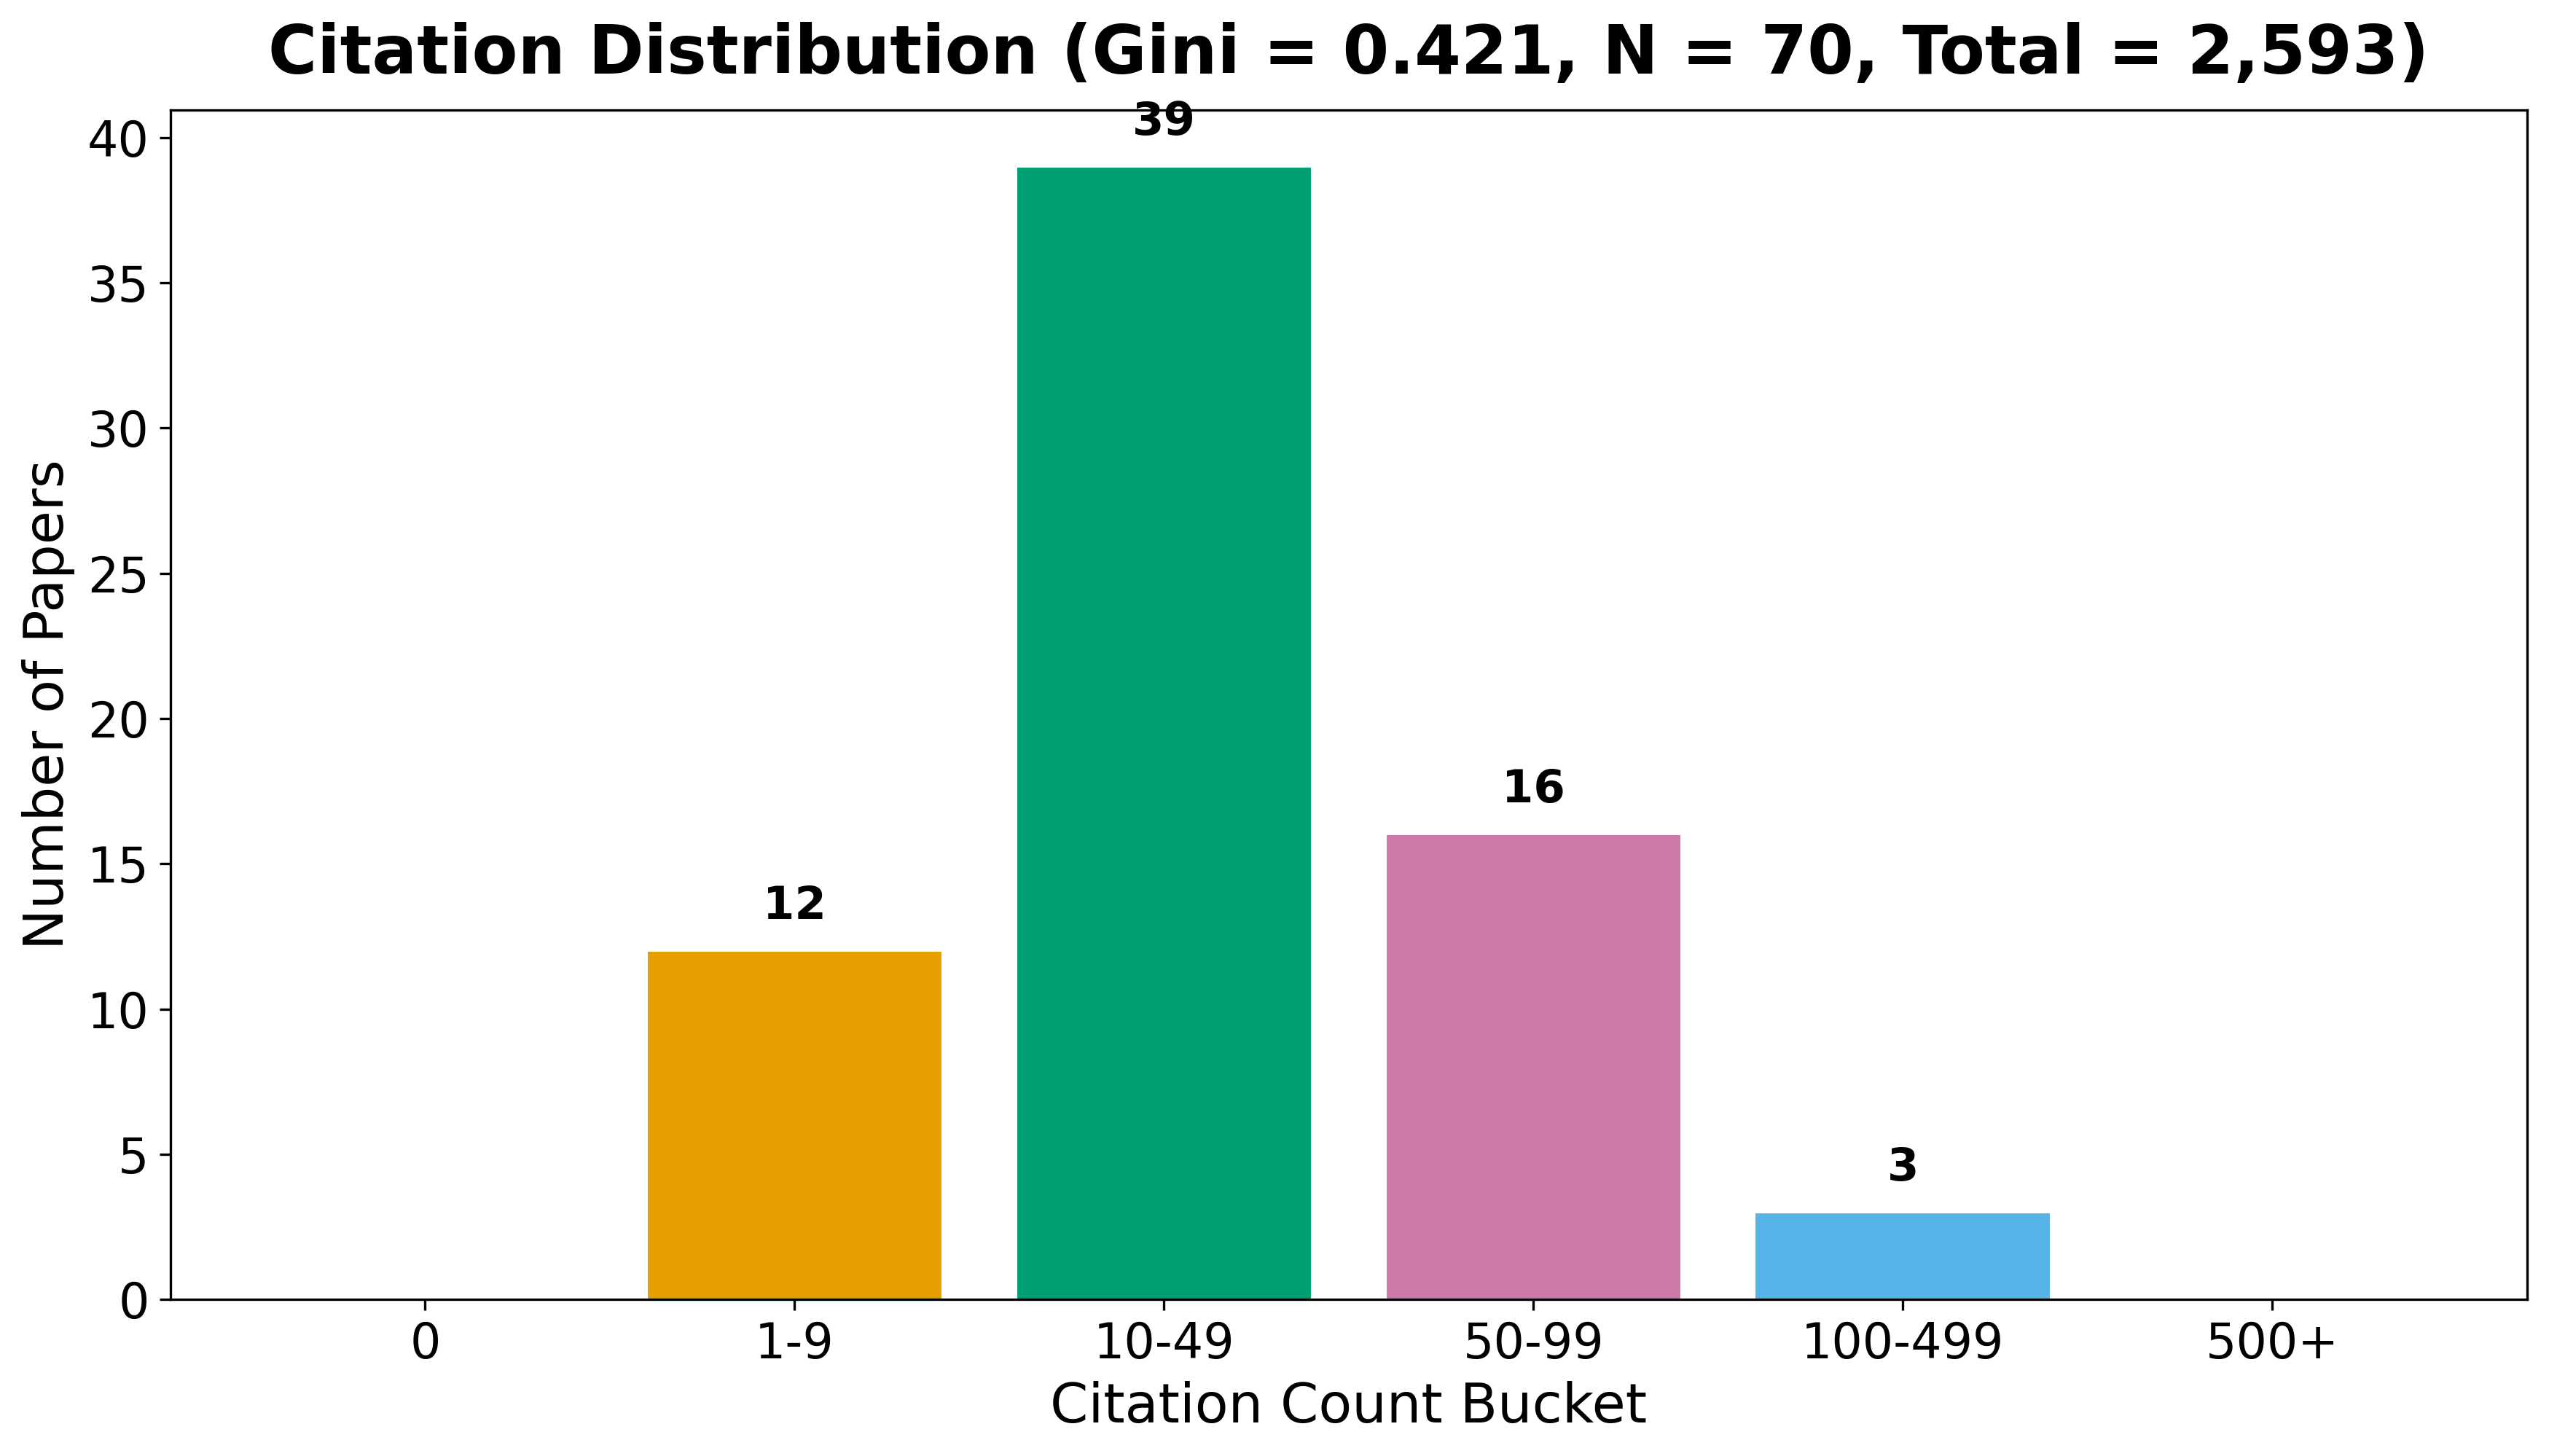
\includegraphics{../figures/citation_distribution.png}
\caption{Citation distribution for \{\{SEARCH\_TERM\_TITLE\}\}. The
histogram shows the number of papers in each citation-count bucket, with
the Gini coefficient annotated. The distribution is a descriptive
property of the retained corpus.}\label{fig:citation_distribution}
\end{figure}

\newpage

\textbf{Table 4. Top publication venues.}

\{\{TOP\_VENUES\_TABLE\}\}

\begin{figure}
\centering
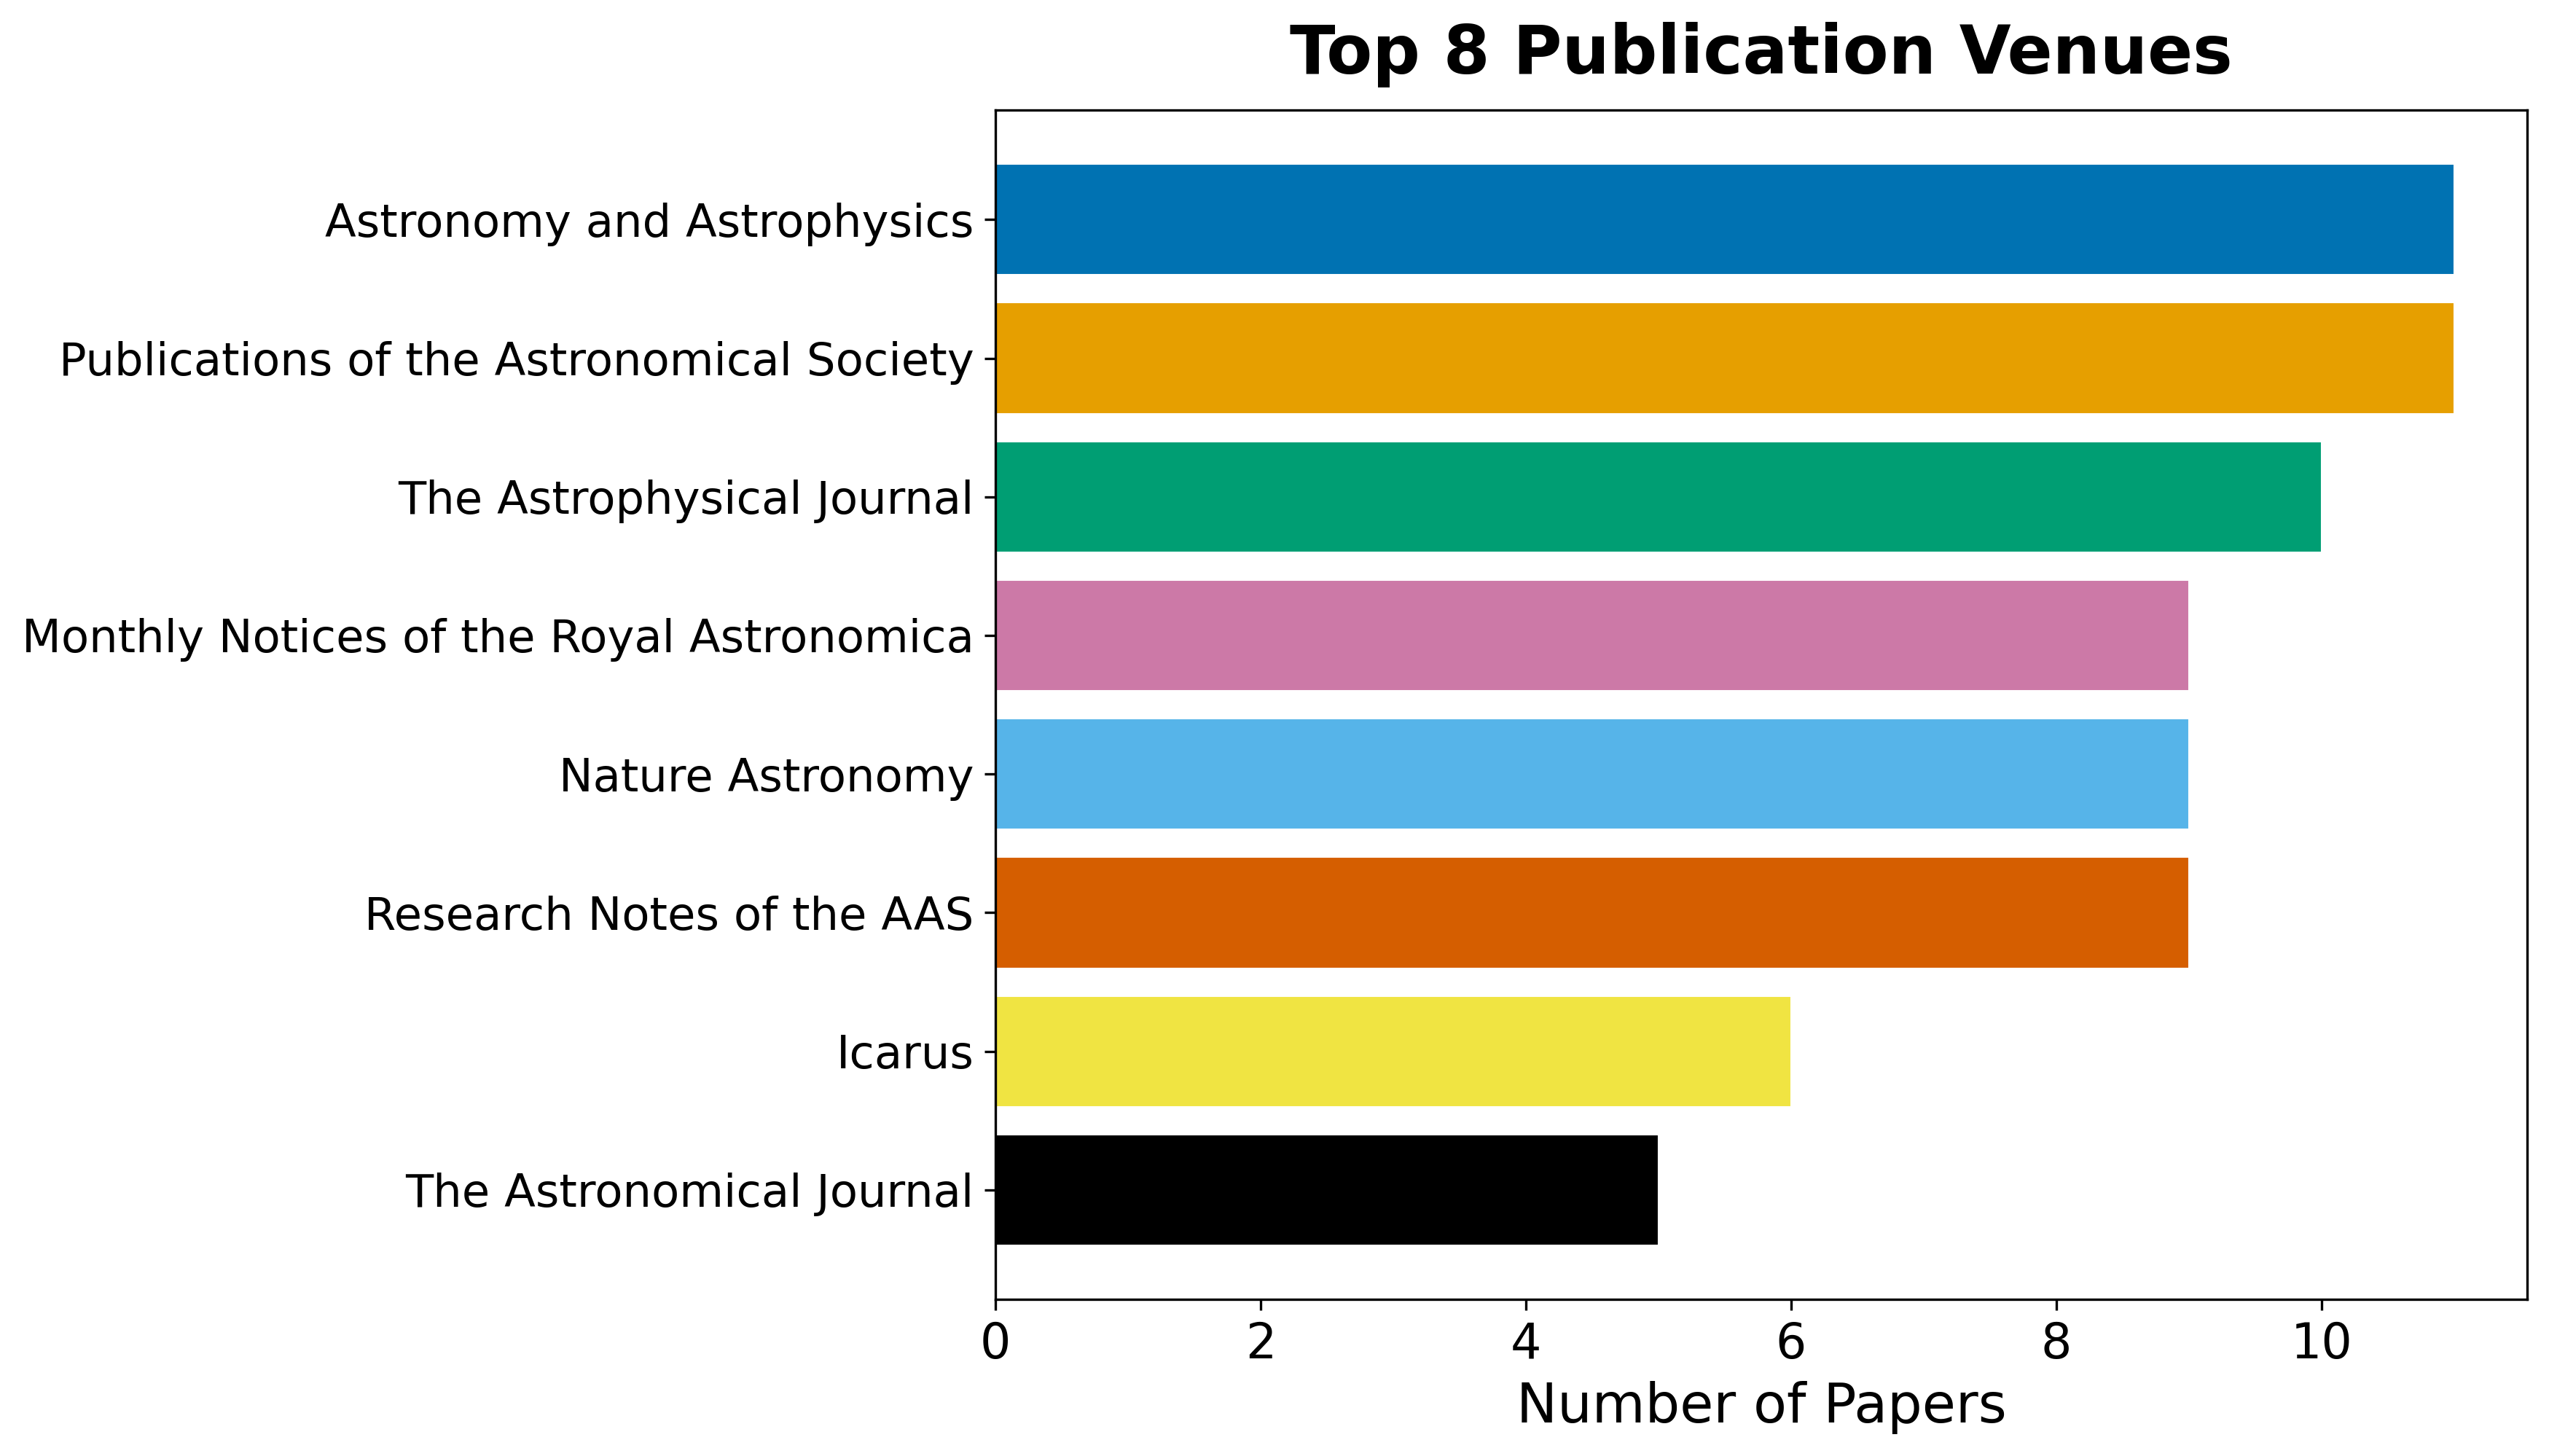
\includegraphics{../figures/top_venues.png}
\caption{Top publication venues for \{\{SEARCH\_TERM\_TITLE\}\}. The
horizontal bar chart shows the venues with the most retained records; it
describes this corpus rather than the complete
field.}\label{fig:top_venues}
\end{figure}

\textbf{Table 5. Top authors by publication count.}

\{\{TOP\_AUTHORS\_TABLE\}\}

\begin{figure}
\centering
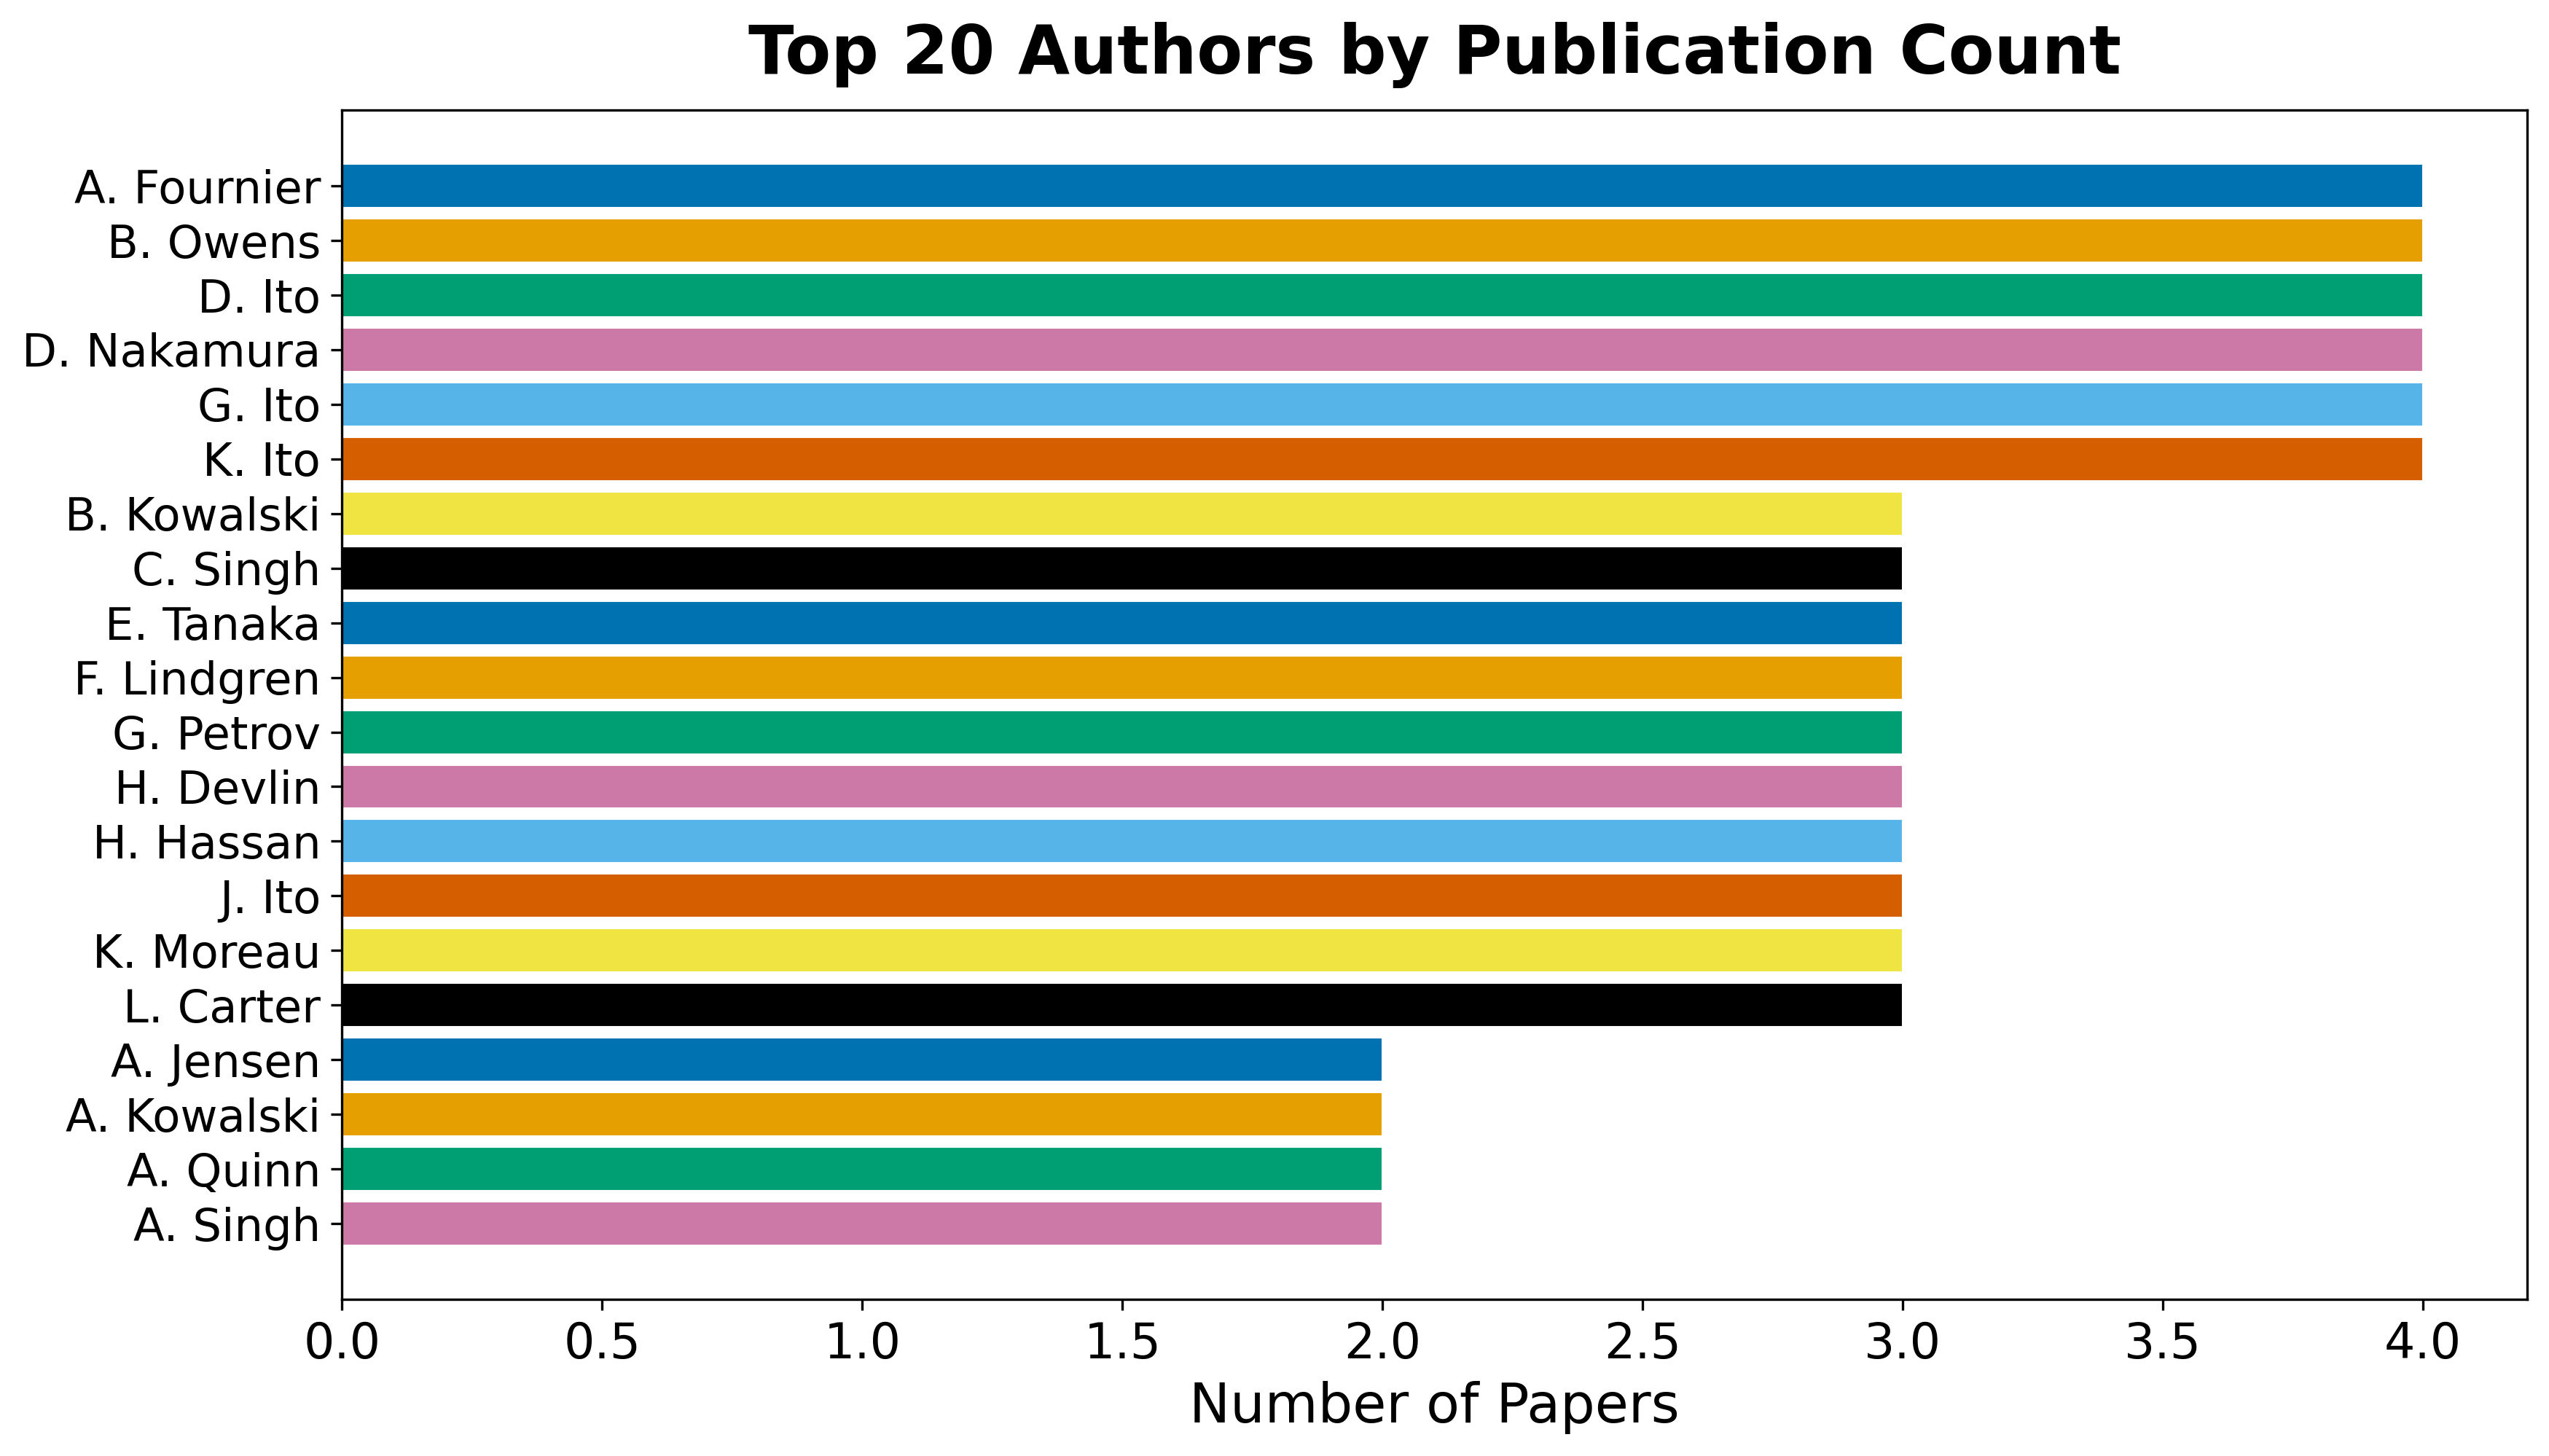
\includegraphics{../figures/author_productivity.png}
\caption{Author productivity for \{\{SEARCH\_TERM\_TITLE\}\}. The
horizontal bar chart shows authors with the most retained records; names
and counts depend on source coverage and
deduplication.}\label{fig:author_productivity}
\end{figure}

\newpage

\section{Results: Subfield Structure}\label{results-subfield-structure}

The subfield taxonomy is configuration-owned. For this instance it
contains \{\{N\_SUBFIELDS\}\} buckets (\{\{SUBFIELD\_LIST\}\}), and each
retained record is assigned using the documented keyword precedence. The
resulting distribution is descriptive of the retrieval slice and should
not be read as a prevalence estimate for the complete field.

\subsection{Per-subfield
characterization}\label{per-subfield-characterization}

The configured buckets distinguish observational methods, atmospheric
molecules, JWST instrumentation, and theoretical modeling. A fork may
add or rename buckets without changing the analysis code; the taxonomy,
keyword lists, and phase relevance should be reviewed together.

The largest bucket is \textbf{\{\{TOP\_SUBFIELD\}\}} at
\{\{TOP\_SUBFIELD\_PCT\}\}\%. Table 2 and the generated subfield
artifacts provide the counts and annual breakdown. Where the fixture
corpus is used, these values demonstrate classification behavior only
and are marked synthetic in the evidence registry.

\{\{SUBFIELD\_TABLE\}\}

\newpage

\section{Results: Language, Topics, and
Embeddings}\label{results-language-topics-and-embeddings}

\subsection{RQ3: Topical and Linguistic
Structure}\label{rq3-topical-and-linguistic-structure}

Text analysis operates over titles, abstracts, and (when available) full
text. A TF-IDF representation over a
\{\{NUM\_VOCAB\_FEATURES\}\}-feature vocabulary feeds non-negative
matrix factorization, which extracts \{\{NUM\_TOPICS\}\} latent topics
cross-cutting the subfield taxonomy. The top vocabulary terms are:
\{\{TOP\_VOCAB\_TERMS\}\}.

\textbf{Table 3. NMF topics extracted from the corpus.}

\{\{TOPIC\_TABLE\}\}

The topic labels are computed from the retained corpus and are not
hand-assigned. Their interpretation should be checked against the
generated topic-term weights and the configured subfield taxonomy;
fixture-derived topics describe synthetic text patterns, not the
scientific field.

\begin{figure}
\centering
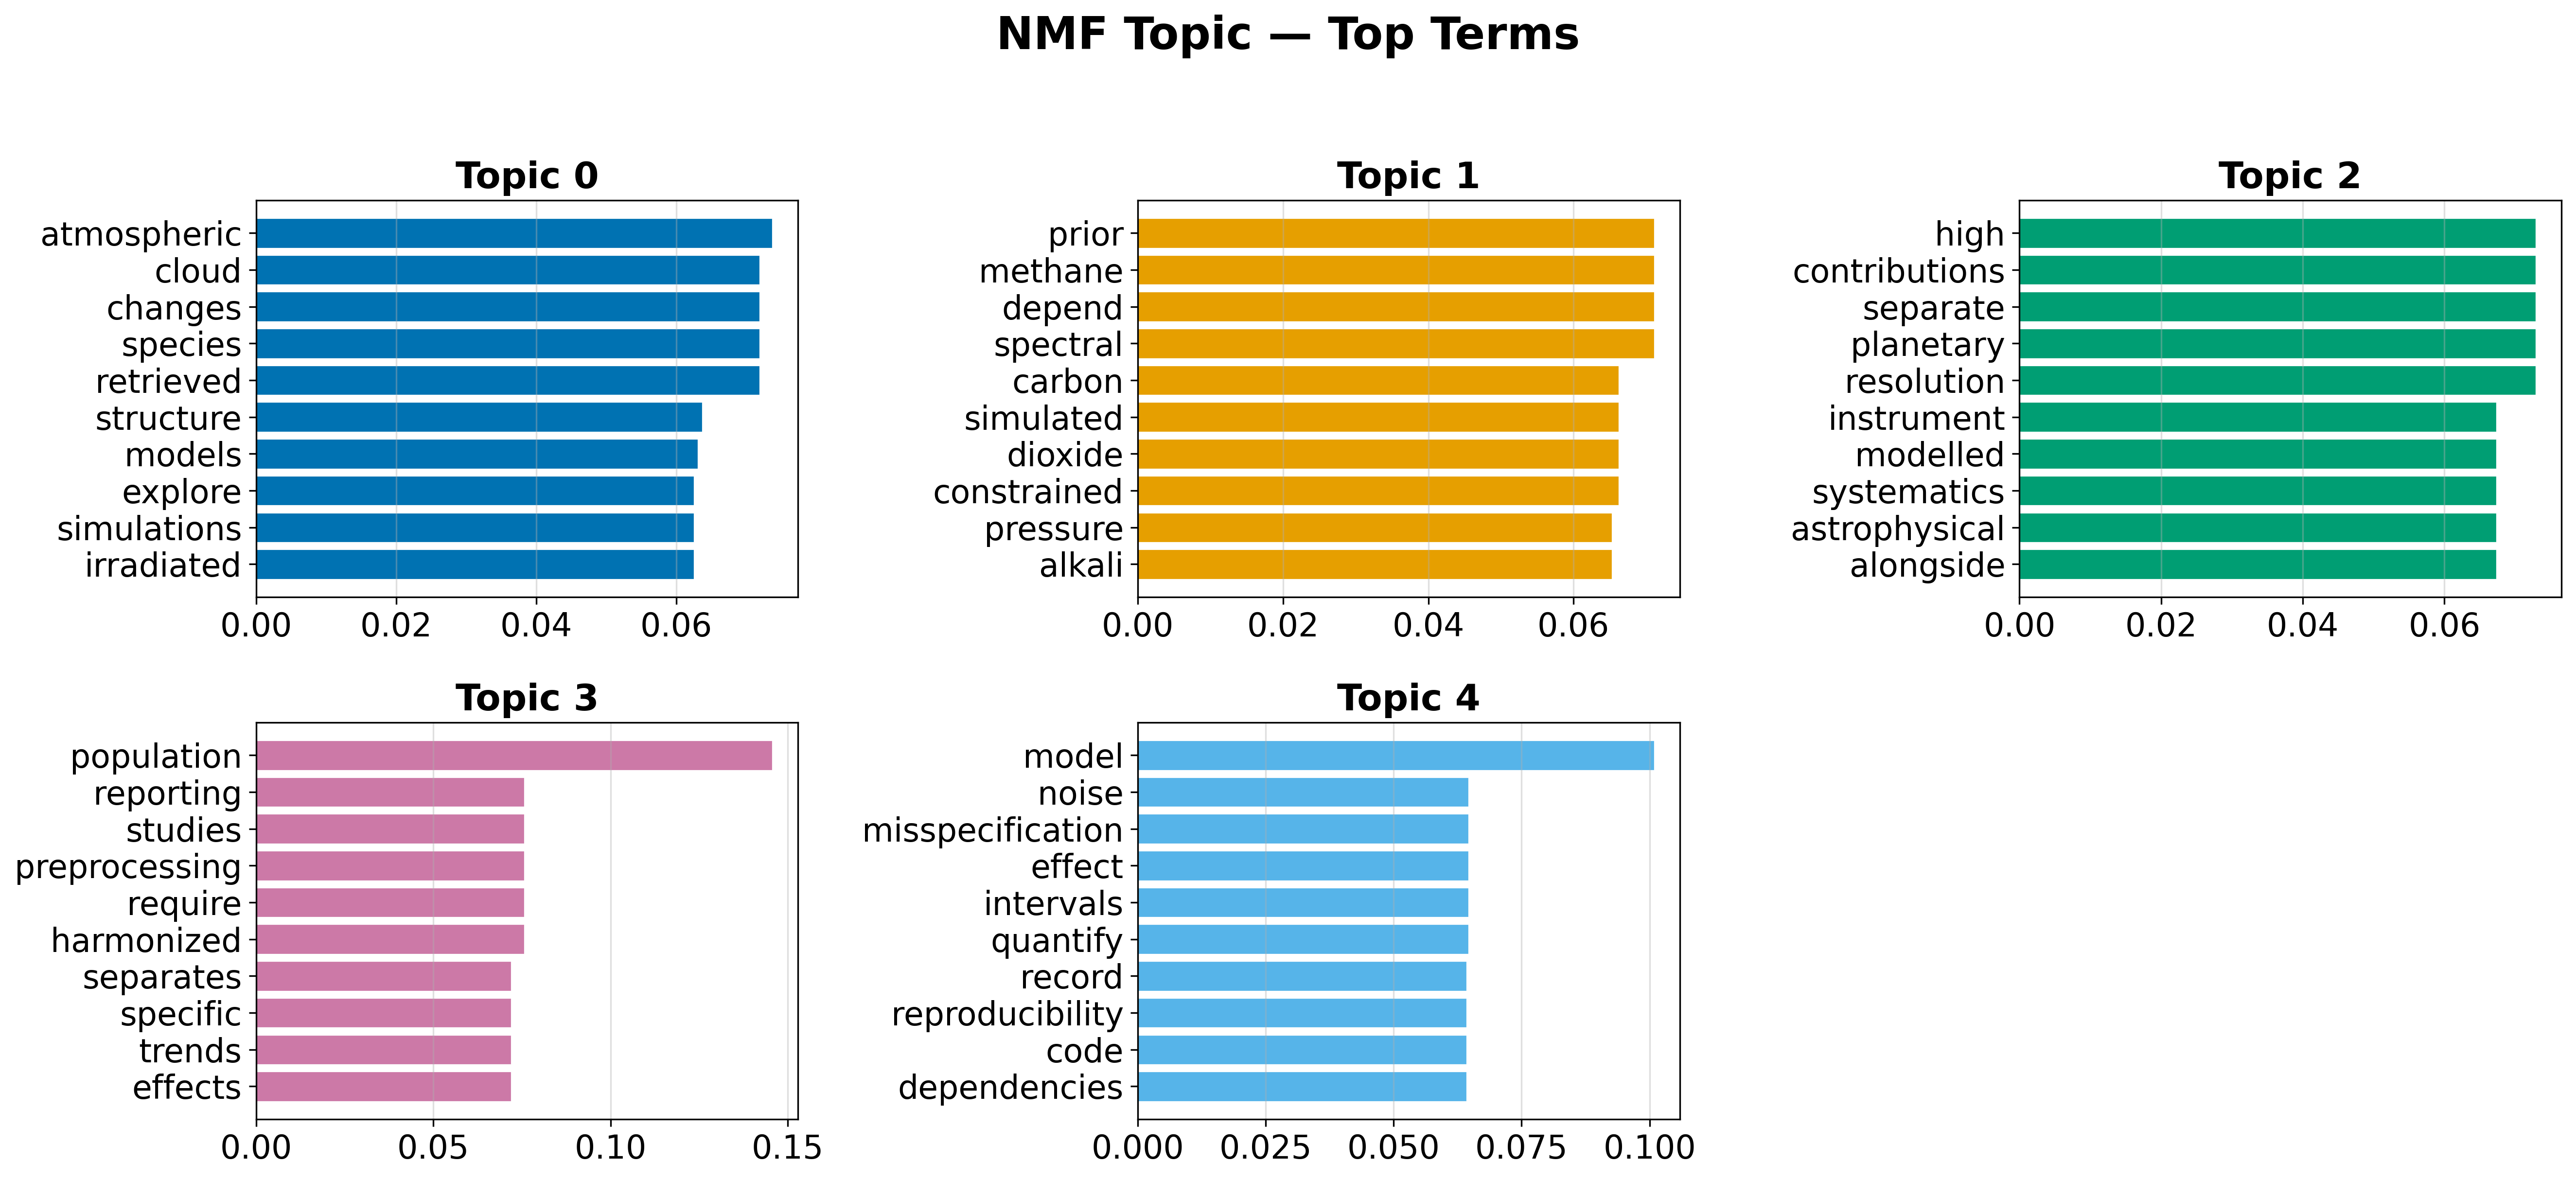
\includegraphics{../figures/topic_term_bars.png}
\caption{Topic-term bar charts for \{\{SEARCH\_TERM\_TITLE\}\}. Each
panel shows the top weighted terms for one of \{\{NUM\_TOPICS\}\} NMF
topics, with bar length proportional to the topic-term weight in the
\(\mathbf{H}\) matrix.}\label{fig:topic_term_bars}
\end{figure}

\subsection{Document Embeddings}\label{document-embeddings}

Offline deterministic embeddings (TF-IDF followed by truncated SVD)
place every document in a shared 50-dimensional vector space. Embedding
the same text twice yields identical vectors, so the derived similarity
matrix, nearest-neighbour lists, clusters, and two-dimensional
projection are all reproducible.

\begin{figure}
\centering
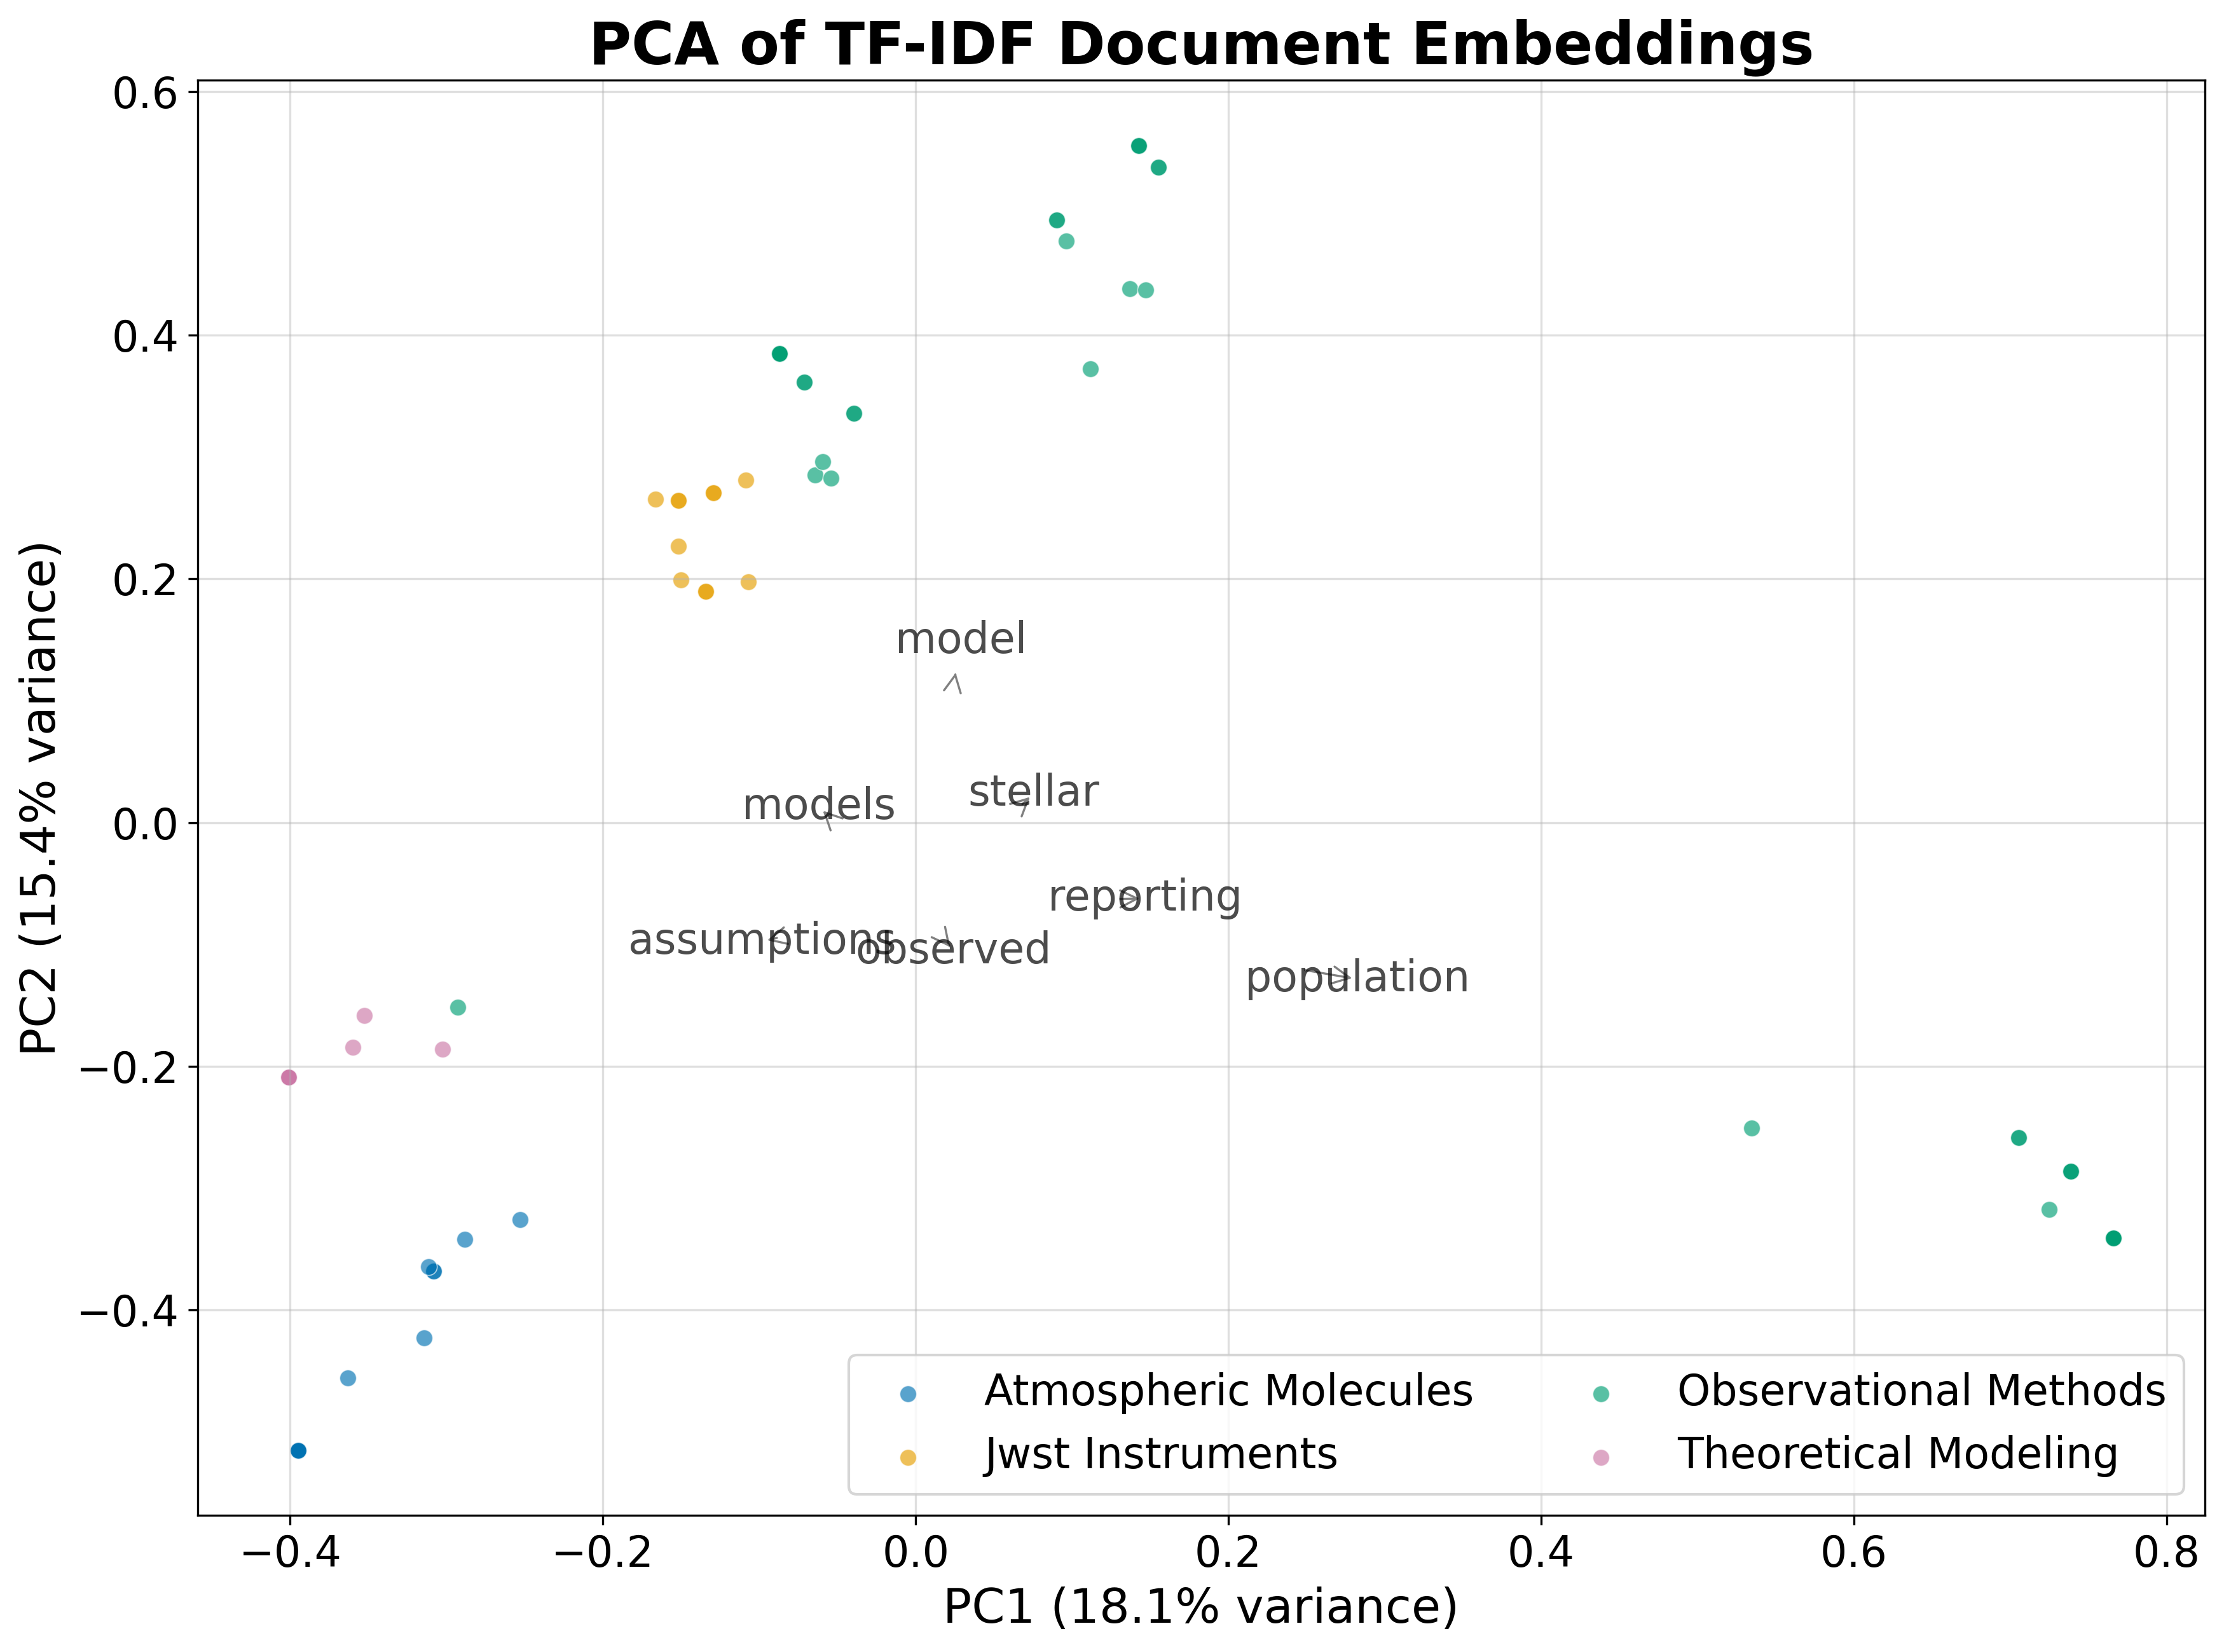
\includegraphics{../figures/pca_embeddings.png}
\caption{PCA projection of document embeddings for
\{\{SEARCH\_TERM\_TITLE\}\}. Each point represents one document
projected onto the first two principal components of the TF-IDF/SVD
embedding. Colours indicate subfield assignment, showing how the topical
geography relates to the keyword taxonomy.}\label{fig:pca_embeddings}
\end{figure}

\begin{figure}
\centering
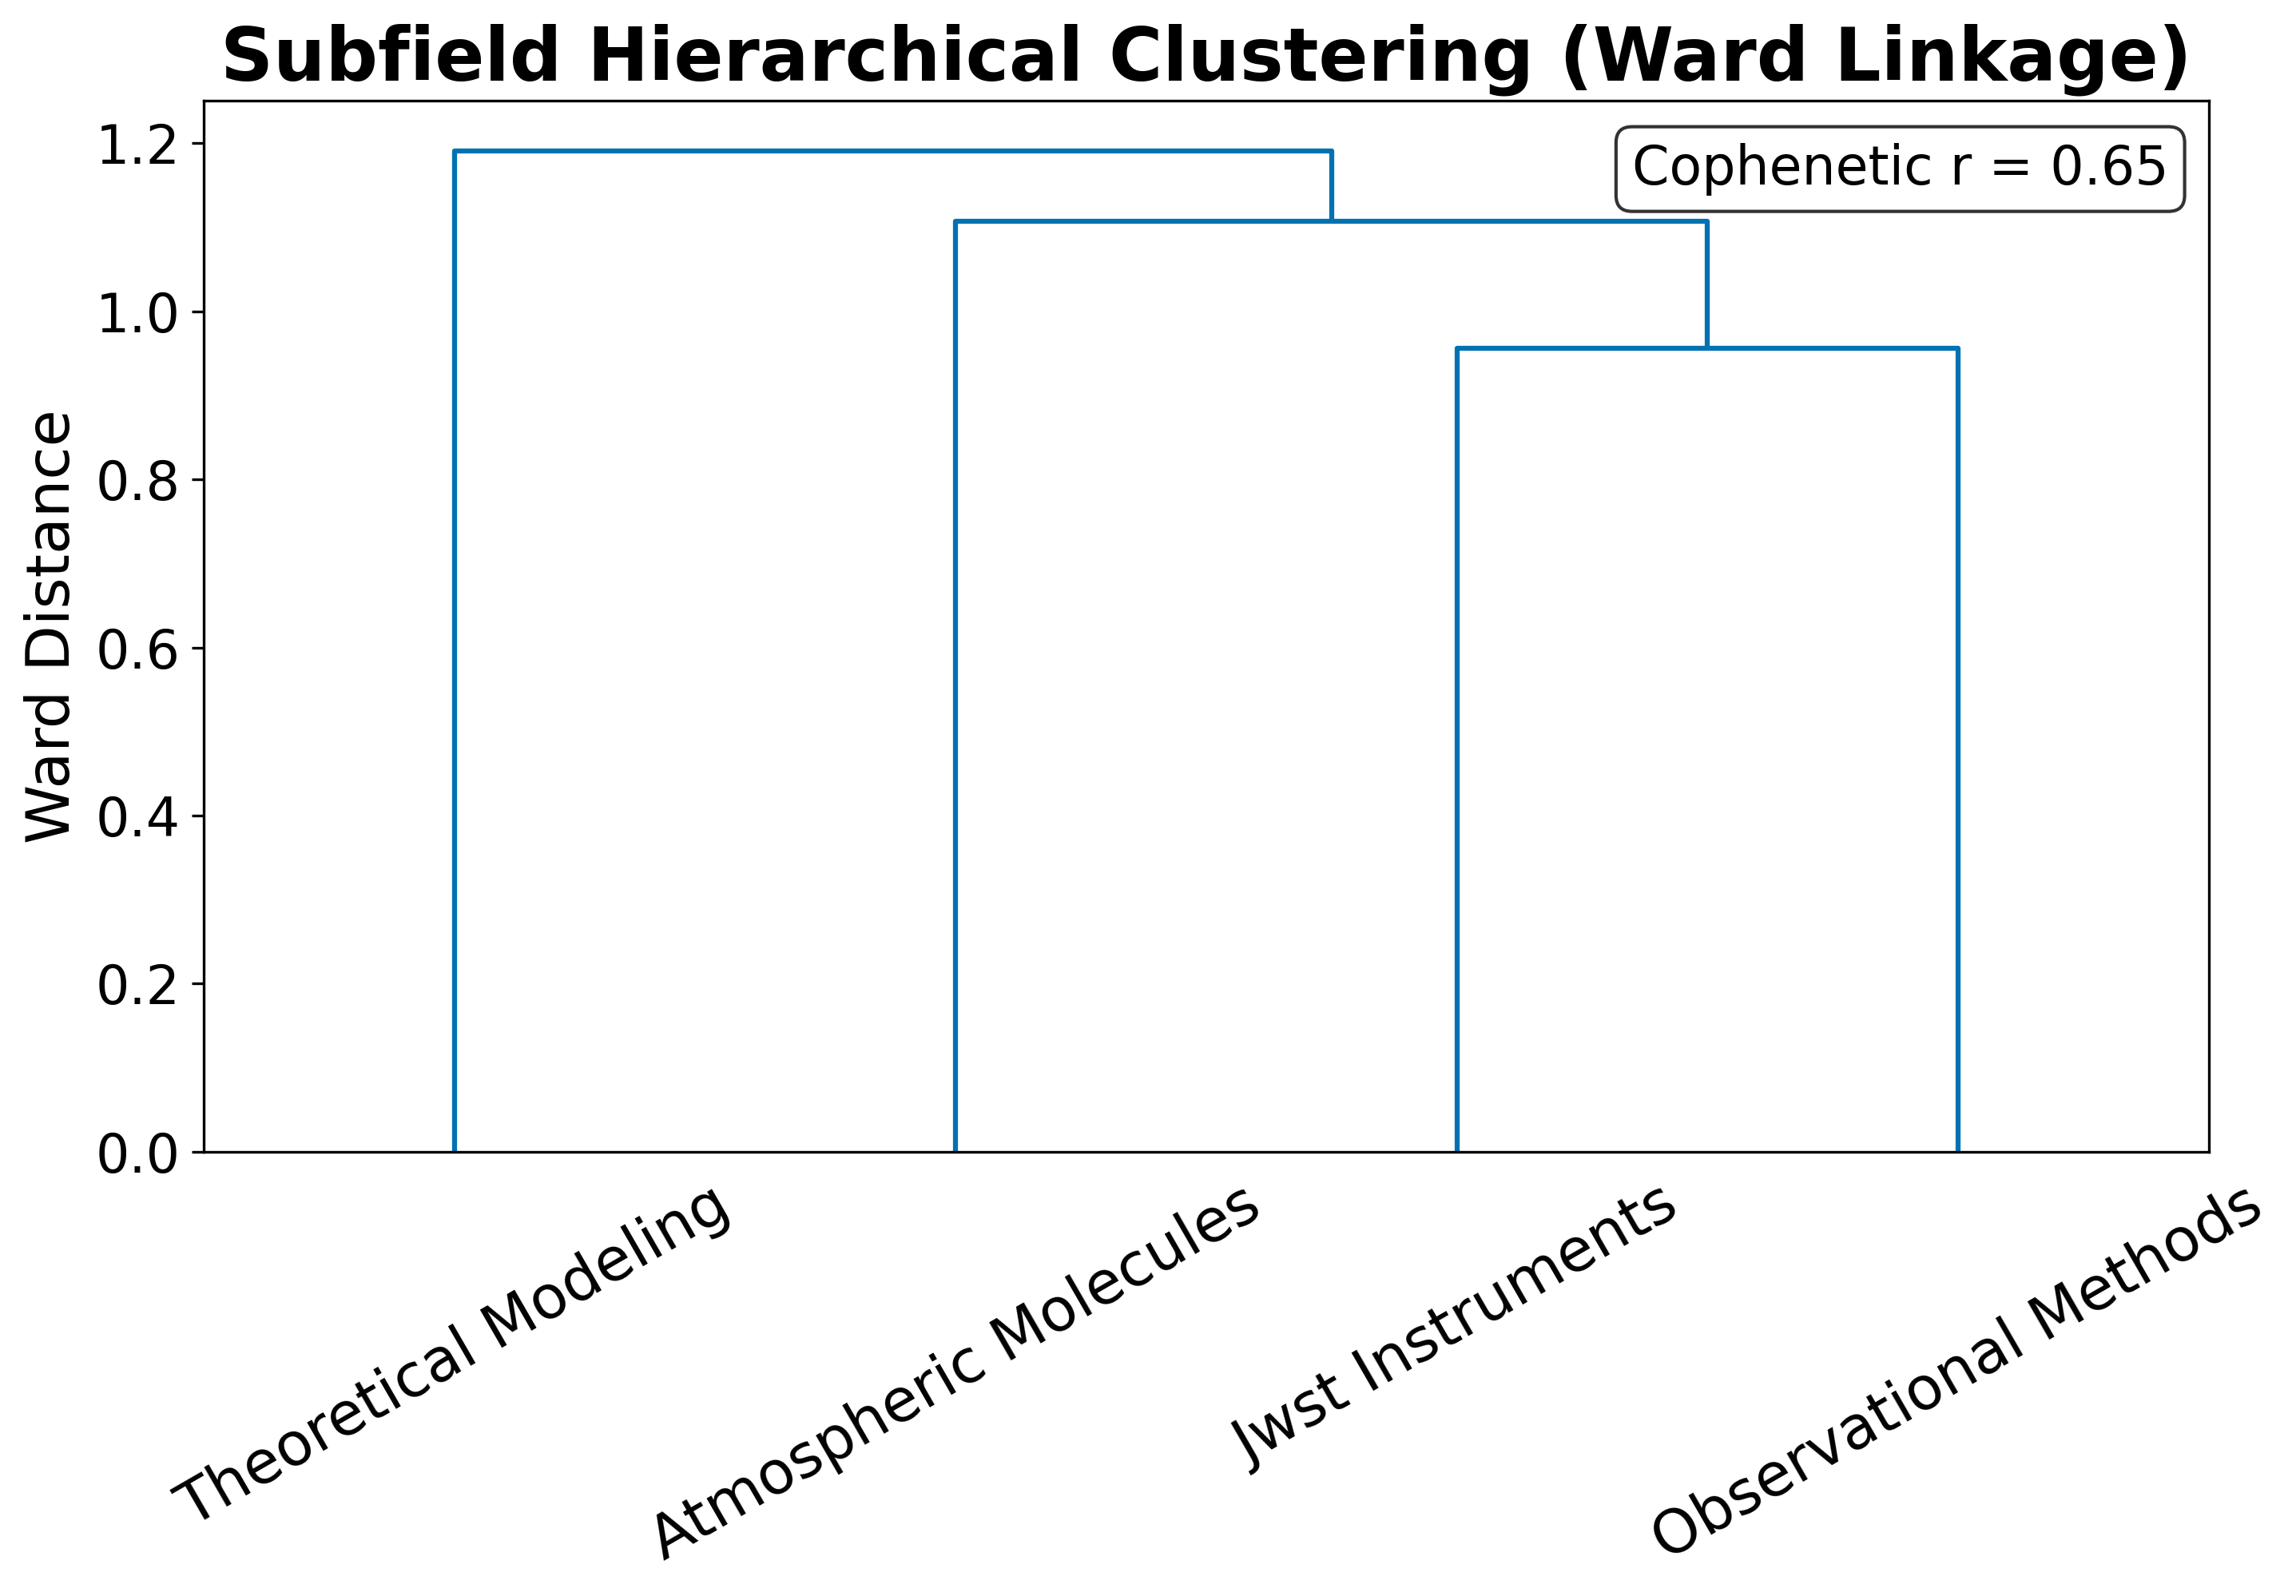
\includegraphics{../figures/dendrogram.png}
\caption{Hierarchical clustering dendrogram of document embeddings. The
tree shows the similarity structure of the corpus: documents that join
low in the tree are semantically similar, while high-level splits
separate the major topical clusters.}\label{fig:dendrogram}
\end{figure}

\subsection{Term Analysis}\label{term-analysis}

The TF-IDF term heatmap reveals which terms discriminate between
subfields: terms with high between-subfield variance (rather than high
global mean) are selected for display.

\begin{figure}
\centering
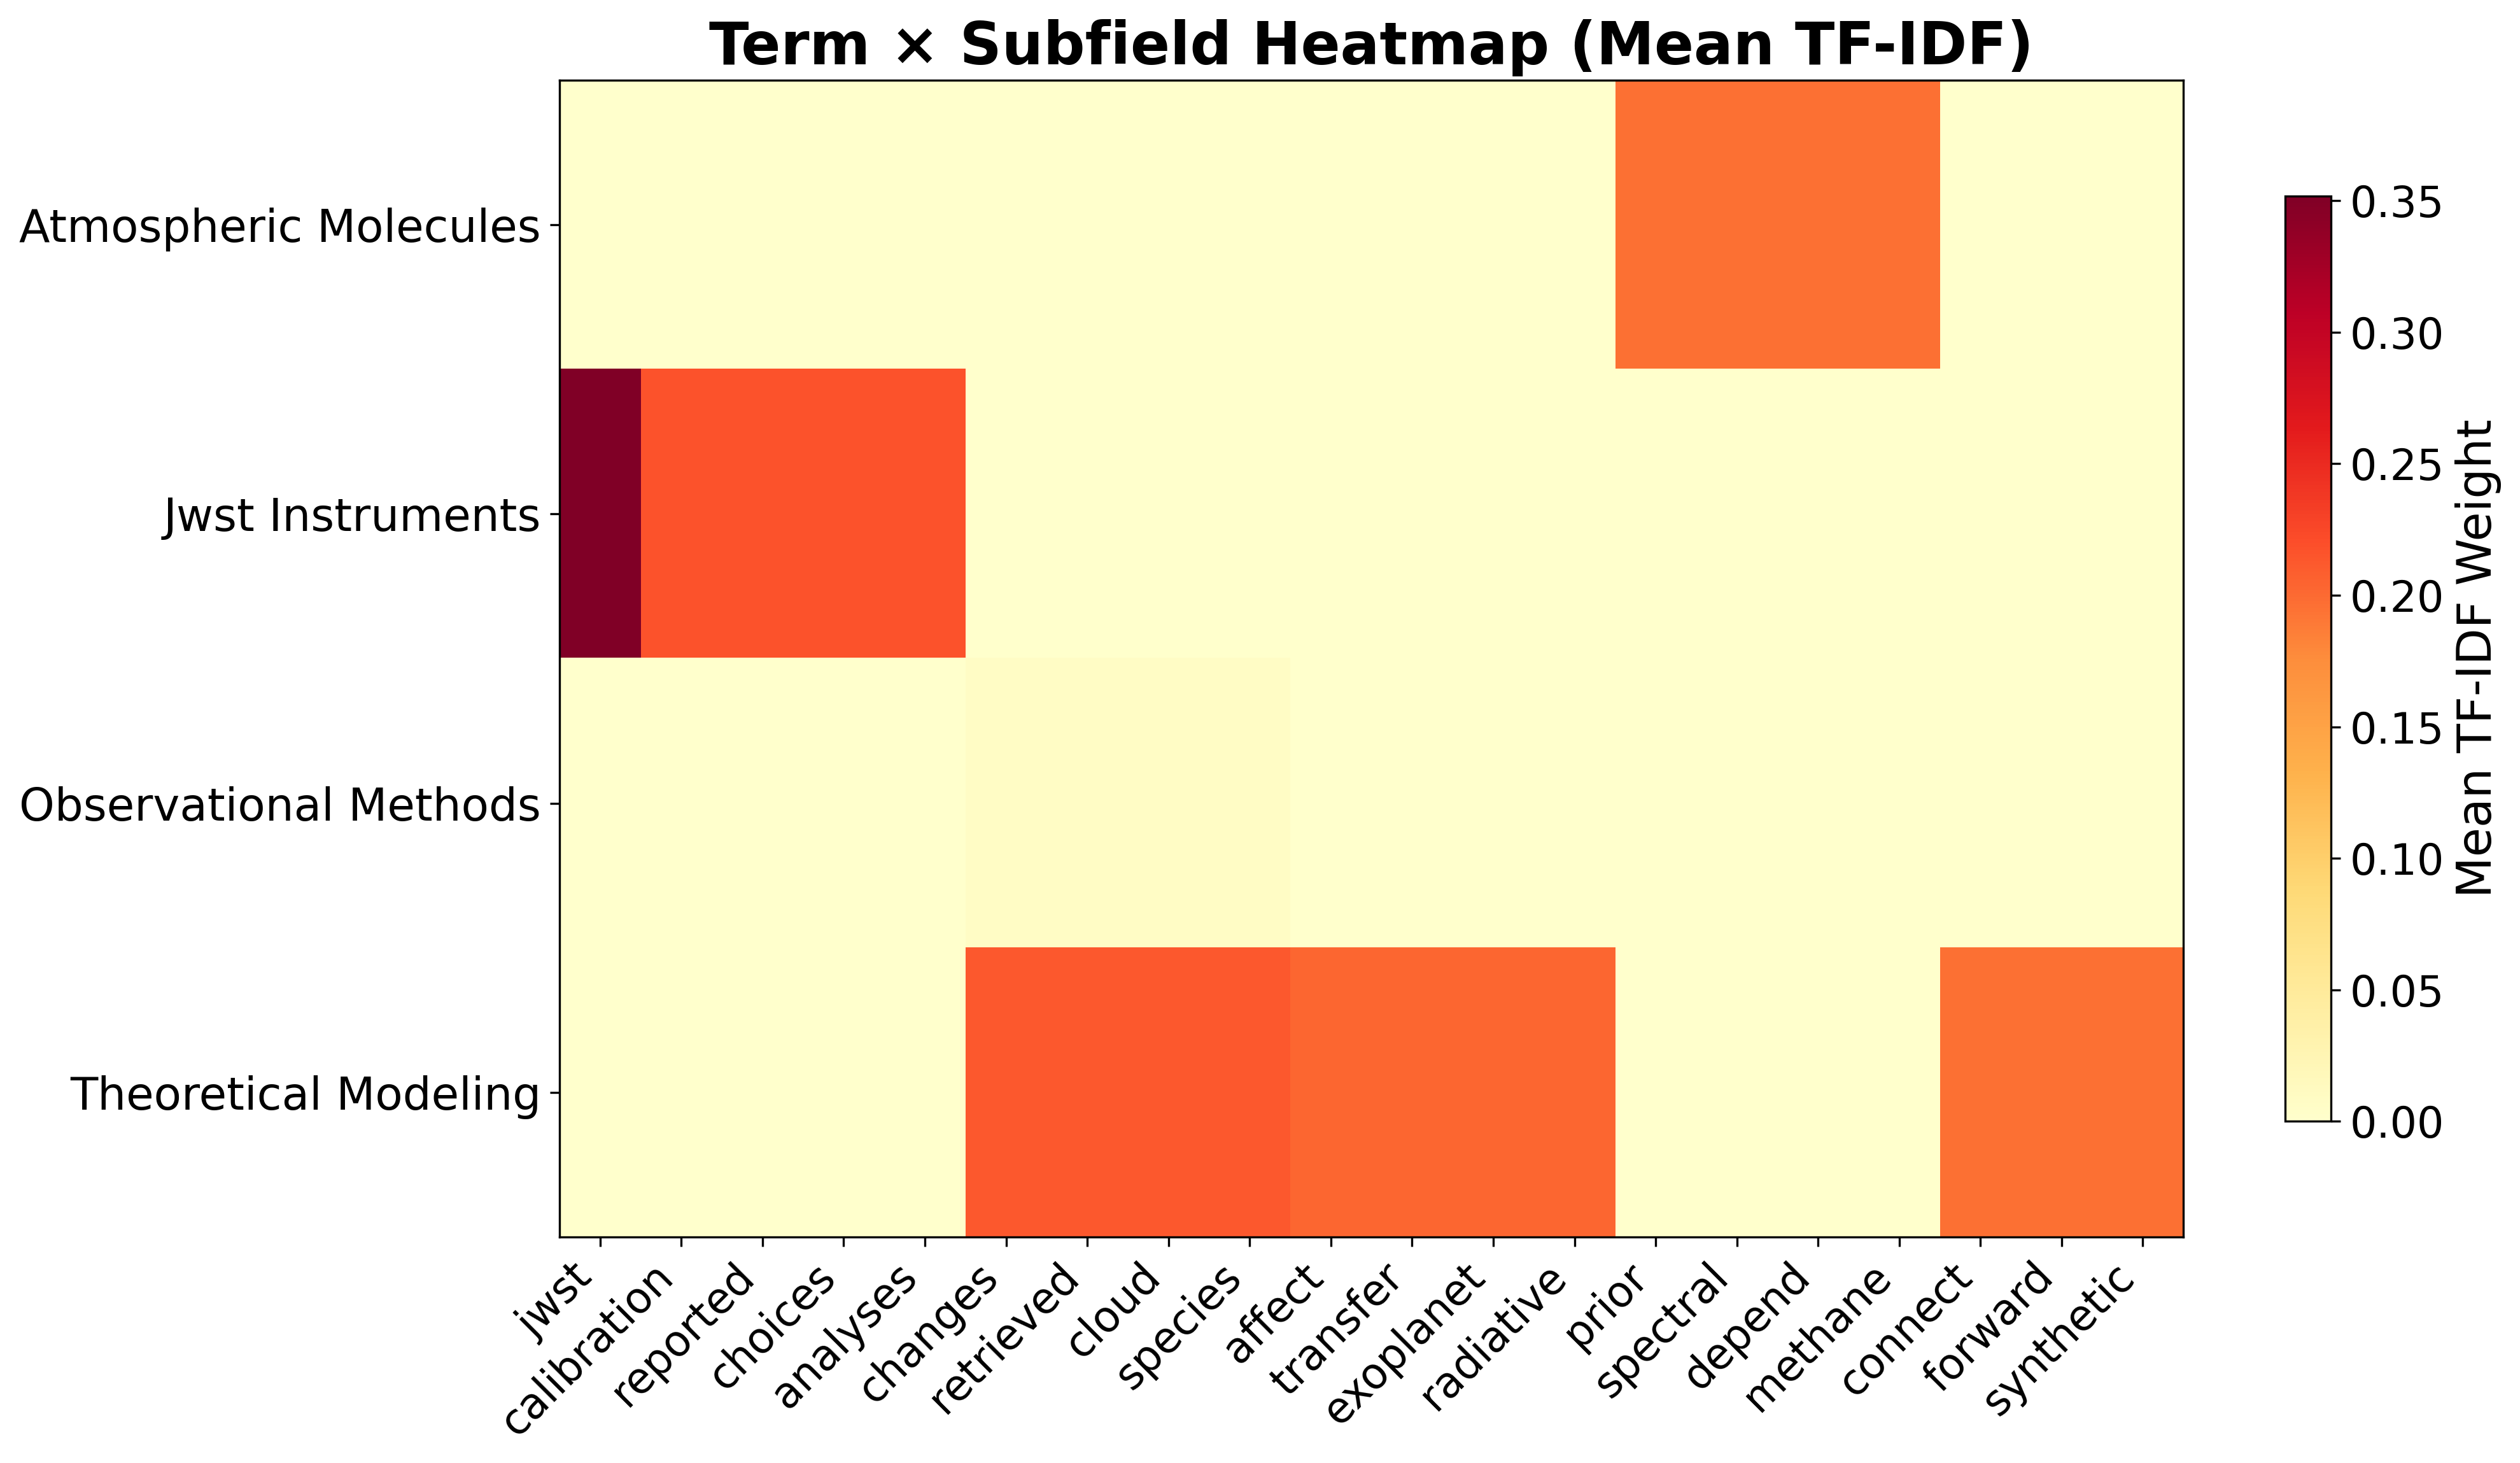
\includegraphics{../figures/term_heatmap.png}
\caption{Term heatmap for \{\{SEARCH\_TERM\_TITLE\}\}. Each cell shows
the mean TF-IDF weight of a term within a subfield. Terms are selected
by between-subfield variance to highlight discriminative vocabulary
rather than globally frequent terms.}\label{fig:term_heatmap}
\end{figure}

\newpage

\subsection{Named Entity Analysis}\label{named-entity-analysis}

Named entity extraction over the \{\{ABSTRACT\_COUNT\}\} abstracts
identified \{\{NUM\_ENTITIES\}\} unique entities. The most frequent
entities reflect the retained corpus and the configured extraction
rules; source coverage and fixture status determine how they may be
interpreted.

\textbf{Table 4. Top named entities in abstracts.}

\{\{TOP\_ENTITIES\_TABLE\}\}

\begin{figure}
\centering
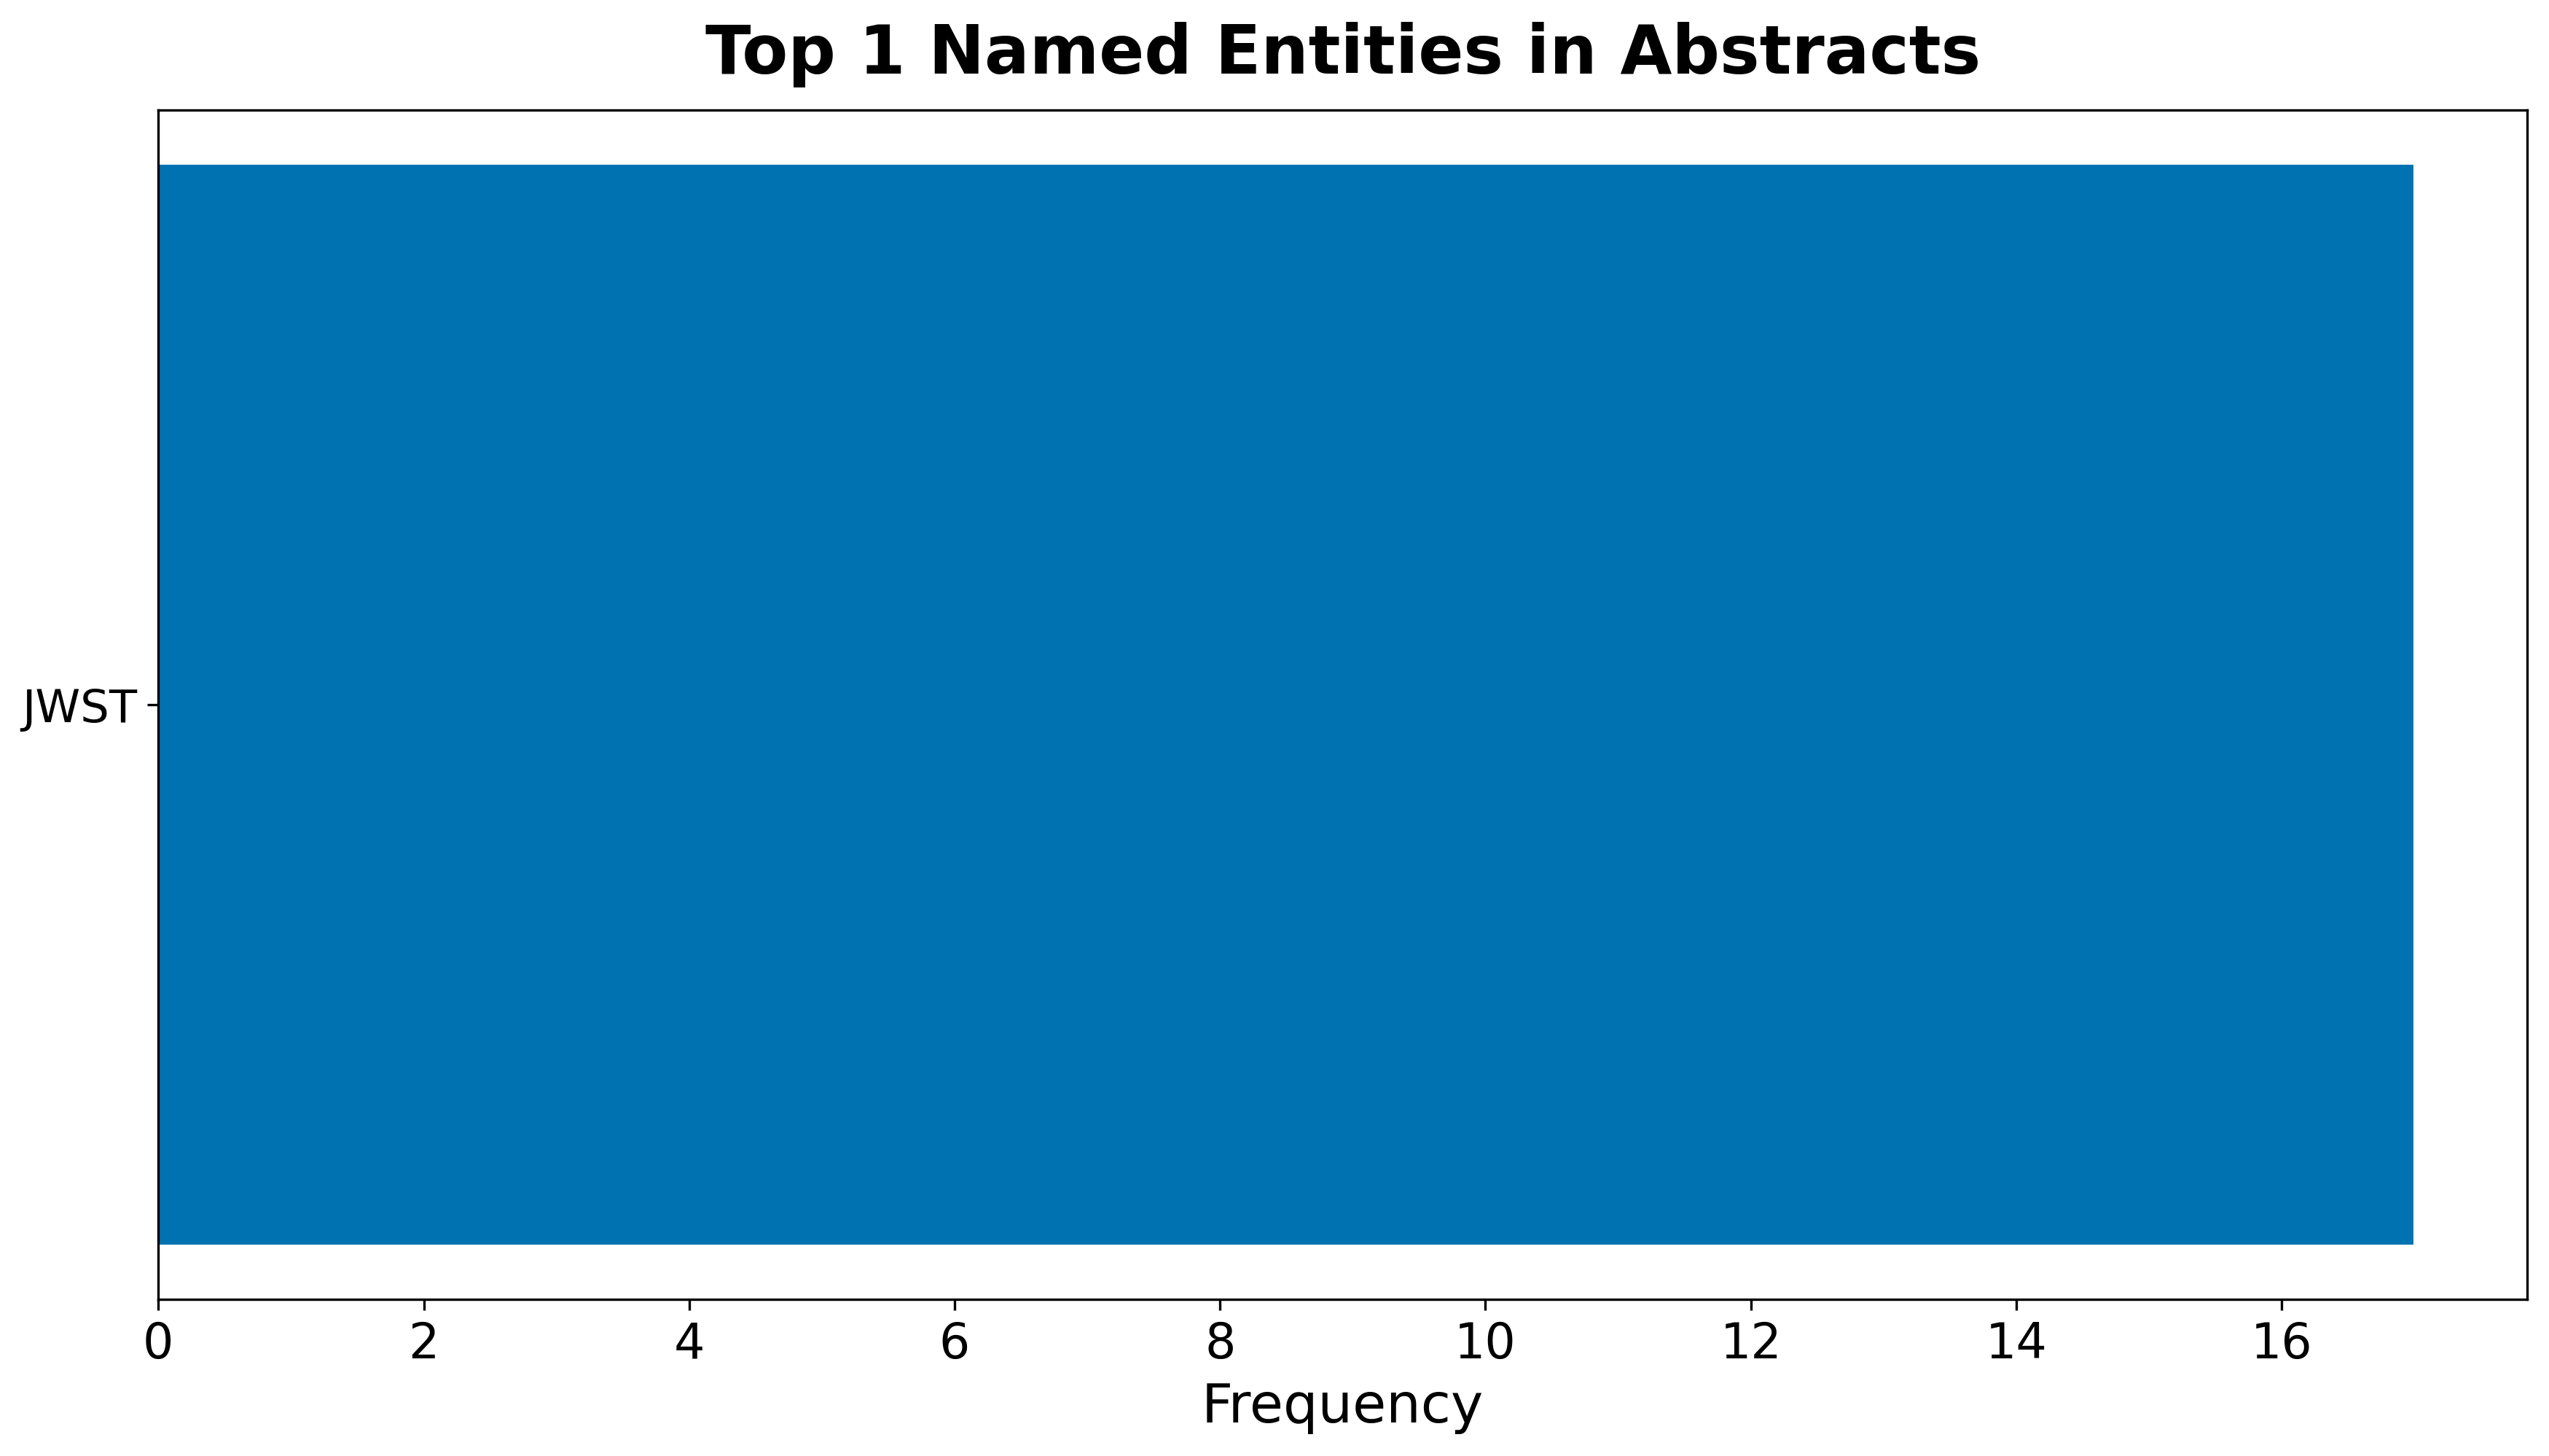
\includegraphics{../figures/entity_bar_chart.png}
\caption{Top named entities for \{\{SEARCH\_TERM\_TITLE\}\}. The
horizontal bar chart shows the 20 most frequently extracted entities
from abstracts, revealing recurring objects, instruments, methods, and
concepts in the retained corpus.}\label{fig:entity_bar_chart}
\end{figure}

\clearpage

\textbf{Table 5. Top keyphrases by TF-IDF score.}

\{\{TOP\_KEYPHRASES\_TABLE\}\}

\subsection{Embedding Similarity and
Clustering}\label{embedding-similarity-and-clustering}

The TF-IDF/SVD embeddings place every document in a 50-dimensional
vector space. K-means clustering with \(k = {{NUM_EMBEDDING_CLUSTERS}}\)
clusters partitions the corpus into topically coherent groups. The top
similar document pairs, ranked by cosine similarity, reveal the most
closely related works in the corpus.

\textbf{Table 6. Top 10 most similar document pairs.}

\{\{TOP\_SIMILAR\_PAIRS\_TABLE\}\}

\begin{figure}
\centering
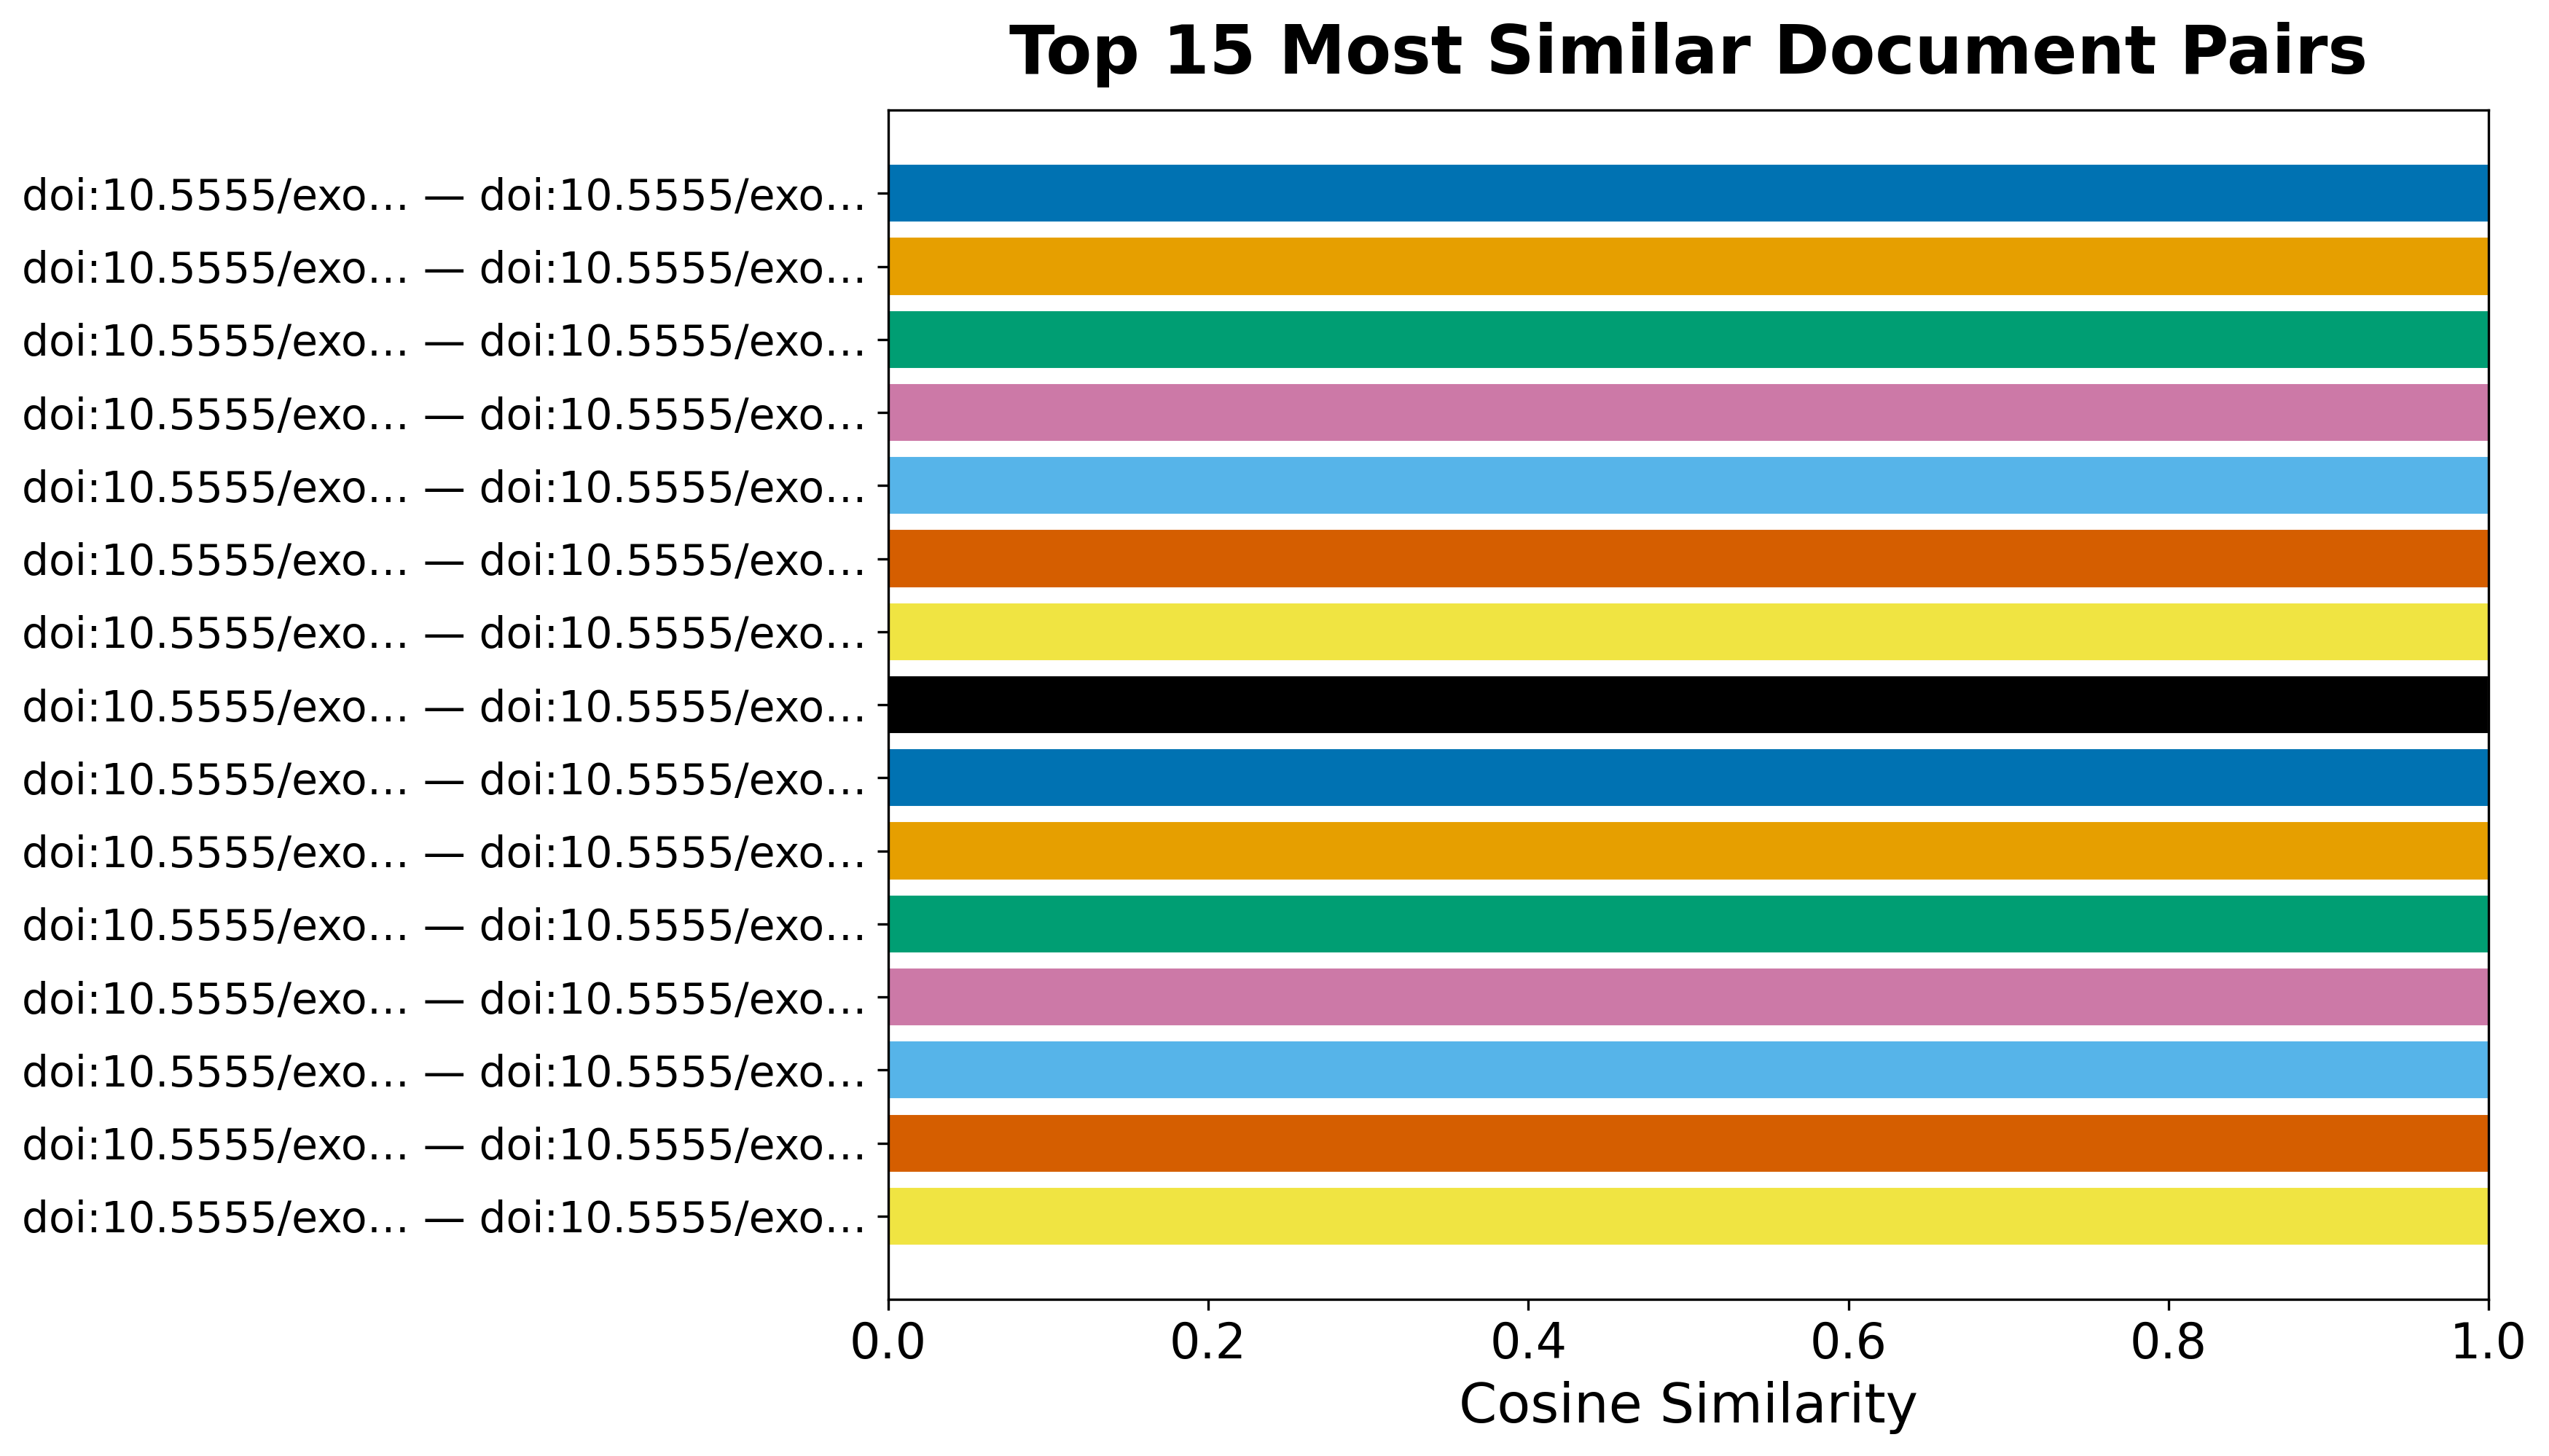
\includegraphics{../figures/similarity_heatmap.png}
\caption{Document similarity for \{\{SEARCH\_TERM\_TITLE\}\}. The
horizontal bar chart shows the 15 most similar document pairs ranked by
cosine similarity of their TF-IDF/SVD embeddings. High-similarity pairs
share topical and lexical content.}\label{fig:similarity_heatmap}
\end{figure}

\begin{figure}
\centering
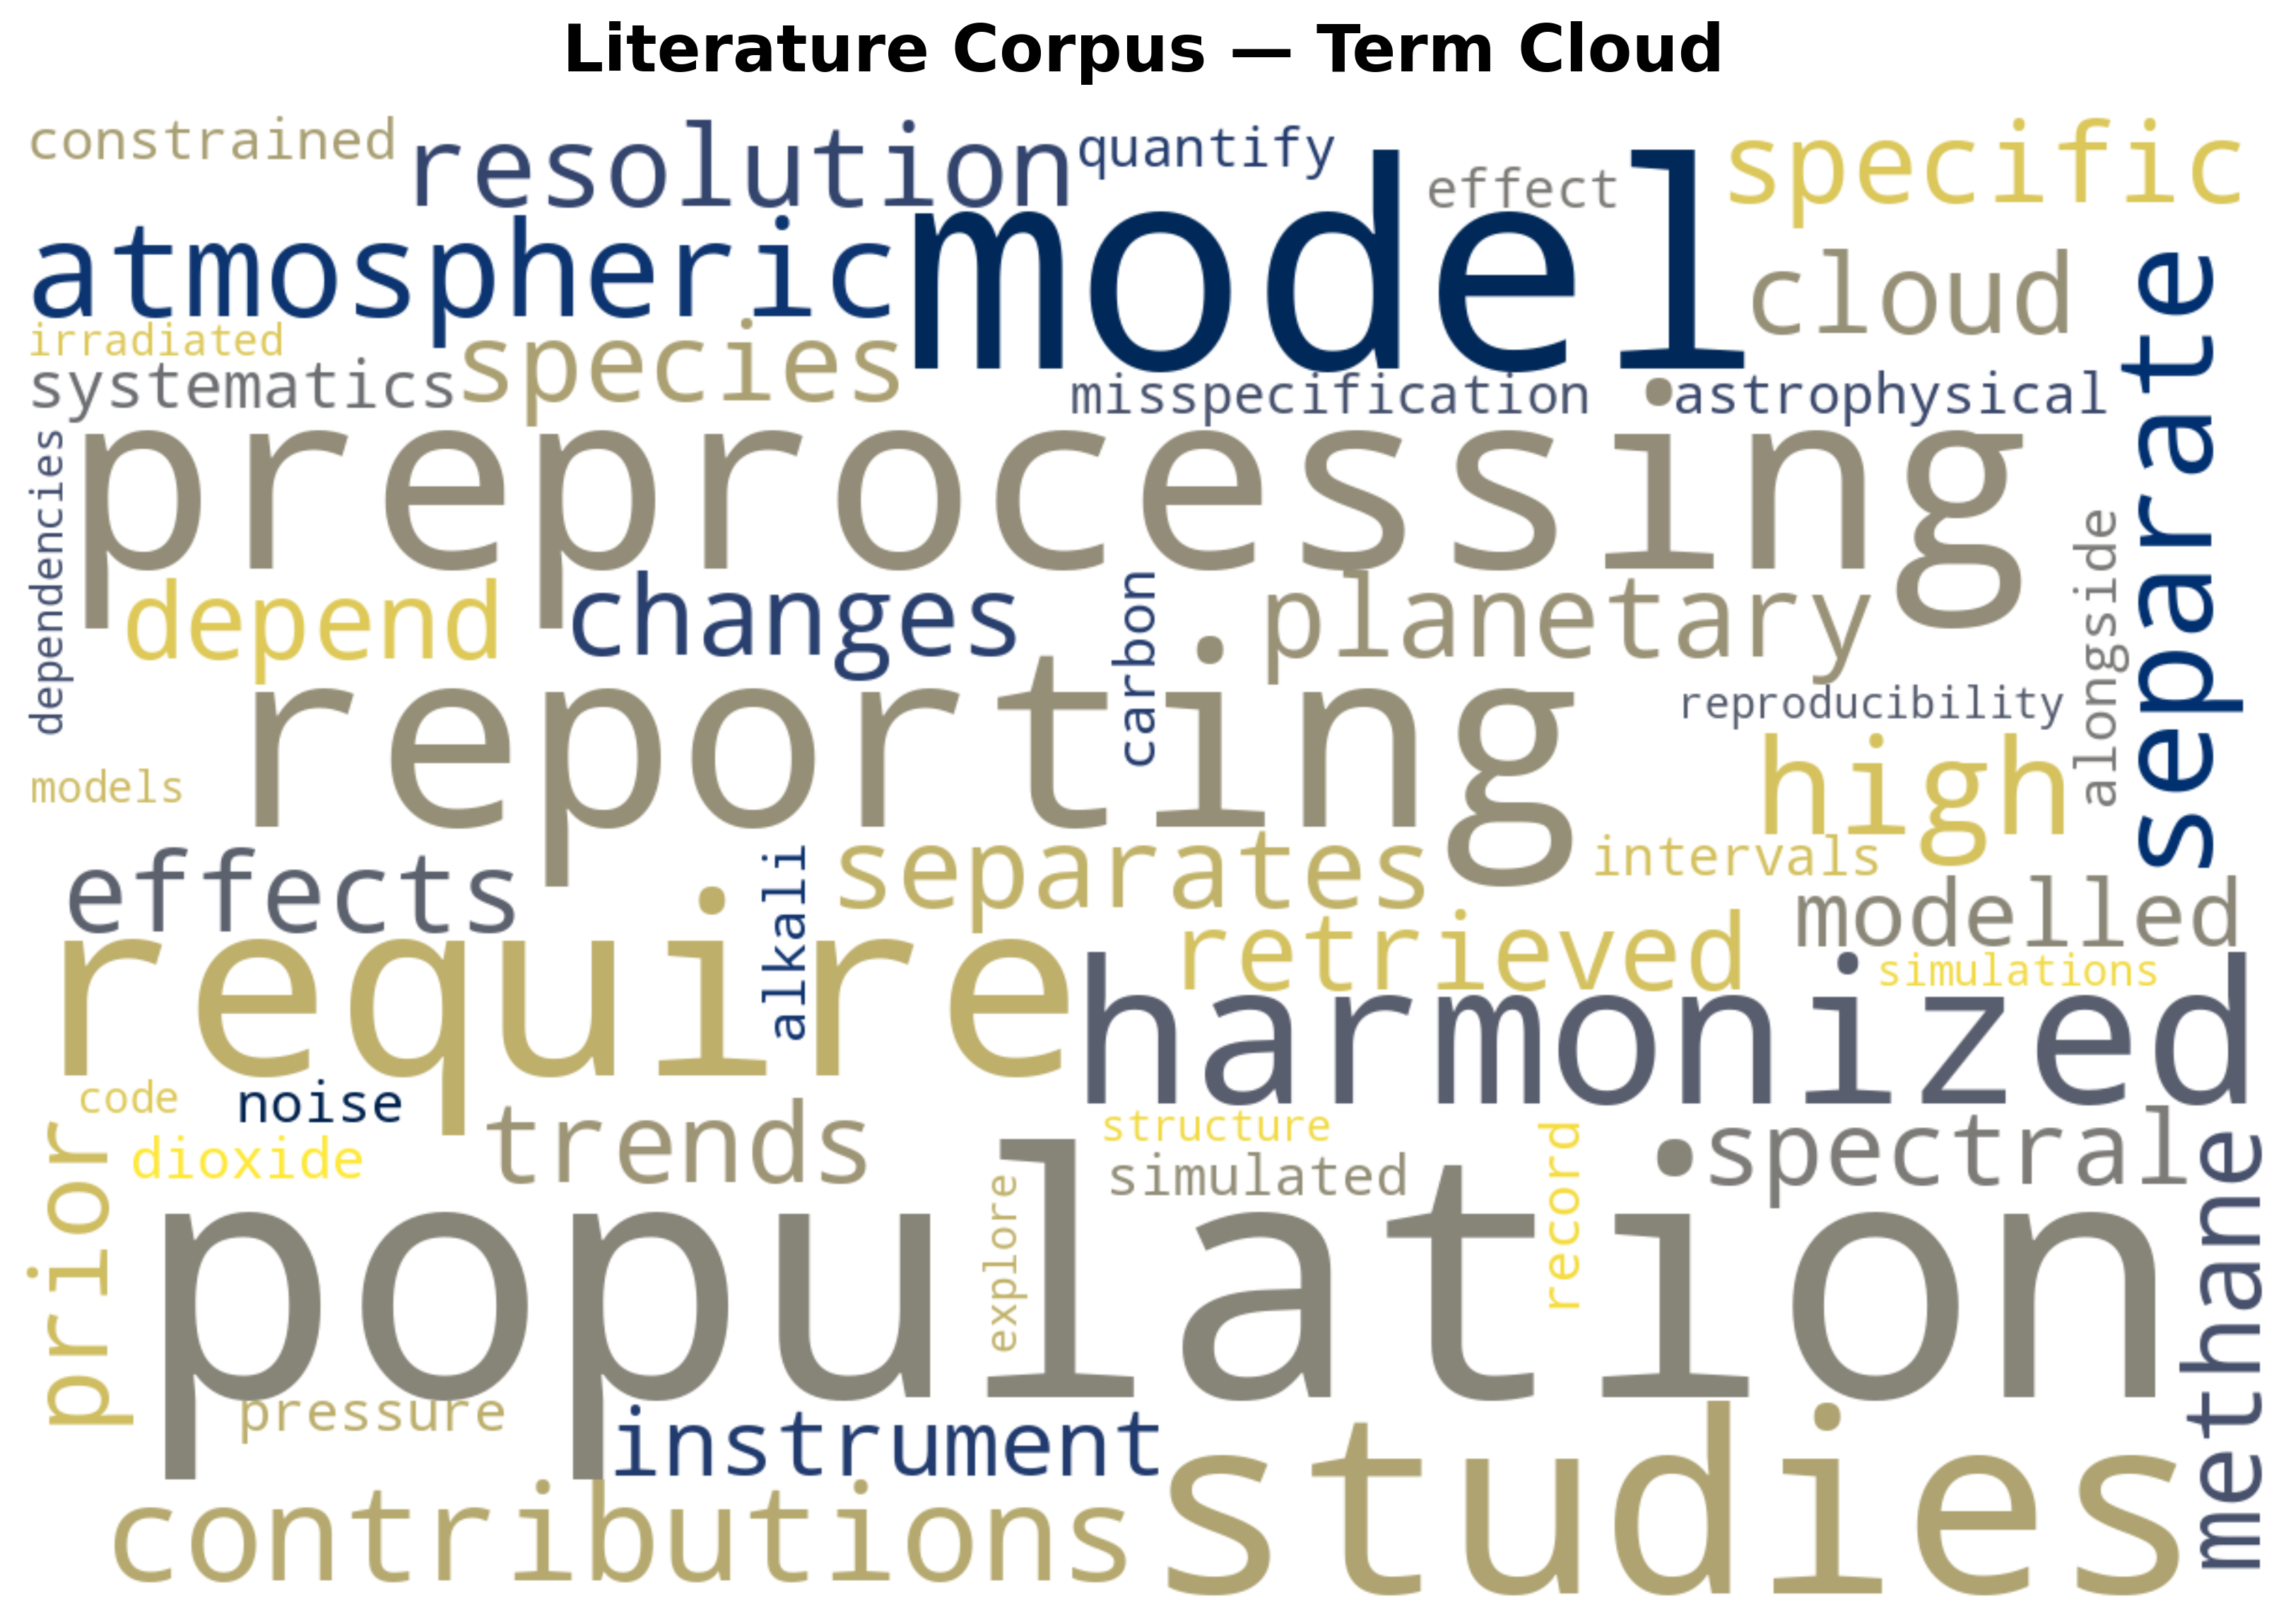
\includegraphics{../figures/word_cloud.png}
\caption{Term cloud for \{\{SEARCH\_TERM\_TITLE\}\}. Term sizes are
proportional to their TF-IDF weights across the corpus, providing a
visual summary of the dominant vocabulary.}\label{fig:word_cloud}
\end{figure}

\begin{figure}
\centering
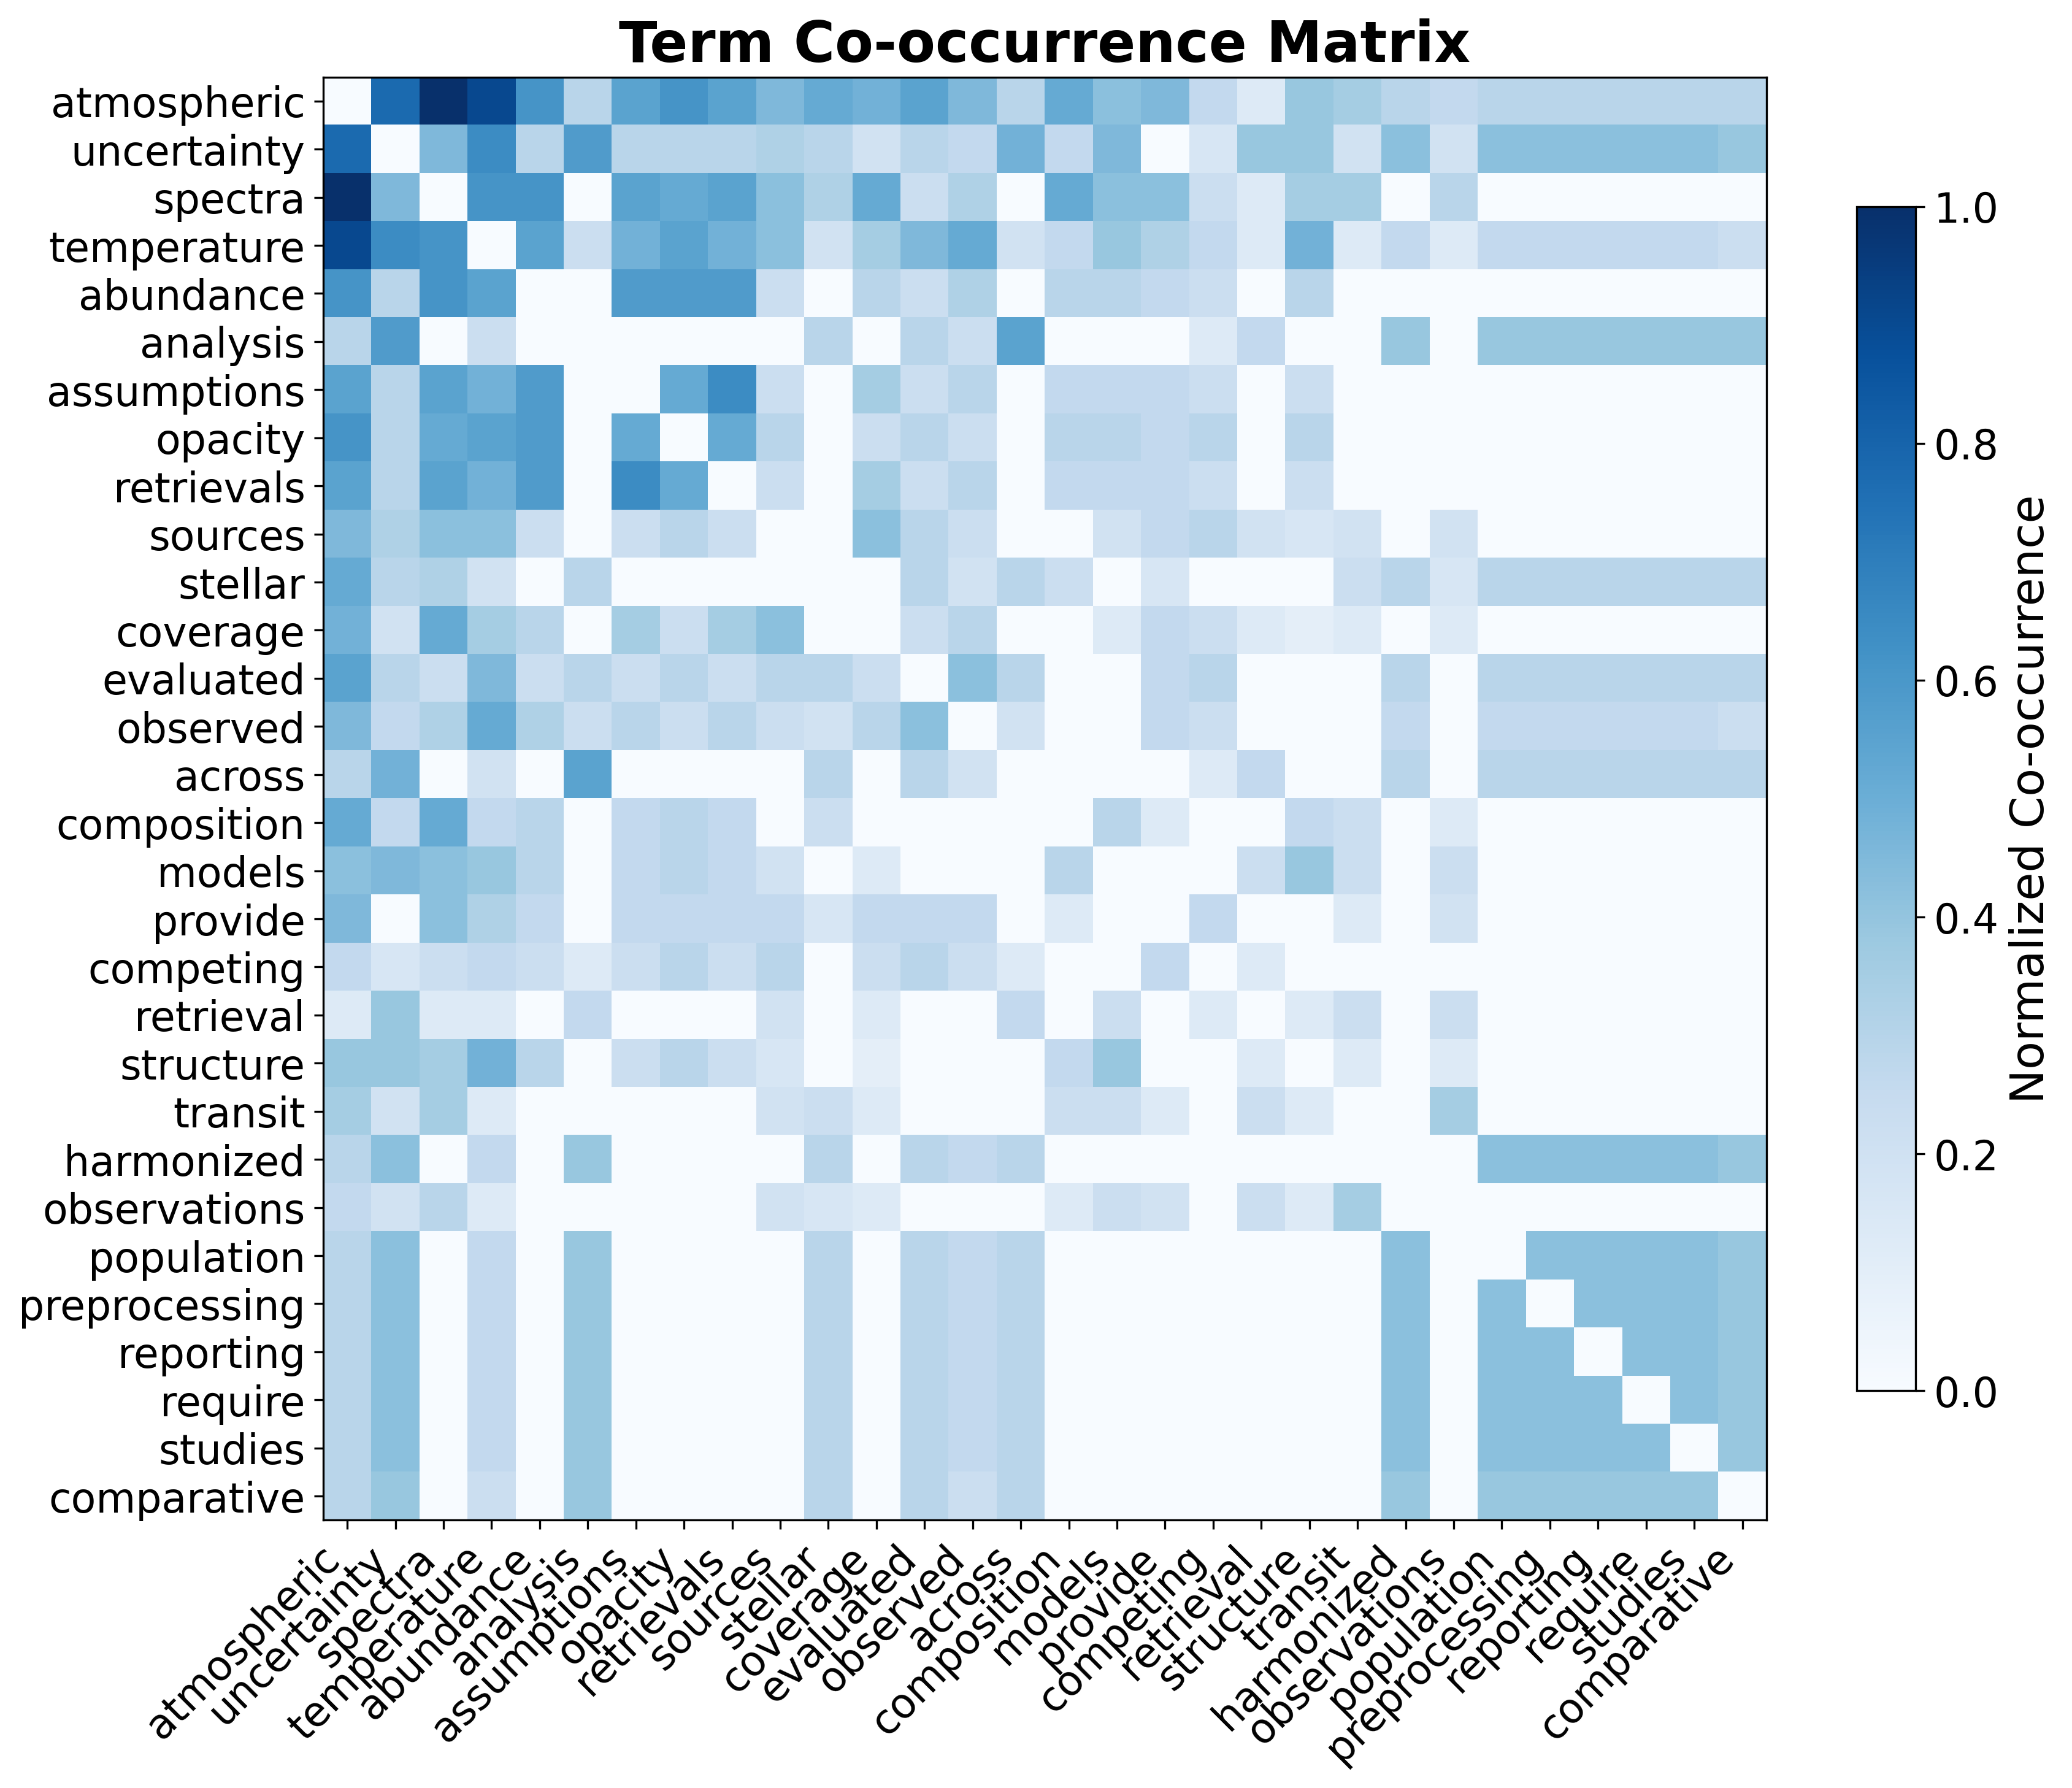
\includegraphics{../figures/cooccurrence_matrix.png}
\caption{Term co-occurrence matrix for \{\{SEARCH\_TERM\_TITLE\}\}. Each
cell shows the normalized co-occurrence frequency of two terms within
the same document, revealing which concepts tend to appear together in
the literature.}\label{fig:cooccurrence_matrix}
\end{figure}

These embeddings support semantic retrieval over the corpus and the
visual map of the literature's topical geography.

\newpage

\section{Results: Citation Network}\label{results-citation-network}

\subsection{RQ4: Citation Geometry}\label{rq4-citation-geometry}

Resolving each record's references against the corpus yields an
intra-corpus citation graph (built and analyzed with NetworkX
\citep{hagberg2008exploring}) of \{\{CITATION\_NODES\}\} nodes and
\{\{CITATION\_EDGES\}\} edges across \{\{CITATION\_COMPONENTS\}\}
connected components, with a graph density of
\{\{CITATION\_DENSITY\_PCT\}\}\% and a mean in-degree of
\{\{MEAN\_IN\_DEGREE\}\}. Of \{\{CITATION\_TOTAL\_REFS\}\} total
outgoing references, \{\{CITATION\_RESOLUTION\_PCT\}\}\% resolve to
another record inside the corpus. This resolution rate describes how
self-contained the retrieved slice is; it is not an estimate of the
underlying citation density of any individual work.

The citation network has \{\{CITATION\_COMMUNITIES\}\} communities
(detected by modularity optimization), a maximum in-degree of
\{\{CITATION\_MAX\_IN\_DEGREE\}\} (the most-cited paper within the
corpus), and a maximum out-degree of \{\{CITATION\_MAX\_OUT\_DEGREE\}\}
(the paper that cites the most other corpus members).

\subsection{Centrality Analysis}\label{centrality-analysis}

Centrality scores (PageRank \citep{page1999pagerank} and HITS) and
modularity-based community detection \citep{clauset2004finding} are
rounded and ranked with a stable tiebreaker so the reported hub and
authority rankings are byte-reproducible across runs despite the
floating-point non-associativity of the underlying iterative solvers.

\textbf{Table 4. Top 5 papers by PageRank.}

\{\{TOP\_PAGERANK\_TABLE\}\}

\textbf{Table 5. Top 5 authority papers (HITS).}

\{\{TOP\_AUTHORITIES\_TABLE\}\}

\textbf{Table 6. Top 5 hub papers (HITS).}

\{\{TOP\_HUBS\_TABLE\}\}

The highest-ranked paper by PageRank (DOI \{\{TOP\_PAGERANK\_DOI\}\}) is
a central node in the retained citation graph. Its score indicates
relative centrality within this graph, not scientific importance or
causal influence. Hub papers cite many corpus members and may connect
threads of the retrieved literature, but their role should be checked
against their source type and content.

\begin{figure}
\centering
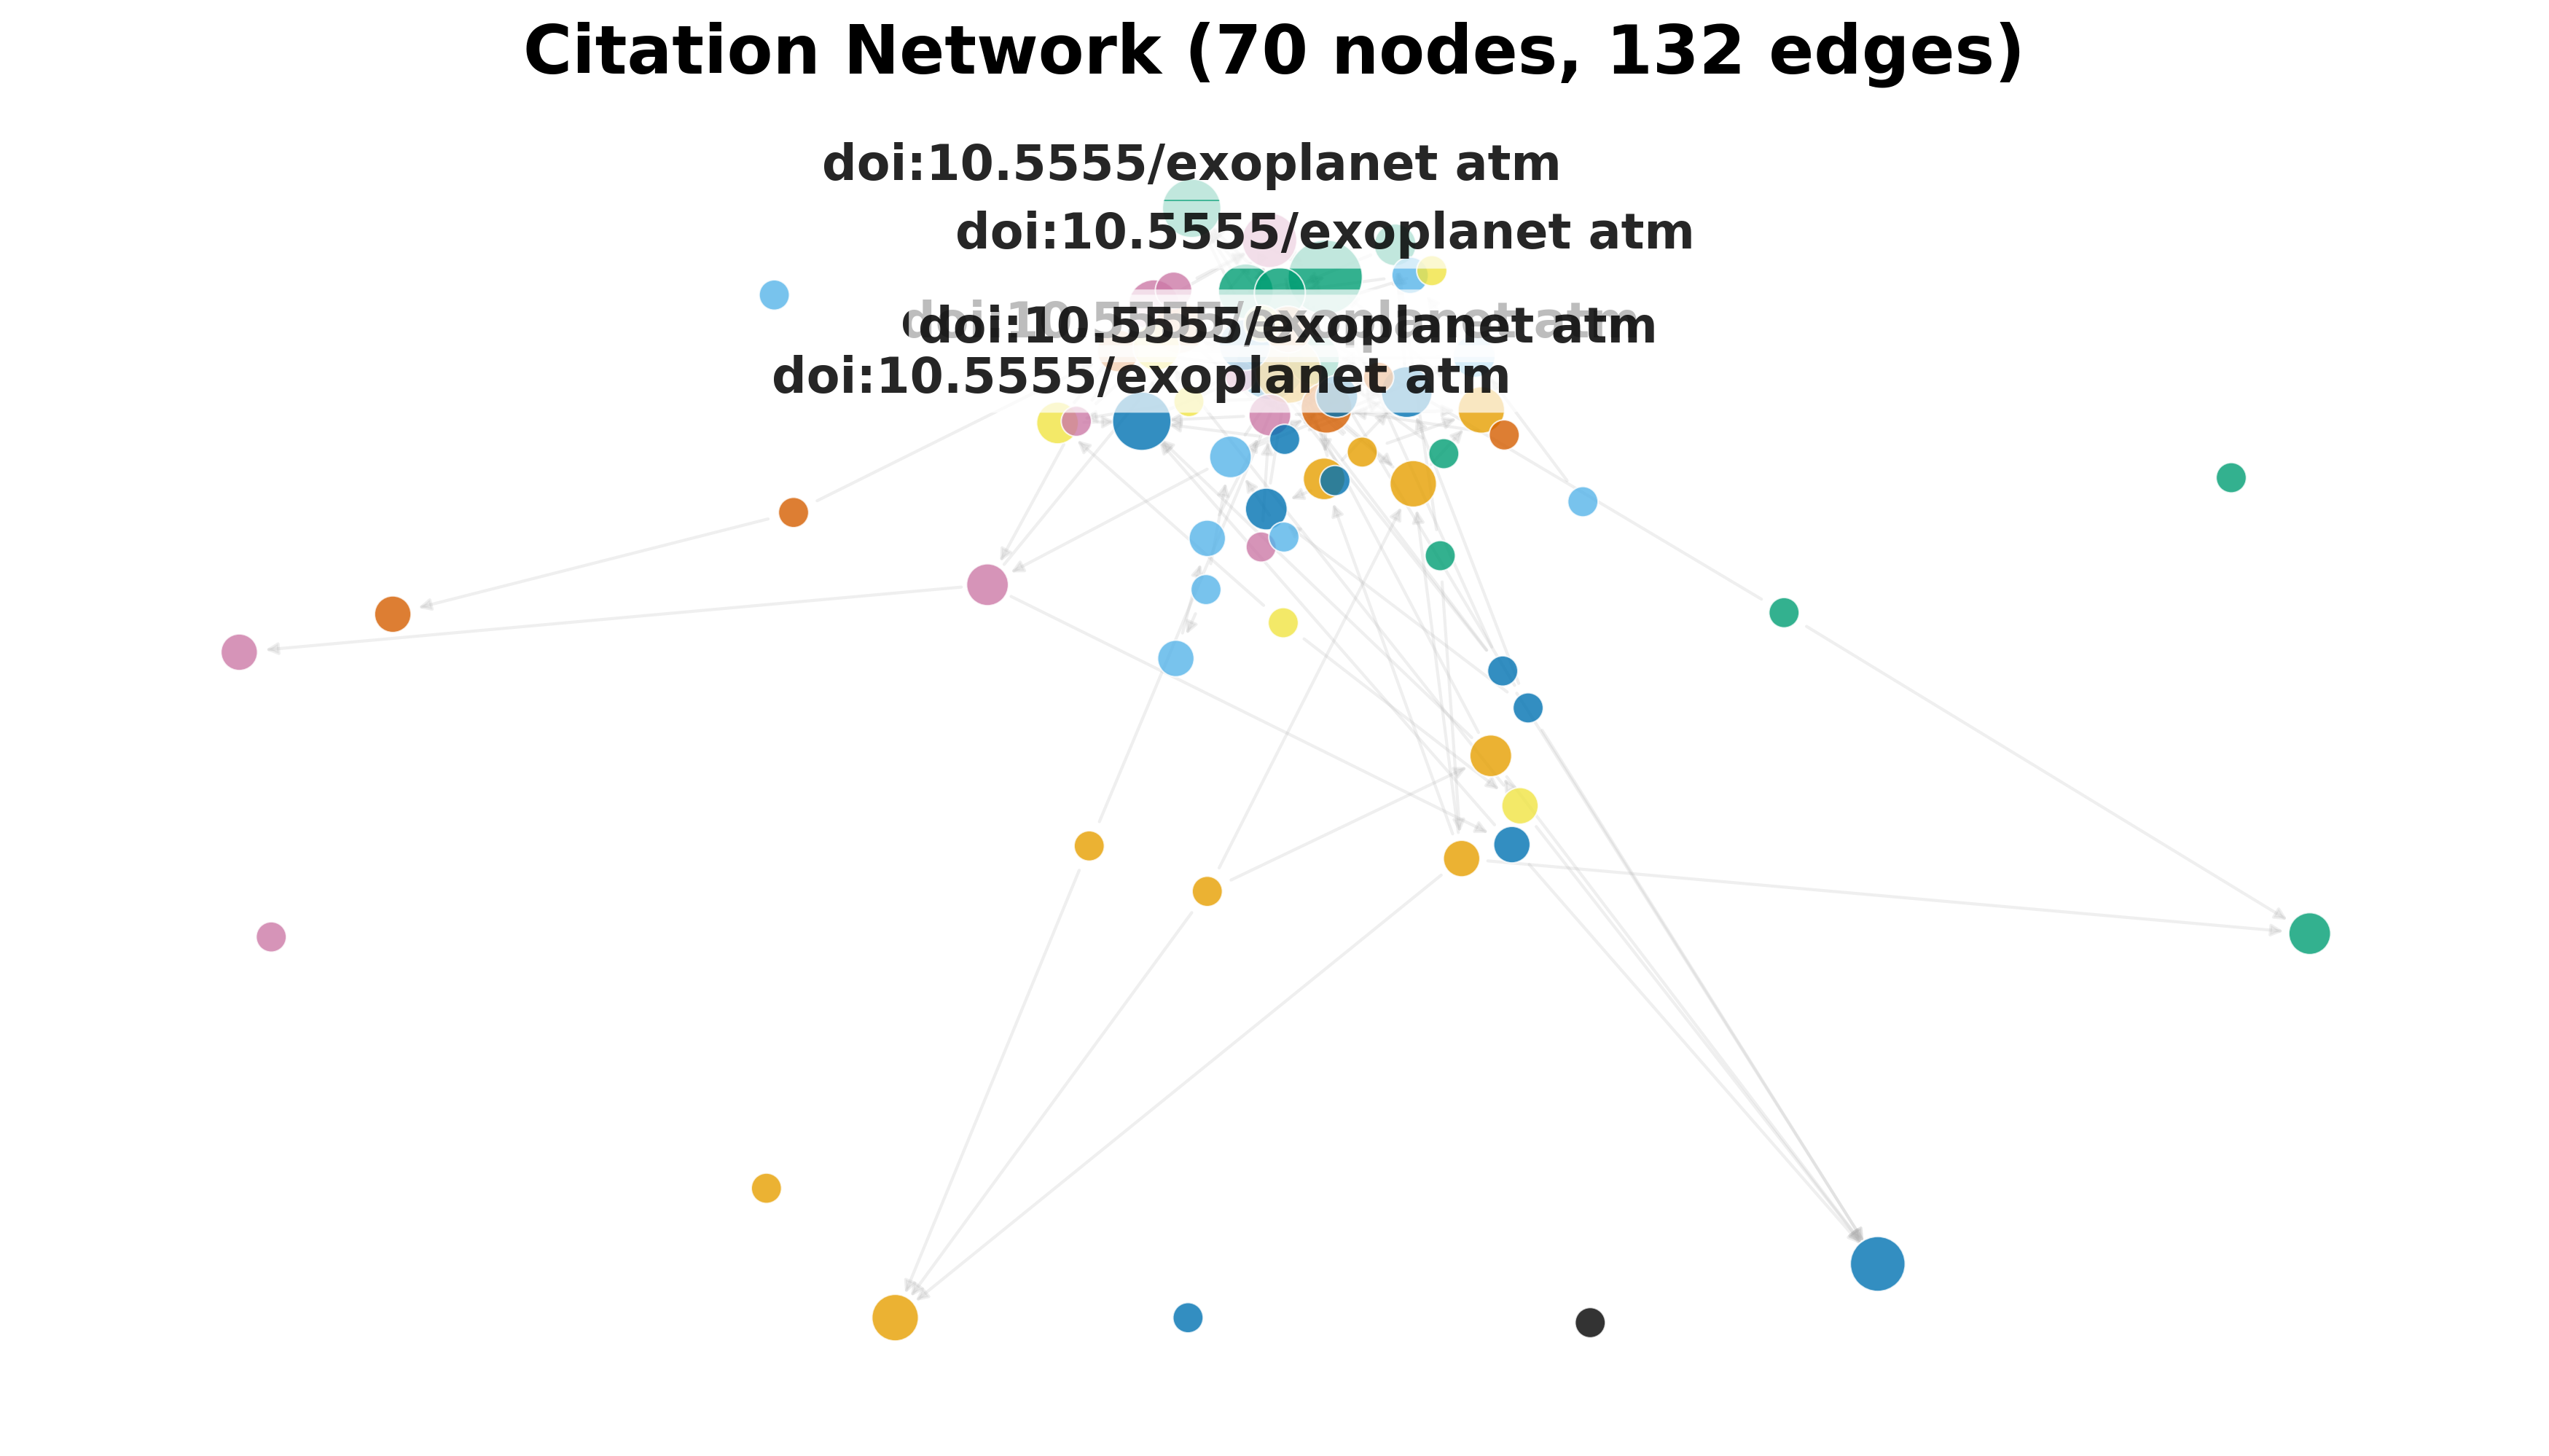
\includegraphics{../figures/citation_network.png}
\caption{Citation network for \{\{SEARCH\_TERM\_TITLE\}\}. Nodes
represent papers; directed edges represent citation links. Node colours
indicate community membership (\{\{CITATION\_COMMUNITIES\}\} communities
detected by modularity optimization). Layout uses a spring-based
algorithm with a fixed seed for
reproducibility.}\label{fig:citation_network}
\end{figure}

\begin{figure}
\centering
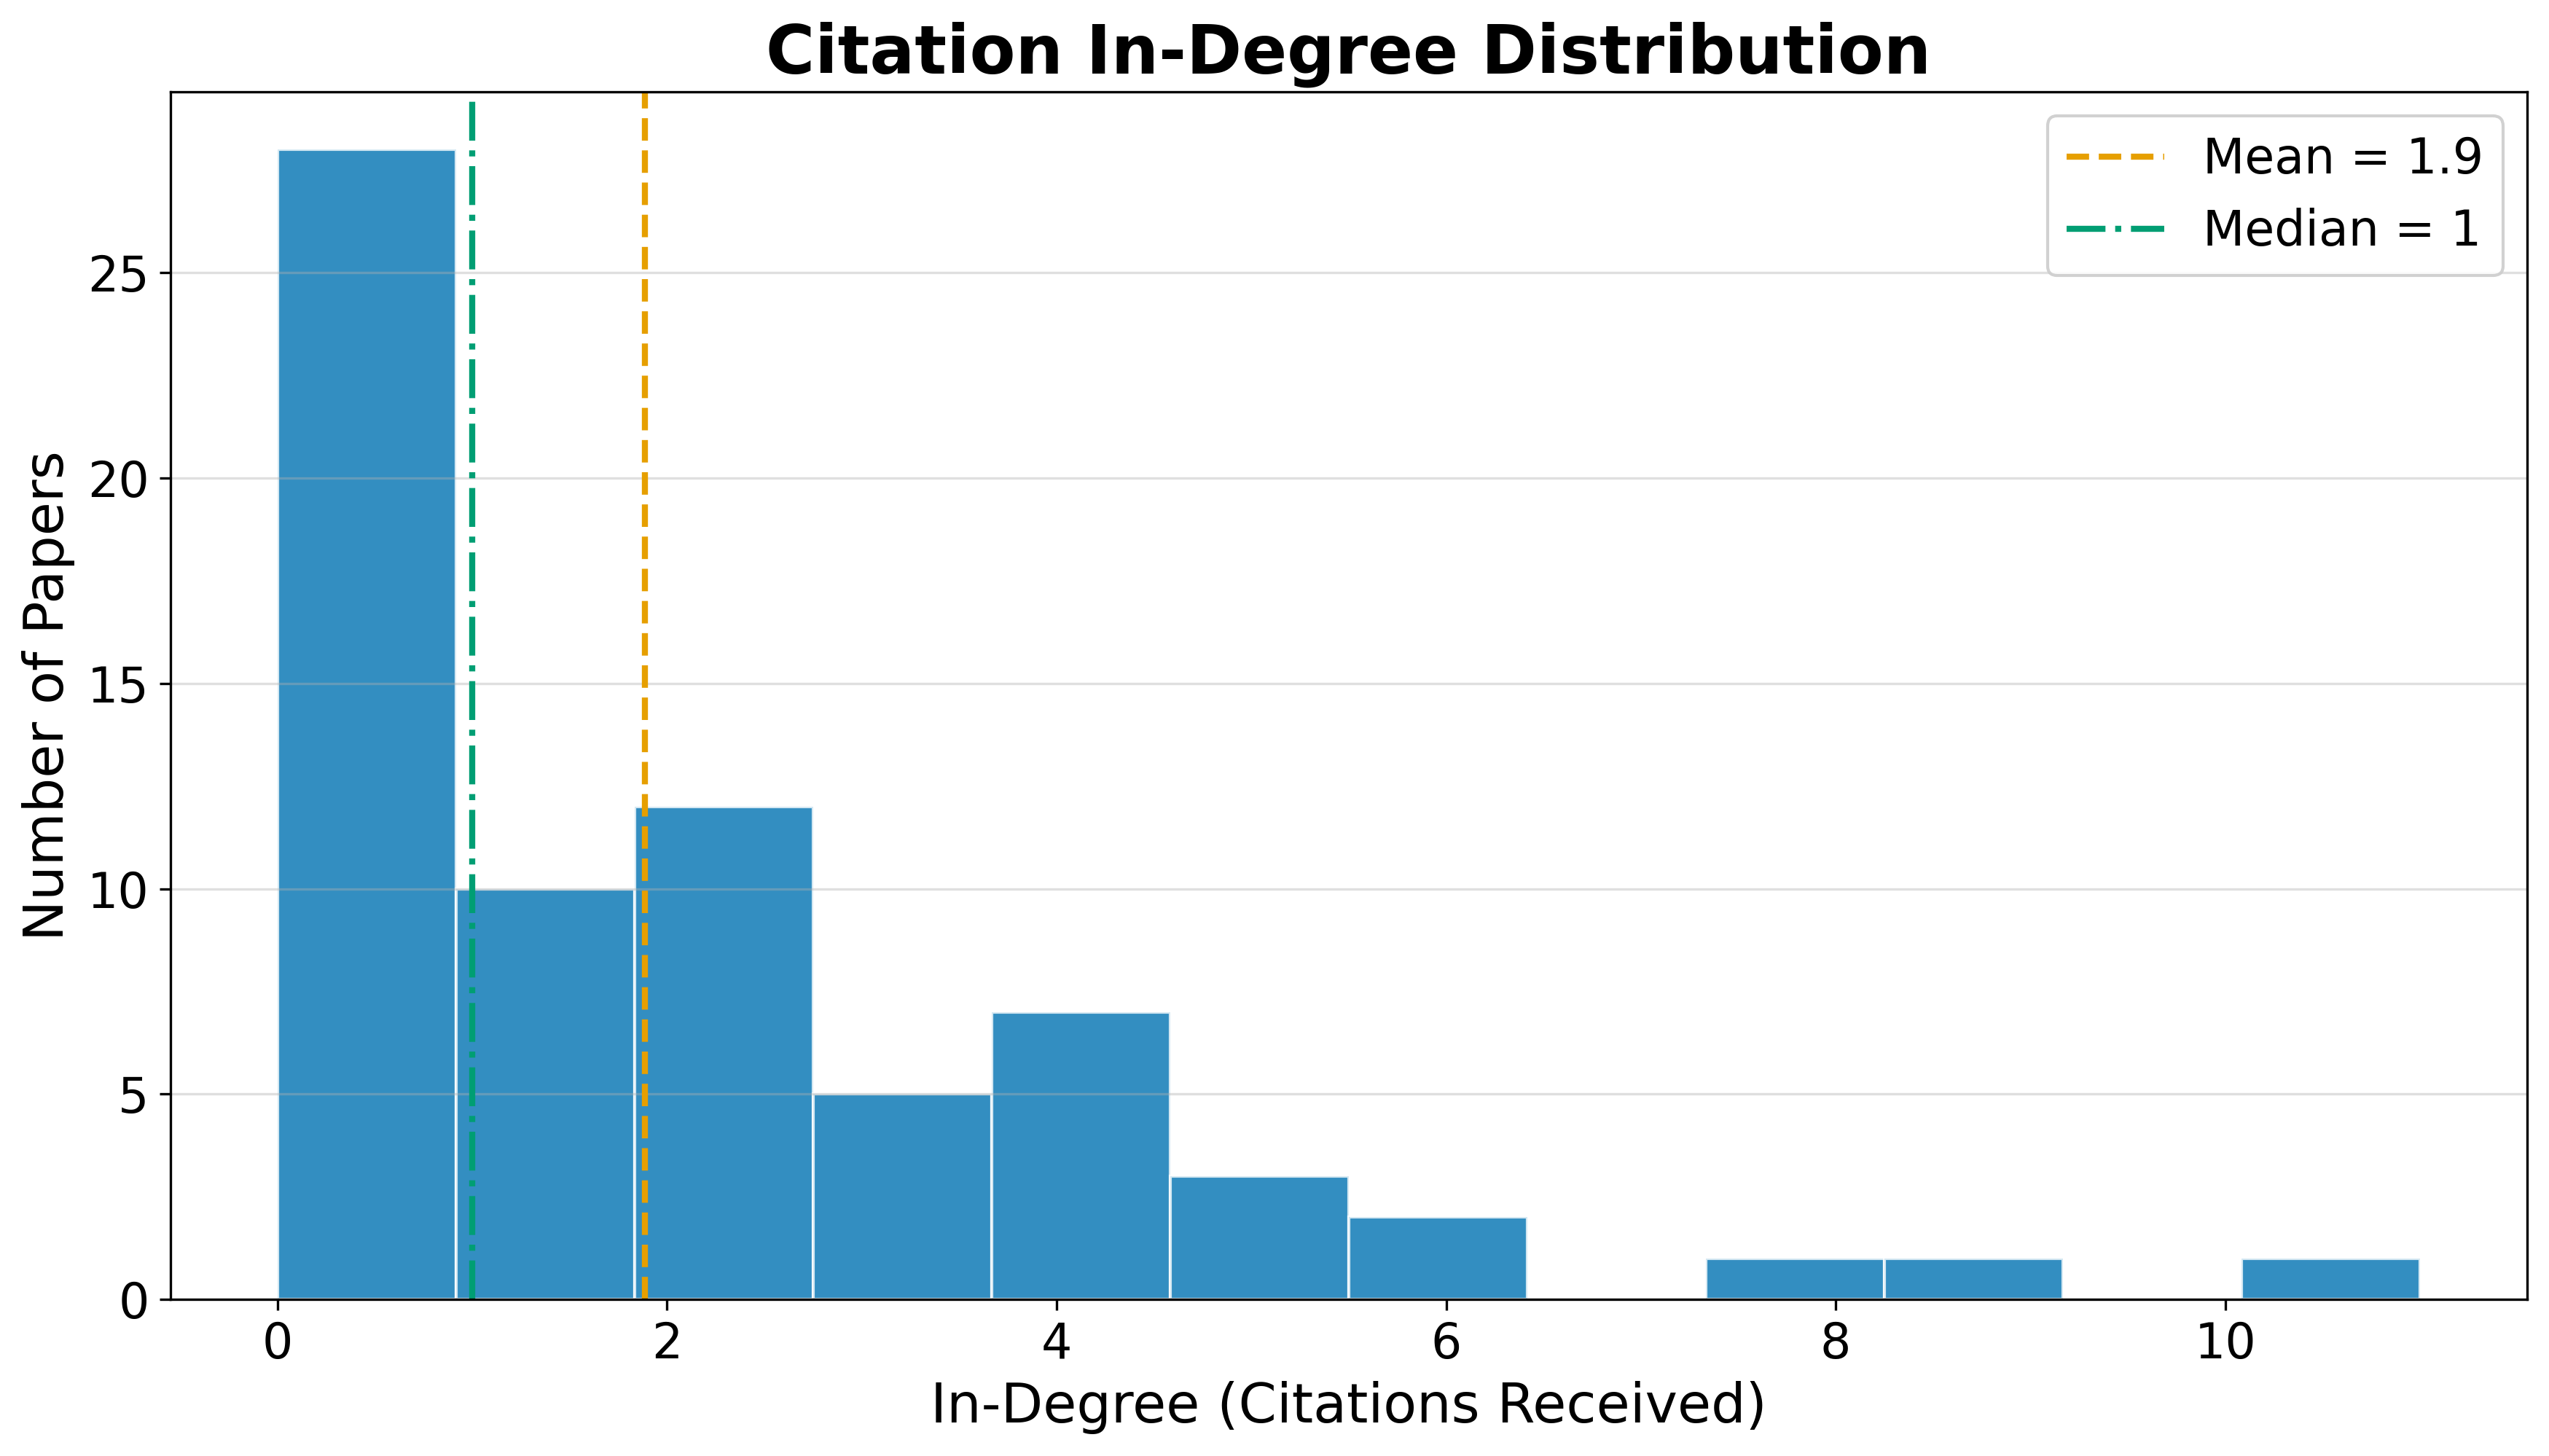
\includegraphics{../figures/degree_distribution.png}
\caption{Degree distribution for the \{\{SEARCH\_TERM\_TITLE\}\}
citation network. The histogram shows the frequency of each in-degree
value on a log-linear scale, revealing the heavy-tailed structure
characteristic of citation networks.}\label{fig:degree_distribution}
\end{figure}

The heavy-tailed degree distribution is characteristic of citation
networks: a small number of highly-cited papers anchor the structure,
while the long tail of low-degree nodes represents newer or peripheral
works. The low graph density (\{\{CITATION\_DENSITY\_PCT\}\}\%) reflects
the sparsity of intra-corpus citation links. Many papers may cite works
outside the retrieved slice, especially under a capped retrieval design.

\subsection{Advanced Network Metrics}\label{advanced-network-metrics}

Beyond PageRank and HITS, the network analysis computes betweenness
centrality (which papers bridge different communities), closeness
centrality (which papers are near all others), degree assortativity (do
highly-cited papers cite other highly-cited papers?), and average
clustering coefficient (how tightly knit are local neighborhoods).

The degree assortativity coefficient is \{\{DEGREE\_ASSORTATIVITY\}\},
and the average clustering coefficient is \{\{AVG\_CLUSTERING\}\}. A
negative assortativity indicates that highly-cited papers tend to cite
less-cited papers (dissortative mixing), which is typical of citation
networks where review papers (high in-degree) cite many primary studies
(low in-degree).

\textbf{Table 7. Top 5 papers by betweenness centrality.}

\{\{TOP\_BETWEENNESS\_TABLE\}\}

Papers with high betweenness centrality occupy shortest paths between
communities in the retained graph. Removing one may alter connectivity,
but that graph operation does not by itself establish that the paper is
a review or methodological bridge in the scientific field. Source-type
and content review are required for that interpretation.

\newpage

\section{Results: Reproducibility
Assessment}\label{results-reproducibility-assessment}

An optional, \textbf{LLM-gated} stage decomposes each paper's described
pipeline into a workflow graph of source, method, experiment, and sink
steps, rates how reproducible each step is from the paper's own text,
and combines a content score with a structural graph-coverage score into
one composite reproducibility score per paper (geometric mean, so a
paper cannot buy a high score by being strong on one axis alone). Across
\{\{REPRODUCIBILITY\_N\_PAPERS\_SCORED\}\} scored papers the mean
composite score is \{\{REPRODUCIBILITY\_MEAN\_SCORE\}\}, with
\{\{REPRODUCIBILITY\_LOW\_SCORE\_COUNT\}\} papers falling below the
configured low-score threshold.

\subsection{Low-Scoring Papers}\label{low-scoring-papers}

Table 8 lists the papers with the lowest composite reproducibility
scores, alongside their content and structural component scores.

\textbf{Table 8. Low-scoring papers by composite reproducibility score.}

\{\{REPRODUCIBILITY\_TABLE\}\}

\subsection{Gating and Defaults}\label{gating-and-defaults-1}

This stage is optional and gated by full-text availability. With no
fulltext available and no language model configured, the stage is
skipped and the reproducibility aggregates read \emph{pending} --- the
same graceful-degradation convention used by the knowledge-graph
assertion-extraction stage (see
\href{02d_methods_knowledge_graph.md}{\breaktt{02d\_methods\_knowledge\_graph.md}}).
When fulltext is available and a language model is explicitly
configured, the mean score, low-score count, and per-paper table are
populated from extracted workflow graphs. The default fixture run does
not imply that this optional model-backed assessment has occurred.

\subsection{Interpretation}\label{interpretation}

A low composite score can reflect either weak content (the paper's own
text does not describe its sources, methods, experiments, or outputs in
enough detail to rate highly) or weak structure (the described steps do
not chain into a coherent source-to-sink pipeline, or reference steps
that were never themselves described). The two axes are reported
separately in Table 8 precisely so a low composite score can be
diagnosed rather than treated as a single undifferentiated verdict.

\newpage

\section{Multi-Phase Results and Cross-Phase
Analysis}\label{multi-phase-results-and-cross-phase-analysis}

\subsection{Phase-Specific Findings}\label{phase-specific-findings}

\subsubsection{Foundation Phase (Phase
1)}\label{foundation-phase-phase-1}

The configured foundation phase retained \{\{PHASE\_1\_PAPERS\}\}
records after its search, filtering, and de-duplication rules. Its
taxonomy includes transit spectroscopy, emission spectroscopy,
phase-curve analysis, and direct imaging. These labels describe the
configured retrieval design; the synthetic fixture cannot establish how
widely those approaches occur in the published literature.

\subsubsection{JWST Phase (Phase 2)}\label{jwst-phase-phase-2}

Phase 2 retained \{\{PHASE\_2\_PAPERS\}\} records under the
JWST-oriented queries and the configured year filter (\texorpdfstring{\textgreater{}=}{>=}2020). The
boundary is intended to include pre-launch calibration work and
post-launch observations. It is a design choice, not evidence that the
phase is exhaustive or that any instrument caused a change in the field.

\subsubsection{Molecular Detection Phase (Phase
3)}\label{molecular-detection-phase-phase-3}

Phase 3 retained \{\{PHASE\_3\_PAPERS\}\} records under five configured
molecule-oriented query groups: H\texorpdfstring{\textsubscript{2}}{2}O, CO\texorpdfstring{\textsubscript{2}}{2}, CH\texorpdfstring{\textsubscript{4}}{4}, H\texorpdfstring{\textsubscript{2}}{2}S, and Na/K. The query
groups operationalize the review question; they do not assert that these
are the most commonly detected species or that the fixture establishes a
scientific trend.

\subsection{Knowledge Graph Results}\label{knowledge-graph-results}

The optional knowledge-graph stage reports
\textbf{\{\{TOTAL\_ASSERTIONS\}\}} assertions from the eligible sample.
The configuration-derived hypothesis table is the authoritative mapping
from review question to score:

\{\{HYPOTHESIS\_TABLE\}\}

The configured scores are descriptive evidence summaries, not calibrated
probabilities, causal effects, or conclusions about instrument
performance. The table should be read together with the claim ledger and
source-tier metadata. A fixture run cannot establish whether models and
observations agree in the broader literature.

\subsection{Citation Network Analysis}\label{citation-network-analysis}

The combined corpus contains \textbf{\{\{CITATION\_EDGES\}\}} citation
relationships across \textbf{\{\{CITATION\_NODES\}\}} papers, with a
network density of \{\{CITATION\_DENSITY\_PCT\}\}\%. This is a
descriptive statistic for the retained corpus; it does not establish a
field-wide citation structure or community claim.

\subsection{Reproducibility
Assessment}\label{reproducibility-assessment}

Reproducibility assessment of the sampled papers revealed a mean
composite reproducibility score of \{\{REPRO\_MEAN\_SCORE\}\}, with
\{\{REPRO\_PAPERS\_SCORED\}\} papers successfully scored. This analysis
examines the computational workflow transparency of each paper,
evaluating source data availability, method documentation, experimental
reproducibility, and output accessibility.

\newpage

\section{Discussion}\label{discussion}

\subsection{Interpretation boundary}\label{interpretation-boundary}

This pipeline describes the shape of a retrieved literature slice: its
phase coverage, metadata completeness, topic structure, citation links,
and declared evidence. It does not adjudicate scientific truth.
Hypothesis scores, when available, summarize recorded assertions and
should be read as evidence-landscape signals rather than calibrated
probabilities.

\subsection{Retrieval and phase bias}\label{retrieval-and-phase-bias}

Engine availability, query wording, rate limits, temporal boundaries,
identifier quality, and full-text access all shape the retained corpus.
The retrieval report is the authoritative account of source outcomes;
counts must never be reverse-engineered from the merged corpus. Phase
overlap and cross-phase citation rates are descriptive checks, not proof
that phases are independent or exhaustive.

\subsection{Fixture and live modes}\label{fixture-and-live-modes}

The offline path uses reserved synthetic identifiers and generated
records. Fixture outputs validate the machinery and its contracts only.
A live review must replace the fixture, retain source-level provenance,
refresh the claim ledger, and obtain domain review before reporting
substantive findings. The manuscript therefore uses explicit pending and
fixture-derived states rather than silently promoting demonstration
values.

\subsection{Limitations and
extensions}\label{limitations-and-extensions}

\begin{itemize}
\tightlist
\item
  Keyword taxonomies can misclassify ambiguous records; changes belong
  in configuration and should be accompanied by a regenerated
  classification report.
\item
  TF-IDF/SVD embeddings are lexical and deterministic; transformer-based
  alternatives require an explicit dependency and evaluation decision.
\item
  LLM extraction is optional, model-sensitive, and not a substitute for
  source review.
\item
  Full-text availability is a coverage measure, not a quality measure.
\item
  Reproducibility claims require a clean double run and normalized
  artifact comparison.
\end{itemize}

These limitations are represented as method-stage and review-required
findings so a publication decision can distinguish deterministic
failures from editorial judgment.

\newpage

\section{Conclusion}\label{conclusion}

This exemplar turns a phase-aware literature-review design into an
auditable, reproducible pipeline. It separates retrieval,
de-duplication, full-text assessment, extraction, bibliometrics,
knowledge-graph construction, visualization, reproducibility assessment,
and export into independently checkable stages.

The central result is architectural: configuration and recorded
artifacts determine the manuscript, while the claim ledger records what
is configured, synthetic, or source-backed. A deterministic fixture run
can prove that the pipeline and validators work; it cannot establish
conclusions about \{\{SEARCH\_TERM\_TITLE\}\}. Live conclusions require
refreshed retrieval evidence, provenance, domain review, and a clean
release audit.

\subsection{Reproducibility}\label{reproducibility}

The rendered manuscript is generated from \breaktt{output/data/*.json},
figures, manifests, registries, and validation reports. A second clean
run should match under the repository's canonical normalized-diff rules.
Any unexplained difference is a release finding. No generated output
should be edited by hand.

\newpage

\section{Appendix A: Tooling and
Reproduction}\label{appendix-a-tooling-and-reproduction}

The pipeline is a two-layer system: generic infrastructure (rendering,
validation, logging) shared across the template monorepo, and
project-local \texttt{src/} modules that implement the meta-analysis.
All numbered \texttt{scripts/} are thin orchestrators that wire I/O,
configuration loading, and logging --- no computational logic resides in
scripts.

\subsection{Reproduce the Offline Default
Run}\label{reproduce-the-offline-default-run}

No network, no language model required:

\begin{Shaded}
\begin{Highlighting}[]
\ExtensionTok{uv}\NormalTok{ run python scripts/generate\_fixture\_corpus.py }\AttributeTok{{-}{-}out}\NormalTok{ output/data/corpus.jsonl}
\ExtensionTok{uv}\NormalTok{ run python scripts/02\_meta\_analysis\_pipeline.py}
\ExtensionTok{uv}\NormalTok{ run python scripts/03\_build\_knowledge\_graph.py }\AttributeTok{{-}{-}max{-}papers}\NormalTok{ 0}
\ExtensionTok{uv}\NormalTok{ run python scripts/04\_generate\_figures.py }\AttributeTok{{-}{-}dpi}\NormalTok{ 300}
\ExtensionTok{uv}\NormalTok{ run python scripts/05\_inject\_variables.py}
\end{Highlighting}
\end{Shaded}

\subsection{Reproduce the Live Run}\label{reproduce-the-live-run}

This manuscript was generated from a live retrieval run. To reproduce:

\begin{Shaded}
\begin{Highlighting}[]
\CommentTok{\# Live search (all 9 engines, max 1000 per engine)}
\ExtensionTok{uv}\NormalTok{ run python scripts/01\_literature\_search.py }\AttributeTok{{-}{-}query}\NormalTok{ modafinil }\AttributeTok{{-}{-}max{-}results}\NormalTok{ 1000 }\AttributeTok{{-}{-}no{-}resume}

\CommentTok{\# Analysis pipeline}
\ExtensionTok{uv}\NormalTok{ run python scripts/02\_meta\_analysis\_pipeline.py}
\ExtensionTok{uv}\NormalTok{ run python scripts/03\_build\_knowledge\_graph.py }\AttributeTok{{-}{-}max{-}papers}\NormalTok{ 0}
\ExtensionTok{uv}\NormalTok{ run python scripts/04\_generate\_figures.py }\AttributeTok{{-}{-}dpi}\NormalTok{ 300}
\ExtensionTok{uv}\NormalTok{ run python scripts/05\_inject\_variables.py}
\ExtensionTok{uv}\NormalTok{ run python scripts/06\_fulltext\_assessment.py}
\ExtensionTok{uv}\NormalTok{ run python scripts/07\_literature\_evaluation.py}
\ExtensionTok{uv}\NormalTok{ run python scripts/09\_export\_bibliography.py}
\end{Highlighting}
\end{Shaded}

\subsection{Re-target to Another
Topic}\label{re-target-to-another-topic}

Edit \breaktt{manuscript/config.yaml} ---
\breaktt{project\_config.search.term}, \texttt{query},
\breaktt{relevance\_keywords}, \breaktt{subfield\_keywords}, and
\breaktt{hypothesis\_definitions} --- then regenerate the seed corpus and
re-run. No code changes are required; the manuscript re-targets through
token injection.

\subsection{Live Retrieval}\label{live-retrieval}

Enable engines under \breaktt{project\_config.search.engines}, supply any
optional credentials (Unpaywall email, Semantic Scholar key), and run
\breaktt{scripts/01\_literature\_search.py}; absent engines degrade to
skipped sources. The CLI supports per-engine skip flags:
\texttt{-\/-skip-arxiv}, \texttt{-\/-skip-s2},
\breaktt{-\/-skip-openalex}, \breaktt{-\/-skip-crossref},
\texttt{-\/-skip-pubmed}, \breaktt{-\/-skip-sovietrxiv},
\breaktt{-\/-skip-chinarxiv}, \breaktt{-\/-skip-europepmc},
\breaktt{-\/-skip-biorxiv}.

\subsection{Deep Research (Offline Fixture
Replay)}\label{deep-research-offline-fixture-replay}

This exemplar also demonstrates the shared
\breaktt{infrastructure.search.deep\_research} capability ---
provider-neutral dispatch to OpenAI and Gemini deep-research agents.
Because deep research is a \textbf{paid, non-deterministic} service, the
template never calls it live in CI. Instead,
\breaktt{src/deep\_research/dispatch.py} wires the real infrastructure
request/result models (\breaktt{DeepResearchConfig},
\breaktt{DeepResearchRequest}, \breaktt{DeepResearchResult},
\breaktt{DeepResearchClient}) and ships a deterministic, offline path:
\breaktt{scripts/08\_deep\_research\_dispatch.py} builds the genuine
provider-neutral request and then \emph{replays} a recorded report
fixture (\breaktt{src/deep\_research/fixtures/recorded\_report.json}),
normalizing it through the real \breaktt{DeepResearchResult} model.
Replay fails closed if the fixture is missing --- it never fabricates a
passing run --- mirroring the fixture-replay idiom of
\texttt{template\_sia}. The same source module constructs the exact
\breaktt{DeepResearchRequest} a live \texttt{submit} would dispatch, so a
fork can enable real providers behind an explicit live-only command:

\begin{Shaded}
\begin{Highlighting}[]
\CommentTok{\# Offline (default): replays the recorded report, no key required}
\ExtensionTok{uv}\NormalTok{ run python scripts/08\_deep\_research\_dispatch.py}
\end{Highlighting}
\end{Shaded}

\subsection{Test Suite}\label{test-suite}

Every stage is covered by a no-mocks test suite (real computation and
\breaktt{pytest-httpserver} for network adapters) gated at \(\geq 90\%\)
statement coverage on \texttt{src/}. The suite covers:

\begin{itemize}
\tightlist
\item
  Record models and serialization (deduplication, canonical ID
  hierarchy)
\item
  All 9 engine clients (arXiv, Semantic Scholar, OpenAlex, Crossref,
  PubMed, SovietRxiv, ChinaRxiv, Europe PMC, bioRxiv/medRxiv) with
  pytest-httpserver integration tests
\item
  Search runner (multi-engine dispatch, relevance filtering,
  resume/clear, YAML config)
\item
  Bibliometric analysis (subfield classification, temporal metrics,
  TF-IDF, NMF, citation network)
\item
  Knowledge graph (schema, nanopublications, hypothesis scoring, LLM
  extraction)
\item
  Visualization (headless figure generation, style config)
\item
  Manuscript variable computation and injection
\end{itemize}

\newpage

\section{Appendix B: Technical Notes}\label{appendix-b-technical-notes}

\subsection{Determinism}\label{determinism}

All stochastic steps use fixed seeds (seed = 42 for NMF, SVD, and graph
layouts). The fixture corpus, TF-IDF/SVD embeddings, and topic
factorization are byte-stable across runs. Graph centrality scores are
rounded to a fixed precision and ranked with a node-id tiebreaker so
that floating-point non-associativity in iterative solvers cannot
perturb the reported rankings. Record identity uses a content digest
(SHA-1, \breaktt{usedforsecurity=False}) rather than a salted hash, so
de-duplication and corpus byte-stability hold across processes.

\subsection{Data Model}\label{data-model}

Each record is a \texttt{Paper} dataclass with: title, abstract, authors
(list of \texttt{Author}), year, DOI, arXiv ID, Semantic Scholar ID,
OpenAlex ID, venue, citation count, references (list of canonical IDs),
publication date, PDF URL, open-access flag, and full-text source. The
canonical identifier hierarchy governs de-duplication and citation
resolution:

\[
\text{canonical\_id} = \begin{cases}
\texttt{doi:} + \text{normalize}(\text{DOI}) & \text{if DOI present} \\
\texttt{arxiv:} + \text{arXiv\_id} & \text{if arXiv ID present} \\
\texttt{s2:} + \text{S2\_id} & \text{if S2 ID present} \\
\texttt{openalex:} + \text{OpenAlex\_id} & \text{if OpenAlex ID present} \\
\texttt{title:} + \text{SHA1}(\text{title})[:16] & \text{otherwise}
\end{cases}
\]

DOI normalization lower-cases the DOI and strips any
\breaktt{https://doi.org/} or \texttt{dx.doi.org/} prefix, so the same
paper returned by two engines under different case or format variants
merges to a single canonical ID.

\subsection{NMF Mathematics}\label{nmf-mathematics}

Non-negative matrix factorization decomposes the TF-IDF document-term
matrix \(\mathbf{V} \in \mathbb{R}^{m \times n}\) (where \(m\) is the
number of documents and \(n\) is the vocabulary size) into
\(\mathbf{W} \in \mathbb{R}^{m \times k}\) and
\(\mathbf{H} \in \mathbb{R}^{k \times n}\), where \(k\) is the number of
topics (here \{\{NUM\_TOPICS\}\}). The factorization minimizes:

\[
\min_{\mathbf{W}, \mathbf{H} \geq 0} \|\mathbf{V} - \mathbf{W} \mathbf{H}\|_F^2
\]

using multiplicative update rules \citep{lee1999learning} with a fixed
random seed for reproducibility. The topic-term matrix \(\mathbf{H}\)
gives the top terms per topic; the document-topic matrix \(\mathbf{W}\)
gives each document's topic loadings.

\subsection{Growth Rate Estimation}\label{growth-rate-estimation}

The compound annual growth rate is:

\[
\text{CAGR} = \left(\frac{N_{\text{end}}}{N_{\text{start}}}\right)^{1/(T_{\text{end}} - T_{\text{start}})} - 1
\]

where \(N_{\text{start}}\) and \(N_{\text{end}}\) are the publication
counts in the first and last years of the corpus, respectively. The
doubling time is \(t_d = \ln(2) / \ln(1 + \text{CAGR})\). For this run:
CAGR = \{\{CAGR\_PCT\}\}\%, doubling time = \{\{DOUBLING\_TIME\}\}
years.

\subsection{Configuration Surface}\label{configuration-surface-1}

A single \breaktt{manuscript/config.yaml} controls the search term,
per-engine query and keyword sets, engine enable toggles, subfield
taxonomy, hypotheses, full-text and embedding options, and paper
metadata. This run drew on \{\{N\_ENGINES\}\} engines, a
\{\{N\_SUBFIELDS\}\}-bucket taxonomy, and \{\{N\_HYPOTHESES\}\}
hypotheses.

\subsection{Artifacts}\label{artifacts}

Intermediate and final outputs live under \texttt{output/} and are
disposable and regenerable:

\begin{longtable}[]{@{}
  >{\raggedright\arraybackslash}p{(\columnwidth - 4\tabcolsep) * \real{0.3333}}
  >{\raggedright\arraybackslash}p{(\columnwidth - 4\tabcolsep) * \real{0.3333}}
  >{\raggedright\arraybackslash}p{(\columnwidth - 4\tabcolsep) * \real{0.3333}}@{}}
\toprule\noalign{}
\begin{minipage}[b]{\linewidth}\raggedright
File
\end{minipage} & \begin{minipage}[b]{\linewidth}\raggedright
Stage
\end{minipage} & \begin{minipage}[b]{\linewidth}\raggedright
Description
\end{minipage} \\
\midrule\noalign{}
\endhead
\bottomrule\noalign{}
\endlastfoot
\texttt{corpus.jsonl} & 01 & De-duplicated corpus (\{\{CORPUS\_SIZE\}\}
records) \\
\breaktt{temporal\_analysis.json} & 02 & Year counts, CAGR, doubling
time, peak year \\
\breaktt{subfield\_classification.json} & 02 & Per-bucket paper counts \\
\breaktt{subfield\_timeline.json} & 02 & Per-subfield annual breakdown \\
\texttt{tfidf\_data.json} & 02 & TF-IDF matrix, feature names, doc
tokens \\
\texttt{topics.json} & 02 & NMF topic-term distributions \\
\breaktt{citation\_network.json} & 02 & Network metrics, PageRank, HITS,
communities \\
\breaktt{citation\_graph.gml} & 02 & GraphML citation graph \\
\breaktt{nanopublications.jsonl} & 03 & LLM-extracted assertions (0 in
this run) \\
\breaktt{hypothesis\_scores.json} & 03 & Per-hypothesis evidence
scores \\
\breaktt{fulltext\_assessment.json} & 06 & Abstract/OA/PDF coverage
report \\
\end{longtable}

\newpage

\section{Appendix C: Accessibility and
Provenance}\label{appendix-c-accessibility-and-provenance}

\subsection{Figure Accessibility}\label{figure-accessibility}

All \{\{NUM\_FIGURES\}\} figures are rendered with a colourblind-safe
palette (Wong 2011, 8 colours) and high-contrast labels at publication
DPI (300). Each figure carries a descriptive caption so the visual
claims are recoverable from text alone. The palette avoids red-green
colour pairs that are indistinguishable for deuteranopia and protanopia;
when more than 8 categories are needed, continuous colormaps
(\texttt{viridis}, \texttt{plasma}) are used instead of extending the
discrete palette. Font sizes are enforced at \(\geq 16\)pt via a
centralized style module, ensuring readability at both screen and print
sizes.

\subsection{Provenance Chain}\label{provenance-chain}

Every reported number is injected from a committed artifact rather than
typed by hand; an unresolved placeholder is a hard error, so the
rendered manuscript can contain no orphaned or stale figures. The
configuration hash and artifact inventory bind the prose to the exact
pipeline run that produced it. The provenance chain is:

\begin{enumerate}
\def\labelenumi{\arabic{enumi}.}
\tightlist
\item
  \breaktt{manuscript/config.yaml} defines the search term, engines,
  taxonomy, and hypotheses
\item
  \breaktt{scripts/01\_multi\_phase\_search.py} retrieves or fixtures
  records \texorpdfstring{\ensuremath{\to}}{->} \texttt{corpus.jsonl}
\item
  \breaktt{scripts/02\_meta\_analysis\_pipeline.py} analyses the corpus \texorpdfstring{\ensuremath{\to}}{->}
  \texttt{*.json} data files
\item
  \breaktt{scripts/04\_generate\_figures.py} renders figures \texorpdfstring{\ensuremath{\to}}{->}
  \texttt{*.png} + \breaktt{figure\_registry.json}
\item
  \breaktt{scripts/05\_inject\_variables.py} computes variables from data
  files \texorpdfstring{\ensuremath{\to}}{->} manuscript text
\end{enumerate}

Each figure in \breaktt{figure\_registry.json} records its source data
file, generation parameters, and SHA-256 hash, binding the visual output
to the exact pipeline run. Re-running the pipeline with the same
configuration and seed produces identical data outputs.

\subsection{FAIR Data Principles}\label{fair-data-principles}

The pipeline supports FAIR (Findable, Accessible, Interoperable,
Reusable) data principles:

\begin{itemize}
\tightlist
\item
  \textbf{Findable}: Each record carries persistent identifiers (DOI,
  arXiv ID, OpenAlex ID) that make it findable across databases.
\item
  \textbf{Accessible}: The corpus is stored as plain JSONL, readable by
  any JSON parser; figures are standard PNG files.
\item
  \textbf{Interoperable}: The data model uses standard bibliographic
  fields (title, abstract, authors, DOI, year, venue); nanopublications
  are serialized as RDF/TriG.
\item
  \textbf{Reusable}: The entire pipeline is regenerable from
  \breaktt{manuscript/config.yaml}; re-running with the same
  configuration reproduces identical outputs.
\end{itemize}

\subsection{Honesty}\label{honesty}

The default corpus is synthetic and labelled as such; the manuscript
does not present fixture-derived numbers as empirical findings about
\{\{SEARCH\_TERM\}\}. Live findings require a real retrieval run with
regenerated artifacts and source-level provenance.

\newpage

\section{Glossary}\label{glossary}

\begin{longtable}[]{@{}
  >{\raggedright\arraybackslash}p{(\columnwidth - 2\tabcolsep) * \real{0.5000}}
  >{\raggedright\arraybackslash}p{(\columnwidth - 2\tabcolsep) * \real{0.5000}}@{}}
\toprule\noalign{}
\begin{minipage}[b]{\linewidth}\raggedright
Term
\end{minipage} & \begin{minipage}[b]{\linewidth}\raggedright
Meaning
\end{minipage} \\
\midrule\noalign{}
\endhead
\bottomrule\noalign{}
\endlastfoot
\textbf{Record / Paper} & A single bibliographic entry with metadata and
identifiers. \\
\textbf{Canonical identifier} & The highest-priority available ID (DOI
\(>\) arXiv \(>\) Semantic Scholar \(>\) OpenAlex \(>\) title digest)
used for de-duplication and citation resolution. \\
\textbf{Engine} & An independent literature source adapter
(\{\{ENGINE\_LIST\}\}) with a uniform search interface and graceful
skip-on-failure. \\
\textbf{Subfield} & One of the \{\{N\_SUBFIELDS\}\} configurable
keyword-defined buckets (\{\{SUBFIELD\_LIST\}\}) into which records are
classified. \\
\textbf{Topic} & A latent theme from non-negative matrix factorization
over the TF-IDF representation. \\
\textbf{Embedding} & A deterministic offline vector (TF-IDF
\(\rightarrow\) truncated SVD) for a title, abstract, or full text. \\
\textbf{Hypothesis} & One of the \{\{N\_HYPOTHESES\}\} configured claims
about the topic, optionally scored by the knowledge-graph stage. \\
\textbf{Assertion} & A directional (supports / contradicts / neutral)
statement extracted from a record against a hypothesis, with a
confidence score. \\
\textbf{Nanopublication} & An RDF-serialized assertion plus its
provenance. \\
\textbf{CAGR} & Compound annual growth rate of publication volume
(\{\{CAGR\_PCT\}\}\% for this corpus). \\
\textbf{Living literature review} & A synthesis that can be re-executed
as the field evolves, with every number regenerable. \\
\end{longtable}

\newpage

\section{References}\label{references}

The bibliography is generated automatically during PDF compilation from
\texttt{references.bib}. Every citation key used in the manuscript has a
matching bibliography entry, and the checked-in bibliography contains
only sources required by the manuscript sections. Pandoc's
\texttt{-\/-natbib} flag injects
\texttt{\textbackslash{}usepackage\{natbib\}} and
\texttt{\textbackslash{}bibliographystyle\{plainnat\}}, so neither
directive appears in this section or in \texttt{preamble.md}.

\providecommand{\bibsection}{}
\renewcommand{\bibsection}{}

\bibliography{references}

\end{document}
